\pdfoutput=1
\documentclass[12pt]{article} 
\usepackage{sastyle} 
\usepackage{alphalph}
\graphicspath{ {images/} }

\newcommand\draftnote[1]{{\color{blue} #1}}

\newtheorem{exercise}{Exercise}[section]
\let\Exercisefont\itshape
\def\Exerciseheadfont{\bfseries}

\makeatletter
\newalphalph{\alphmult}[alph]{\@alph}{26}
\makeatother
\renewcommand{\thefootnote}{\alphmult{\value{footnote}}}

\numberwithin{equation}{section}

\def\naive{naïve }
\def\naively{naïvely }

%%%%%%%%%%%%%%% FRONT PAGE %%%%%%%%%%%%%%%%%
\begin{document}
	\vspace*{-.6in} \thispagestyle{empty}
	\begin{flushright}
	\end{flushright}
	\vspace{.2in} {\Large
		\begin{center}
			{\bf Conformal Symmetry in Field Theories\vspace{.1in}}
		\end{center}
	}
	\vspace{.2in}
	\begin{center}
		{\bf 
			Soner Albayrak\footnote{\href{mailto:contact@soneralbayrak.com}{contact@soneralbayrak.com}}
		\\
		\vspace{.2in} 
		{\it  Institute of Physics, University of Amsterdam, Amsterdam, 1098 XH, The Netherlands}}
	\end{center}
	
	\vspace{.2in}

%	\begin{abstract}
		These are the notes of the lectures prepared for the ``Advanced Topics in Theoretical Physics''  summer school at \emph{Feza Gürsey Merkezi}, September 2021. These notes are mostly based on other discussions and I provided the sources  in relevant places. I may update the notes even after the summer school to keep it up-to-date and self-contained; there are also reminders \draftnote{in blue} for me to add further discussion/comments.
		\par This document was last updated on \today.
%	\end{abstract}
	
	\newpage

\tableofcontents
\clearpage
\addcontentsline{toc}{subsection}{Literature Recommendations}%
\section*{Literature Recommendations}
One can find many books, reviews, lecture notes, and articles about \emph{conformal symmetry}, \emph{conformal bootstrap program}, \emph{quantum theory of fields}, \emph{renormalization group}, \emph{critical phenomena}, \emph{AdS/CFT correspondence}, \emph{cosmological bootstrap}, \emph{flat space holography}, \emph{string theory} and many other related concepts to conformal symmetry and its usage in theoretical physics. You can go ahead and search these keywords and see how large a literature there exists for each and every one of these topics.

So finding a source for conformal symmetry or its usage is no problem, it is the other way around: there are simply too many resources and one can feel overwhelmed and find it hard to navigate through those articles to learn the subject. So below, I'll list some resources that I would recommend both to \naive younglings who know nothing about these subjects and to those physics-hardened veterans who have heard of/worked on some of these subjects but haven't really got the chance to look at conformal symmetry directly. Please note that the list is \emph{faaaaar} from being complete and in no means is supposed to include good resources and to exclude bad ones: I simply listed what I know (and would recommend) and it is extremely likely that there are reviews out there that would be far more suited yet are unbeknownst to me.

\begin{enumerate}
	\item The traditional referencing source for conformal symmetry is the so-called \emph{yellow book}, i.e. \emph{Conformal Field Theory} by Francesco, Mathieu, and Sénéchal. It is a rather complete book, i.e. it covers all the basics, however it is published in 1997 and hence does not include recent developments captured by \emph{conformal bootstrap program}. In short, conformal symmetry is a lot easier to solve in two spacetime dimensions and up until the last two decades all the major progress has been in two dimensions, hence naturally most of the book's content is for two dimensional conformal models.
	\item The de facto referencing source for the conformal bootstrap program (which aims to constraint or solve conformal models in higher dimensions, i.e. $d\ge 3$) is the review article \emph{The Conformal Bootstrap: Theory, Numerical Techniques, and Applications} by Poland (who happens to be my PhD advisor\footnote{Thus I may be biased towards his work due to more exposure.}), Rychkov, and Vichi. The article really does not get into details (and not really pedagogical), so it is not the best source to \emph{learn} stuff. However, it is an excellent collection of sources, so one can use it to find other sources for individual topics.
	\item The de facto lecture notes to learn the basics of the conformal symmetry is \emph{TASI Lectures on the Conformal Bootstrap} by Simmons-Duffin (who happens to be my host during my 1-year visit to Caltech\footnote{Thus I may be biased towards his work due to more exposure.}). Around similar times, Qualls shared his lecture notes \emph{Lectures on Conformal Field Theory} as well (which is less focused on bootstrap but more on 2d CFTs).\footnote{There is also the lecture notes \emph{Applied Conformal Field Theory} by Ginsparg. Honestly, I did not fully read the notes as they are rather focused on $2d$ CFTs which are not really my personal focus; however, some may find them quite useful.} A more recent review was given by Osborn, i.e. \emph{Lectures on Conformal Field Theories in more than two dimensions}, however they are somehow more technical and less pedagogical.
	\item Slava Rychkov maintains an active blog where he writes about his papers or his talks among other useful information, see \hyperref{https://sites.google.com/site/slavarychkov}{}{}{https://sites.google.com/site/slavarychkov}. He also wrote lecture notes titled \emph{EPFL Lectures on Conformal Field Theory in D>= 3 Dimensions}, it is a bit older than Simmons-Duffin's lecture notes, but some may prefer the style. He also talked about the \emph{philosophy} of the bootstrap approach as the $27^{\text{th}}$ Ockham Lecture, see \hyperref{https://www.merton.ox.ac.uk/event/27th-ockham-lecture-reductionism-vs-bootstrap-are-things-big-always-made-things-elementary}{}{}{https://www.merton.ox.ac.uk/event/27th-ockham-lecture-reductionism-vs-bootstrap-are-things-big-always-made-things-elementary}.
	
	\item If you would like a \emph{hardcore} resource, then there is the \emph{holy book}.\footnote{See \hyperref{http://doi.org/10.1007/BFb0009678}{}{}{http://doi.org/10.1007/BFb0009678}.} It is written by Dobrev, Mack, Petkova's, and Todorov in 1977 and is still extremely relevant today. The only problem is that it is rather mathematical (and technical), and you may find it hard --- honestly I did not fully read the book myself, I only have used it as a reference to check stuff here and there. 
	\item If you would like a \emph{layman review} of the conformal bootstrap, then I'd suggest the nature article of Poland and Simmons-Duffin, i.e. \hyperref{https://doi.org/10.1038/nphys3761}{}{}{https://doi.org/10.1038/nphys3761}.
	
	\item If you prefer \emph{watching} to \emph{reading}, then there are recordings of excellent lectures in the summer schools of the conformal bootstrap collaboration.\footnote{See \hyperref{http://bootstrapcollaboration.com/activities}{}{}{http://bootstrapcollaboration.com/activities}} You can also view all videos of the collaboration at their Youtube channel:\footnote{See \hyperref{https://www.youtube.com/channel/UCgWLG2q2275RuUJ5eNSCCFA/videos}{}{}{https://www.youtube.com/channel/UCgWLG2q2275RuUJ5eNSCCFA/videos}.} I personally advice 2017 \& 2018 Bootstrap School videos as they were rather introductory and pedagogical!
	
	\item These lectures will be mostly about conformal symmetry in $d\ge 3$ spacetime dimensions, hence $d=2$ conformal symmetry (and related Virasoro symmetry) are not our focus. For those interested in $d=2$ conformal symmetry (and its utility in String theory), I already named a few sources, but there are two books I would like to refer for sentimental reasons:  \emph{String and Symmetries}, edited by Gülen Aktaş, Cihan Saçlıoğlu, and Meral Serdaroğlu; and \emph{Conformal Field Theory: New Non-perturbative Methods In String And Field Theory}, edited by Yavuz Nutku, Cihan Saçlıoğlu, and Teoman Turgut. The former book consists of the proceedings of the Feza Gürsey Memorial Conference 1 (1994); and the latter book consists of lecture notes of  \emph{1998 Summer Research Semester on Conformal Field Theories, M(atrix) Models and Dualities}; both events held at Bogaziçi Üniversitesi-Tübitak Feza Gürsey Institute.
	
	\item Lastly, I can recommend the first two chapters of my thesis as \emph{an earnest attempt at a very pedagogical introduction} to conformal symmetry and the conformal bootstrap program. I tried to give a historical account of the subject, its basics, and recent developments. Even if you don't like it, you may find the references useful as I tried my best to organize and include as many references as possible. You can find it via the publisher's website\footnote{See \hyperref{https://www.proquest.com/docview/2557212384/2C5A80A2ADB447E7PQ}{}{}{https://www.proquest.com/docview/2557212384/2C5A80A2ADB447E7PQ}.} or via arXiv.\footnote{See \hyperref{https://arxiv.org/abs/2107.13601}{}{}{https://arxiv.org/abs/2107.13601}.}
\end{enumerate}


\clearpage
\listoffigures
\addcontentsline{toc}{subsection}{\listfigurename}%
\listoftables
\addcontentsline{toc}{subsection}{\listtablename}%
\clearpage

\newpage

% BODY

\section{Why conformal symmetry?}
\subsection{Invitation: Critical phenomena}
\subsubsection{A brief review of phase diagrams}
Let us start with something we observe in everyday life and have been taught in kindergarten: matter exists in different phases. These phases can be differentiated by macroscopic parameters such as  viscosity and compressibility; as we are all well aware by our everyday experiences, this translates into fluids having three different phases: \emph{solid} (high viscosity \& low compressibility), \emph{liquid} (low viscosity \& low compressibility), and \emph{gaseous} (low viscosity \& high compressibility). By changing the pressure and the temperature, we can change the phase of a fluid; the landscape of all phases of a given substance is shown in \emph{a phase diagram}, e.g. \figref{\ref{fig: phase diagram}}.

\begin{figure}
	\centering 
	$(a)\begin{aligned}
		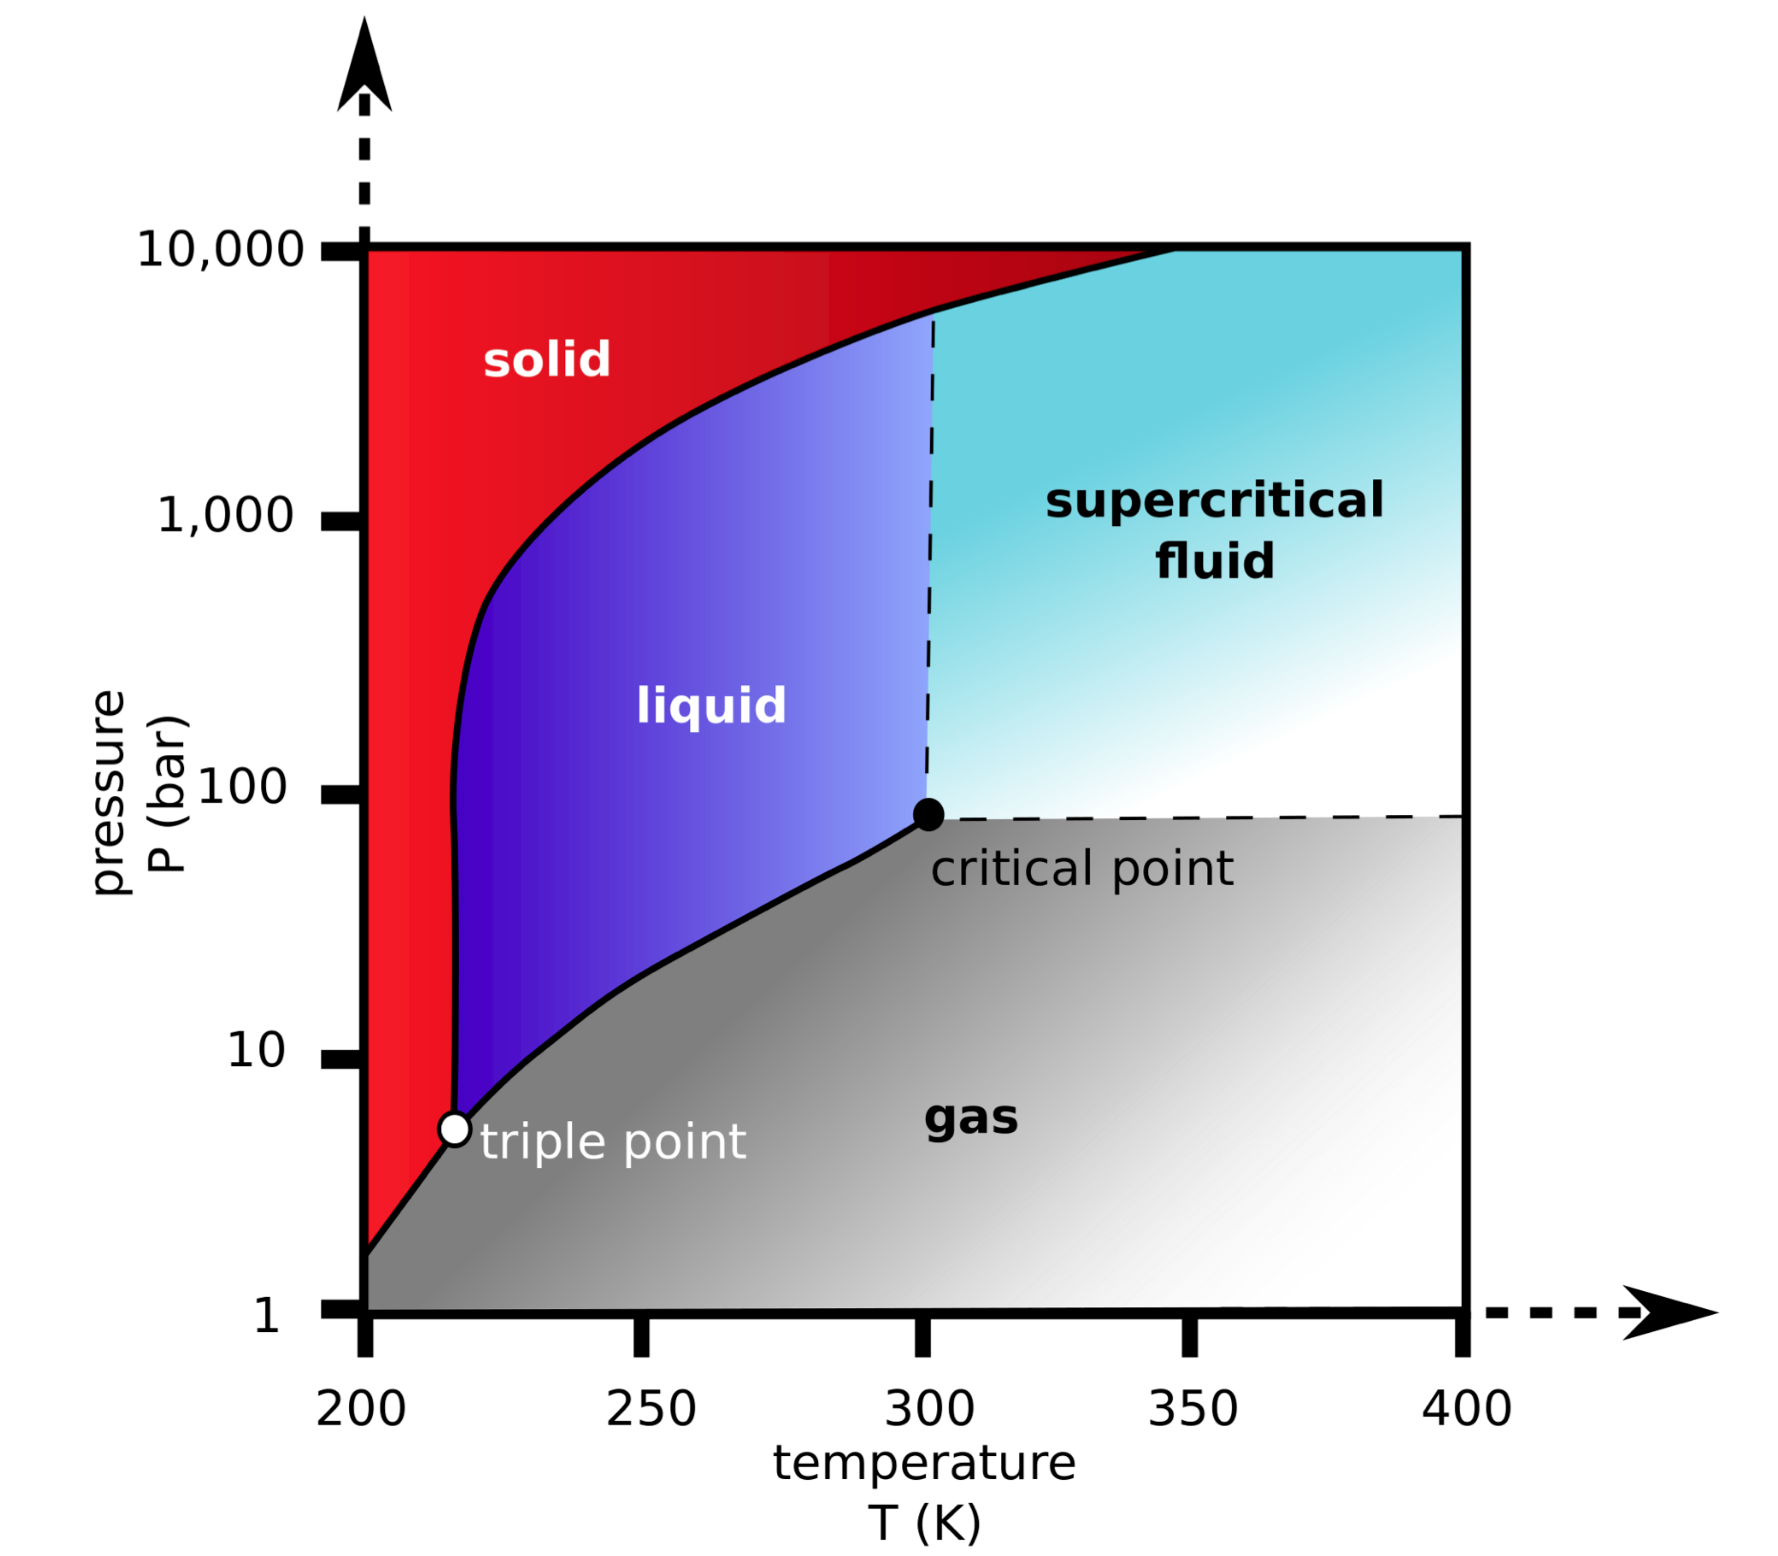
\includegraphics[scale=.22]{phase_diagram.png}
	\end{aligned}\quad 
	(b)\;\;
	\begin{aligned}
		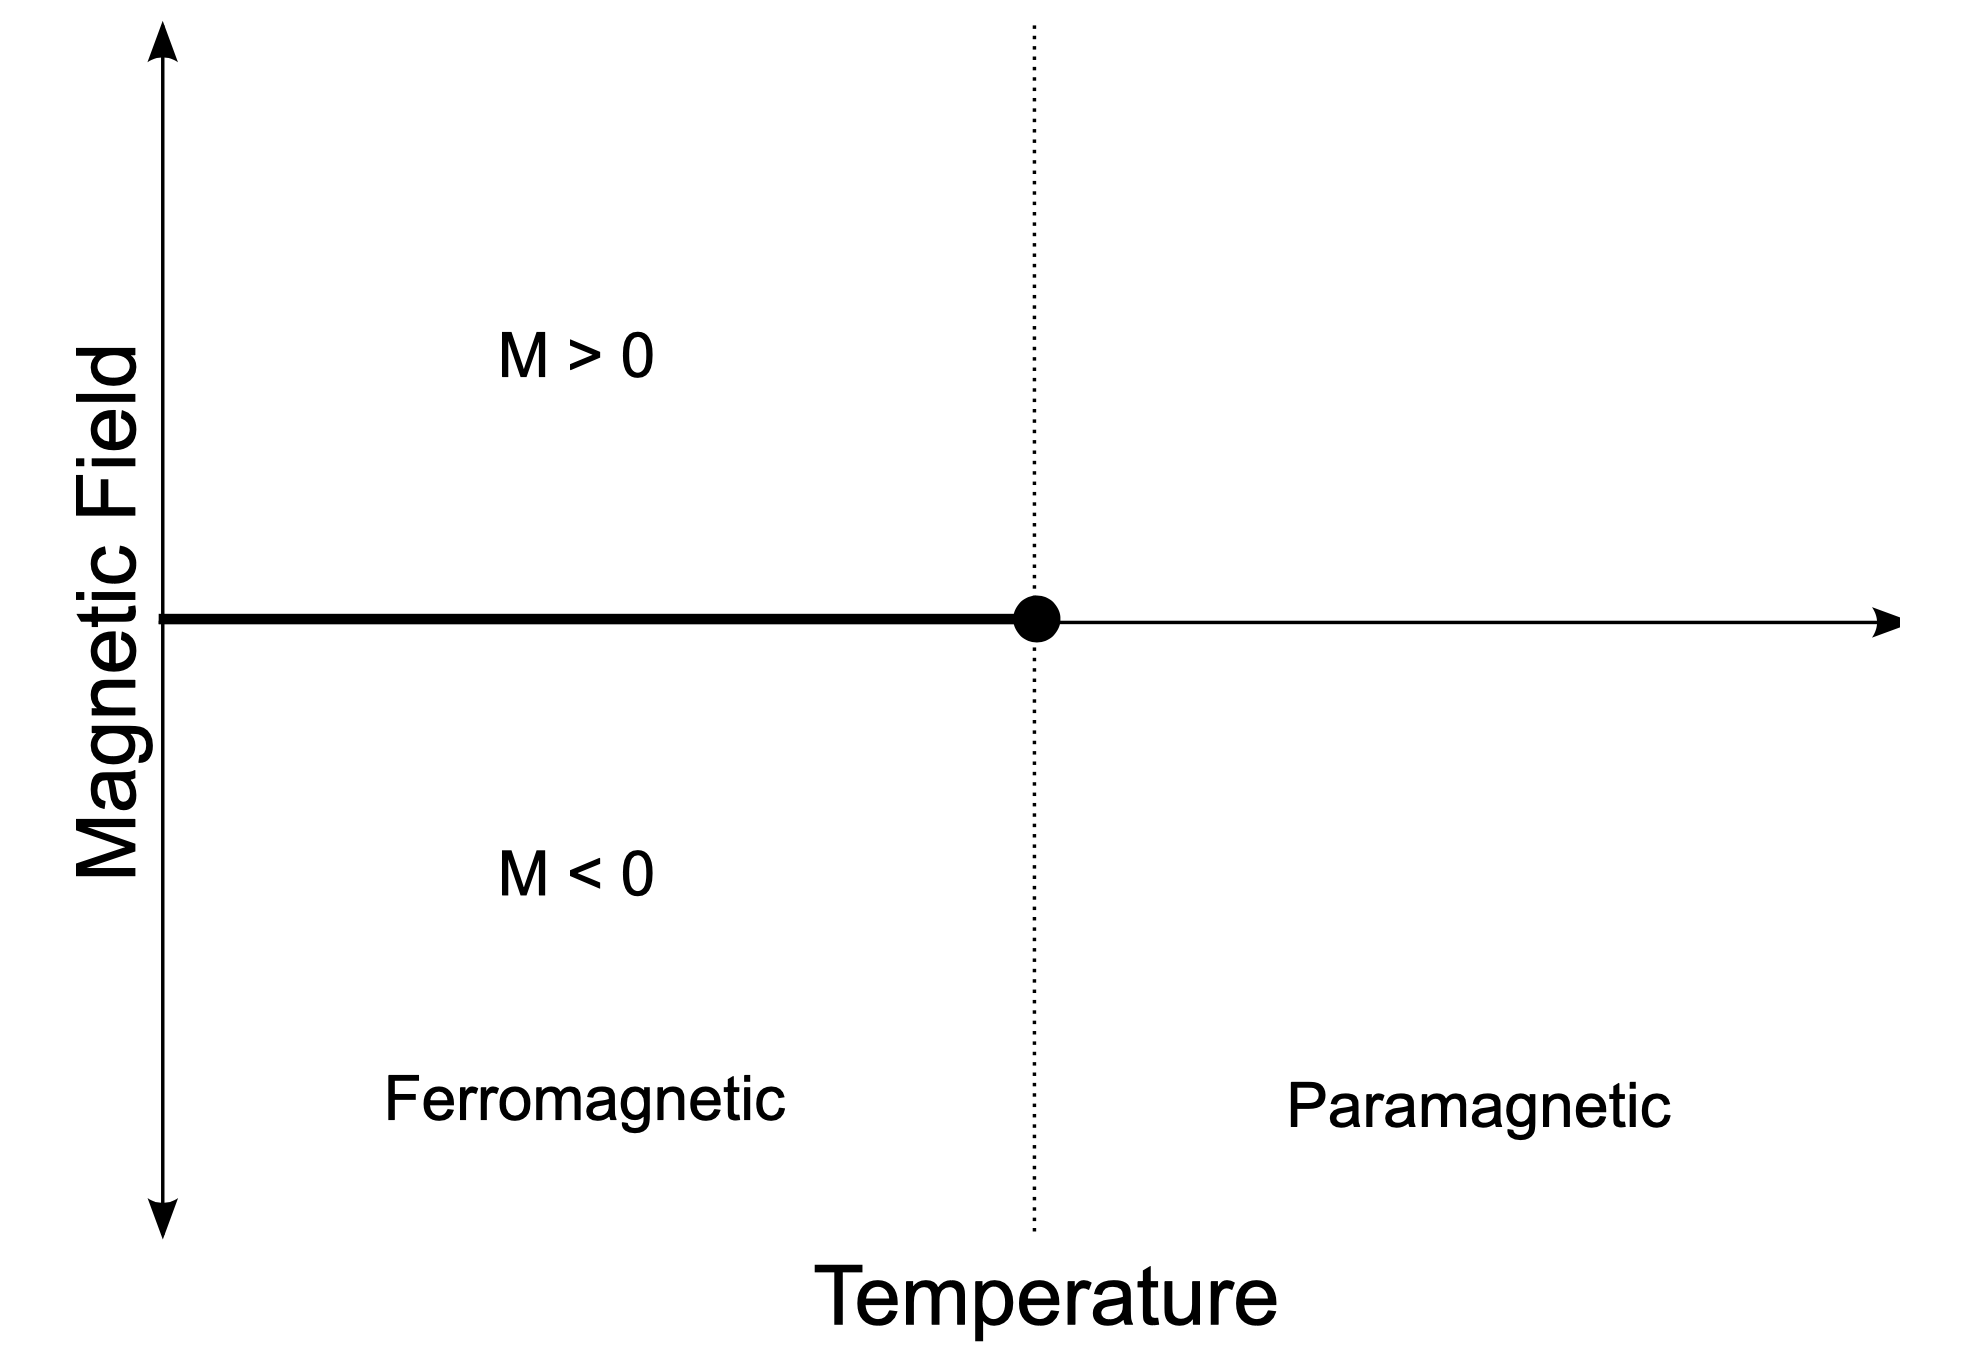
\includegraphics[scale=.22]{magnet_phase_diagram.png}
	\end{aligned}$
	\caption[Phase diagram for fluids and uniaxial magnets]{\label{fig: phase diagram}\textbf{(a)} Phase diagram for fluids \textbf{(b)} Phase diagram for uniaxial magnets}
\end{figure}

The phase diagram of a system can be $n-$dimensional: the dimension of the diagram reflects the number of macroscopic parameters to tune with as we move between various phases. In the case of fluids, we have two parameters: \emph{pressure} $P$ and \emph{temperature} $T$. Similarly, if we consider the phase diagram of a uniaxial magnet, it also has two parameters to tune: temperature and \emph{external magnetic field} $h$.\footnote{A uniaxial magnet is a magnet whose magnetization can point in only one dimension, see \figref{\ref{fig:Ising model}}.} Other systems may have phase diagrams of different dimensions; for instance, \cite{wang2015three} models biological structures as thermodynamic systems and classifies morphological patterns arising on the surface of  tissues as various phases; in its application, the resultant phase diagram has three parameters, see \figref{\ref{fig: phase diagram 2}}.

\begin{figure}
	\centering 
	\begin{gather*}
		(a)\begin{aligned}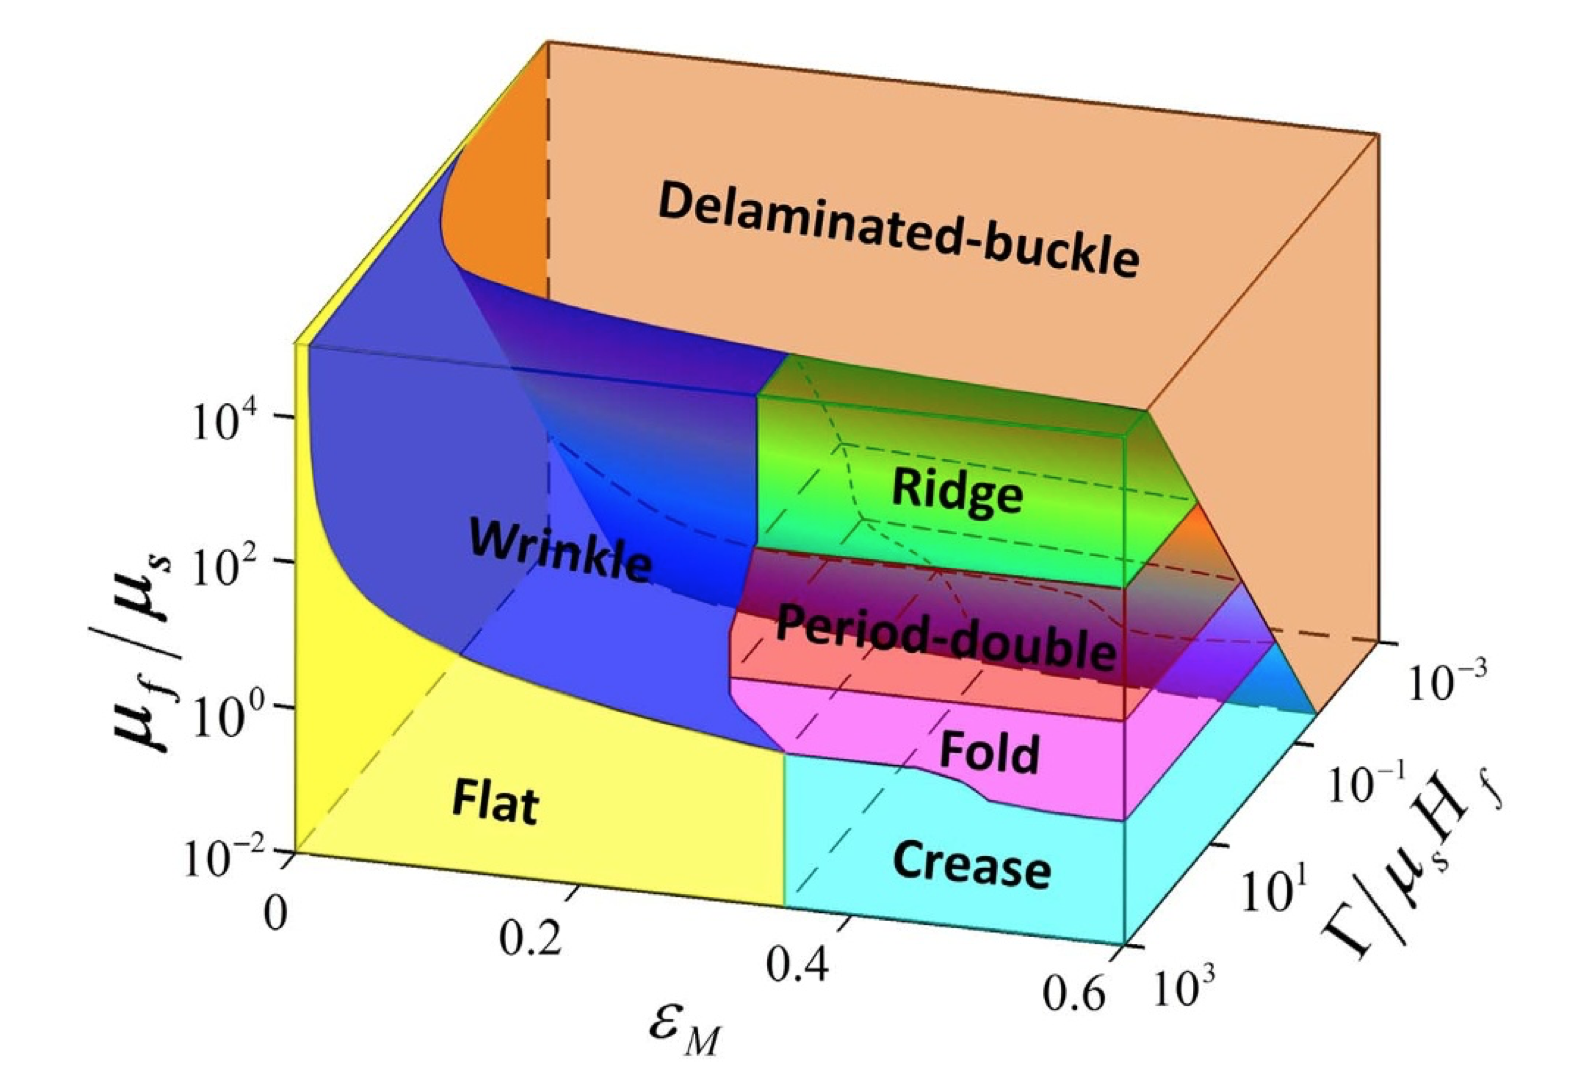
\includegraphics[scale=.315]{phase_diagram3.png}
		\end{aligned}\\(b)\begin{aligned}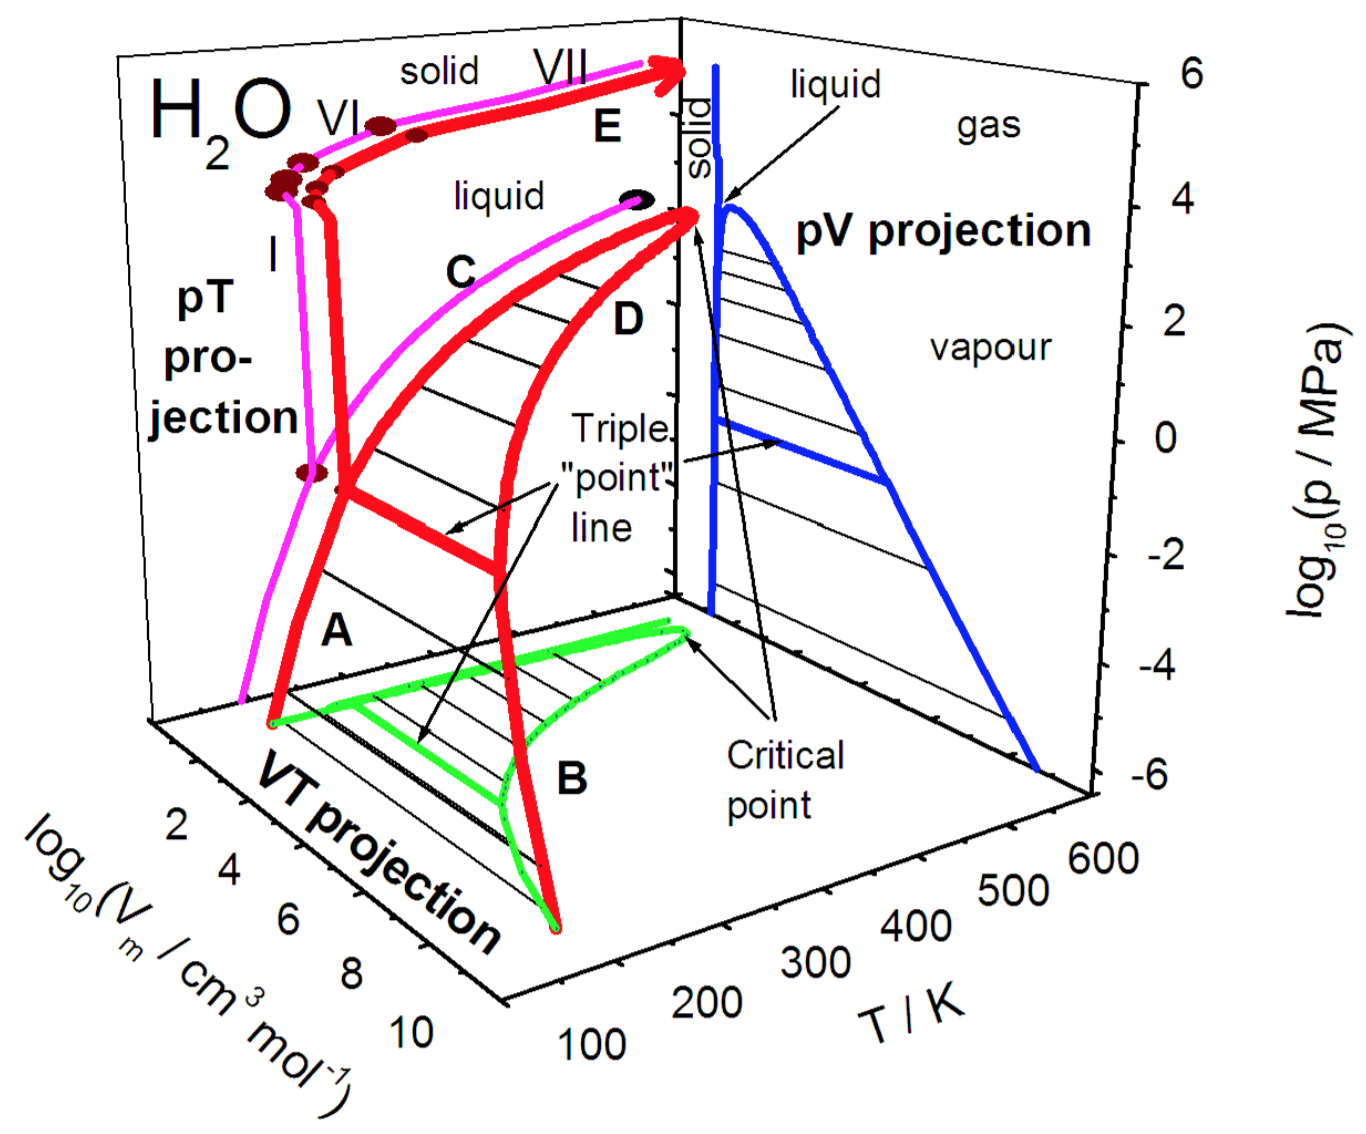
\includegraphics[scale=.315]{phase_diagram4.png}\end{aligned}\quad
		(c)\begin{aligned}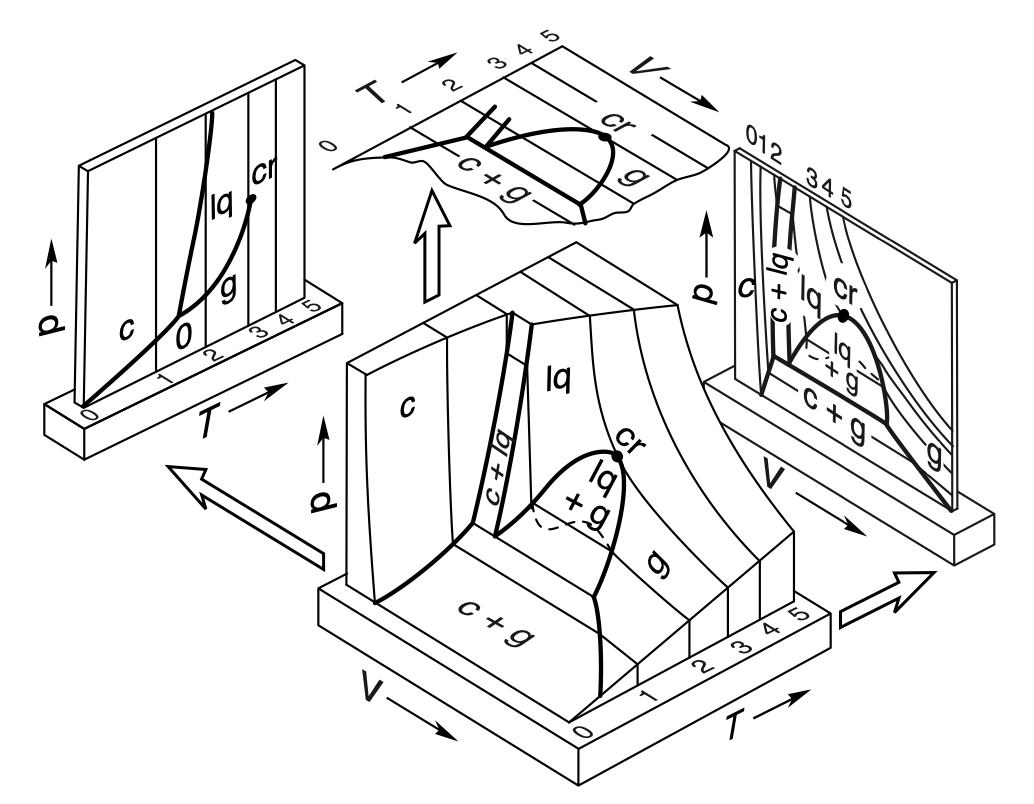
\includegraphics[scale=.42]{phase_diagram5.png}
		\end{aligned}
	\end{gather*}
	\caption[Phase diagrams in three dimensions]{\label{fig: phase diagram 2} \textbf{(a)} A genuine three dimensional phase diagram example: various surface instability patterns induced on biological tissues \cite{wang2015three}. One needs to tune three parameter to sweep all phases. \textbf{(b)} Three dimensional depiction of the phase diagram of water and its various projections \cite{glasser2004water}: one can still reach all phases by tuning only two parameters.\footnotemark \textbf{(c)} An illustrative orthographic (isometric) three-dimensional pVT diagram of water \cite{glasser2004water}.}
\end{figure}
\footnotetext{See also \hyperref{http://biomodel.uah.es/Jmol/plots/phase-diagrams/inicio.htm}{}{}{http://biomodel.uah.es/Jmol/plots/phase-diagrams/inicio.htm}.}

\begin{figure}
\centering
	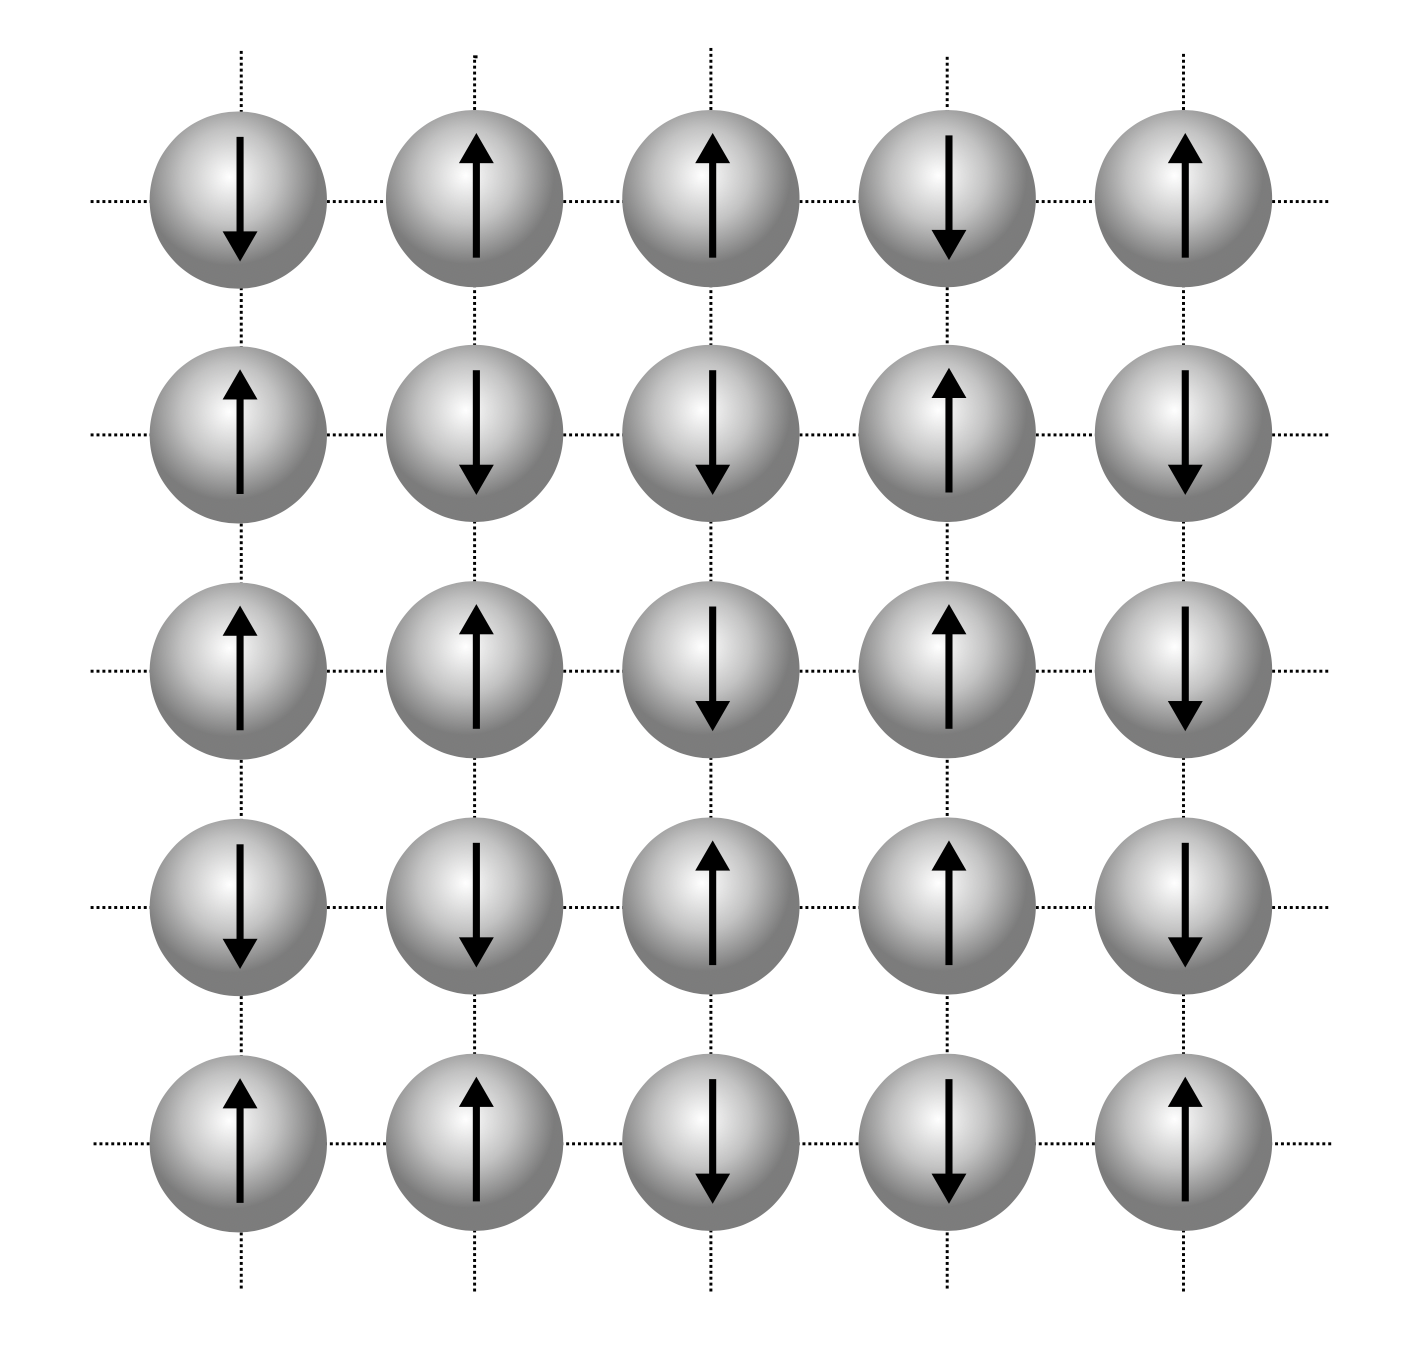
\includegraphics[scale=.3]{Uniaxial_lattice}
	\caption[Uniaxial magnet as a set of one-dimensional spins on a lattice]{\label{fig:Ising model} Uniaxial magnet as a set of one-dimensional spins on a lattice. If we examine this system at macroscopic scales, we do not observe individual spins but rather an average magnetization $M(x)$ which is a continuous field, hence we can describe it with a field theory. On microscopic scales, this theory is described by \emph{the Ising model}.}
\end{figure}


One can \naively think that we can always change the dimension of the phase diagram by considering other parameters; for instance, for fluids, we can also consider \emph{molar volume} $V$ as a parameter: the resultant graphical depiction of the phase diagram, along with its projection to various planes, can be seen in \figref{\ref{fig: phase diagram 2}}. It is true that such depictions can be quite useful, and one might conclude then that the phase diagram is in general of arbitrary dimension, as we can add more and more directions of arbitrary parameters. However, \emph{what we mean by the dimension of the phase diagram} is the number of parameters \emph{necessary} to tune to sweep all different phases. In the case of fluids, two parameters are sufficient to go over all phases, so we say that the phase diagram of fluids is two-dimensional, so is that of uniaxial magnets.

The dimension of the phase diagram, as a global property, may not be as so useful as \emph{the dimension of the fixed points}, i.e. the number of parameters one needs to tune to reach a fixed point in the RG (renormalization group) framework. This is a local property, because it may differ from one fixed point to the other in the same phase diagram. In fact, the number of parameters necessary to reach a \emph{critical fixed point} is same as the number of \emph{relevant operators} (operators whose scaling dimension is less then the spacetime dimension \label{page: first instance of relevant operators}) in the \emph{conformal field theory} which describes that critical fixed point -- more on that below! Note that we do not require knowledge of RG framework in these notes, so please remain comfortable if you are unfamiliar with it. 

Before we dive into critical fixed points or conformal field theories, let's take a step back and try to understand the phase diagrams in \figref{\ref{fig: phase diagram}}: they consist of some regions (bulk phases), lines dividing those regions (phase transitions), and endpoints of some lines (critical points).  From statistical mechanics point of view, the phase diagram consists of \emph{non-analyticities} of the free energy\footnote{For those who have difficulty remembering their stat-mech courses, the free energy is the ultimate function from which all thermodynamic quantities can be derived via differentiation. I'll be rather ambiguous and do not specify \emph{which} free energy I refer to (Helmholtz, Gibbs, Landau, etc.), because it will not matter for the qualitative discussion.} in thermodynamics limit,\footnote{Remember that the free energy $F$ is given as 
\be 
e^{-\b F}=\Tr e^{-\b H}
\ee 
for $\b\equiv (k_B T)^{-1}$ where $k_B$ is the Boltzmann's constant and $T$ is the temperature. $H$ is the Hamiltonian and the trace denotes a sum over all degrees of freedom mentioned in $H$. The partition function $Z$ is analytic as the Hamiltonian is usually an analytic function and a \emph{finite} sum of analytic functions is itself analytic, as long as the trace operation is a summation of \emph{finitely many} degrees of freedom. Hence, the phases and phase transitions only appear in the thermodynamic limit, where the degree of freedom becomes infinite and the trace usually turns into a \emph{path integral}.
} but actual computation of the free energy is almost always impossible so we do not have a clear handle on the derivation of the phases from the microscopic theory: in fact, the full phase diagram of a substance \emph{can not be computed in general} starting from the microscopic theory! This is not because of our lack of knowledge or of a small technical problem, but  of \emph{the undecidable nature of the mathematical problem itself}!\footnote{
\label{footnote: decidability}
Here by undecidable we mean that a general algorithm which is guaranteed to solve this problem in finite time cannot be found; see \cite{bausch2021uncomputability} for the case of phase diagrams. I highly recommend ``Math Has a Fatal Flaw'' video of the Youtube channel \emph{Veritasium} for a broader view of the mathematical issue undecidability, along with incompleteness and inconsistency problems.
} In short, we have the general formula but it will not do any good for us if we insist on computing the phases from the microscopic theory.

Let us instead construct a \emph{phenomenological} model for the free energy.\footnote{The term ``phenomenological'' needs a little bit explanation. I use it the same way Goldenfeld uses in \cite{Goldenfeld:1992qy}. He has a beautiful explanation there and I would like to copy/paraphrase/edit some part of it here.

\emph{In constructing physical theories, we always use a certain level of description. Thus, in describing the long wavelength behavior of a magnet, we write down equations for the coarse-grained magnetization (here, coarse-grained means that the parameter is smoothed out below a certain detail). In describing the motion of a fluid, we write down equations of motion for the velocity field $v(r,t)$; however, the velocity field is actually a coarse-grained velocity of many particles in a small volume element in the neighborhood of the point $r$. In these and other examples, the variables of interest are always defined with respect to some coarse-graining process so that phenomena below some scale are subsumed somehow into the equations for the coarse-grained variables of interest. }

\emph{In a phenomenological description of a system, we try to describe the behavior solely in terms of the coarse-grained variables, without reference to the microscopic physics on scales shorter than the coarse-graining length. Inevitably, the description of the coarse-grained variables introduces other parameters; for example, in a magnet, the parameters of the Landau free energy, or in a fluid, the coefficient of viscosity. These phenomenological parameters are determined by the microscopic physics: for example, the viscosity of a fluid may be calculated, with some approximation, from kinetic theory. A successful phenomenological theory contains only a finite number of such parameters (the smaller the better), and does not attempt to calculate the phenomenological parameters. These are taken to be inputs to the theory.}

\emph{How does a phenomenological theory change when the microscopic physics is altered? From the above, the only possible change can be in the values of the phenomenological parameters. If new phenomenological parameters have to be introduced whenever the microscopic physics is changed, then the theory is not, by definition, phenomenological! In this sense, a successful phenomenological theory should be insensitive to the changes in the microscopic physics, although the phenomenological parameters may change.
}

\emph{An interesting corollary of this discussion is that all our physical theories are phenomenological, because in principle there may always be more degrees of freedom in finer and finer details!}} For that, we consider the free energy as a function of various phenomenological variables $K_i$ and write
\be 
\label{eq: landau potential in path integral}
e^{-\b F(K_i)}=\int \cD\f e^{-\b L(K_i,\f)}
\ee 
where $\int \cD\f$ denotes a path integral over the field $\f(x)$ which represents the degrees of freedom in the theory (Knowledge of path integrals is not essential for the discussion so just think of it as an ordinary integral if you are unfamiliar with the concept.). If we started with the microscopic theory, we would instead have trace over degrees of freedom, which would potentially include discrete sets (such as spins on lattice sites), but as we are constructing a \emph{phenomenological model}, we are coarse-graining the microscopic details and representing the degrees of freedom by a continuous field $\f(x)$.

The $L(K_i,\f)$ is an arbitrary function for now, which would be the Hamiltonian in the microscopic theory. To leading order, we can assume that the dominant contribution to \equref{eq: landau potential in path integral} comes from the form of $\f(x)$ which minimizes $L(K_i,\f)$, hence we have 
\be 
e^{-\b F(K_i)}= e^{-\b L(K_i,\bar\f)}
\ee 
where $\bar\f(x)=\bar\f$ is a uniform field that minimizes $L(K_i,\f)$.

This phenomenological approach can then be summarized as follows:
\begin{itemize}
	\item Determine a measurable macroscopic variable $\f$ which changes over different phases: $\f$ is called the \emph{order parameter}.
	\item Write down an analytic function $L$ of $\f$ in terms of the phenomenological parameters $K_i$. $L$ as a function of $\f$ should have the symmetries of the Hamiltonian.
	\item Minimize $L$ with respect to the variable $\f$: the minimum gives the free energy!
	\item If there is a non-analyticity in taking the minimum, that should give us the phase transition!
\end{itemize}
This approach is called \emph{Landau formalism}, named after \emph{Lev Davidovich Landau}, and $L(K_i,\f)$ is usually called \emph{the Landau potential}.\footnote{Here I simplified the phenomenological Landau theory, interested reader may consult \cite{Goldenfeld:1992qy} for an excellent review.} Physically, Landau formalism is simply an application of the \emph{mean field theory}: we approximate whatever it is of physical interest (such as magnetization field $M(x)$ of a magnet or density field $\rho(x)$ of the fluid) by its mean value and ignore the fluctuations!

Let us illustrate this approach for uniaxial magnets. The relevant parameter here is the magnetization $\vec{M}(x)=M\hat{z}$ of the magnet, which we take to be in the $z-$direction -- note also that it takes its mean value $M$. Then the simplest form of Landau potential we can write down reads as 
\be 
L(K_i,M)=K_0+K_1M^2+K_2M^4-hM
\ee 
which is analytic in $M$ and contains the ferromagnetic coupling of the magnetic field $M$ to the external magnetic field $h$.\footnote{The sign needs to be negative for a ferromagnet so that  parallel $M$ and $h$ decreases the energy, as opposed to antiferromagnets coupling $+hM$.} We note that the truncation of higher order terms (such as $M^6$) is not warranted in general, however it is valid as long as Landau formalism itself is applicable to the problem at hand.\footnote{\label{footnote: upper critical dimension}In short, the Landau formalism is a sufficient description only above an \emph{upper critical dimension}; physically, ignored fluctuations become important if the spacetime dimension is not high enough: for uniaxial magnets, the upper critical dimension is $4$. If we are above the upper critical dimension, then the truncation of higher order terms, i.e. $M^6$, is appropriate because their contribution diminishes as we near the critical point. This is actually closely linked to the \emph{renormalization} of quantum fields and suppression of irrelevant terms as the energy scale tends to infinity. \draftnote{Maybe I can put more explanation here or even show how this is true, i.e. $t$ versus $\Lambda^{-1}$.}}

As $K_0$ simply shifts the free energy, we can discard it.\footnote{Observable quantities such as susceptibility are derivatives of the free energy.} Likewise we can rescale $M$ to absorb $K_2$ (which needs to be a positive number for $L$ to have a minimum), hence we have
\be 
\label{eq: Landau potential}
L(a,M)=aM^2+M^4-hM
\ee 
which gives the free energy by minimization:
\be 
\{\bar M,F(a,h)\}=\left\{\begin{aligned}
\left\{-\frac{h}{2a},-\frac{h^2}{4a}\right\}+H.O.T.\qquad a>0\\
\left\{\pm\sqrt{\frac{-a}{2}},-\frac{a^2}{4}\right\}+H.O.T.\qquad a<0
\end{aligned}\right.
\ee 
where we wrote down the result for weak external magnetic field $h$ for simplicity, and $H.O.T.$ refers to terms higher order in $h$.

It can be checked by looking at the full form of the result that the function is analytic unless $h=0$. If $h=0$, then there is a cusp at $a=0$, i.e. second derivative of $F(a)$ has a discontinuity at $a=0$. And for $a<0, h=0$, there are in fact two minima of the Landau potential, hence two possible choices for the magnetization. We can summarize these findings as follows:
\begin{enumerate}
	\item There is no phase transition unless $h=0$ (F(a,h) is analytic there)
	\item There are two minima of the Landau potential for $a<0$ if $h=0$: we have a \emph{spontaneous symmetry breaking}. Physically, this means for $h=0$ that there is no magnetization if $a$ is positive and there is a magnetization $M\ne 0$ if $a$ is negative but the sign of $M$ can be either $\pm$. So we have the \emph{disordered phase} for $a>0$ and \emph{ordered phase $a<0$}, and there is a phase transition at $a=0$ as $a$ is varied at $h=0$.
	\item For $a<0$, we have a degeneracy among the minimum at $h=0$, but if we change $h$ the degeneracy is lifted. Hence, if we keep $a<0$ fixed and vary $h$ from $h>0$ to $h<0$, the minimum jumps from $M>0$ to $M<0$: there is a non-analyticity for the whole line $a<0$ at $h=0$!
	\item The first derivative of the free energy is discontinuous in $h$ at $h=0$ for any value of $a<0$: the phase transition associated with this whole line is called \emph{first order phase transition}!
	
	\item The free energy and its first derivative are continuous at $a=0$, $h=0$: it is the second derivative that brings the non-analyticity when we change $a$. Hence we call the associated phase transition a \emph{continuous phase transition}!\footnote{In the literature, such a transition is also called a \emph{second-order phase transition}. This follows from Paul Ehrenfest's classification of phase transitions: he proposed that \emph{phase transitions could be classified as $n^{\text{th}}$ order if any $n^{\text{th}}$ derivative of the free energy with respect to any of its arguments yields a discontinuity at the phase transition}. This classification is incomplete because there are thermodynamic quantities such as the specific heat that actually diverge at some phase transitions rather than exhibiting a simple discontinuity as the Ehrenfest classification implies. Thus, we will take a more modern approach and classify phase transitions as \emph{first-order} or \emph{continuous} as we did above.}
\end{enumerate}
The situation is best understood with the aid of visuals, so please refer to \figref{\ref{fig: landau potential and phase transitions}}.

\begin{figure}
	\centering 
	\begin{gather*}
	(a)\begin{aligned}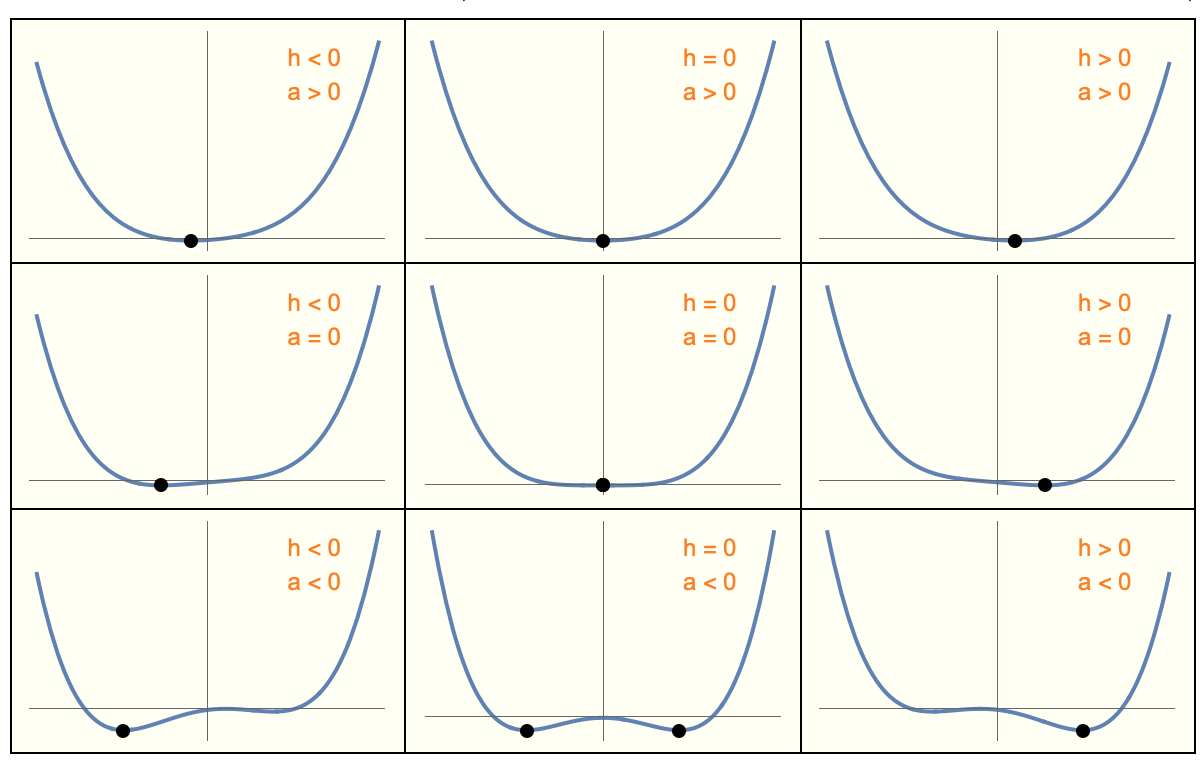
\includegraphics[scale=.7]{Landau_potential.png}
	\end{aligned}\\(b)\begin{aligned}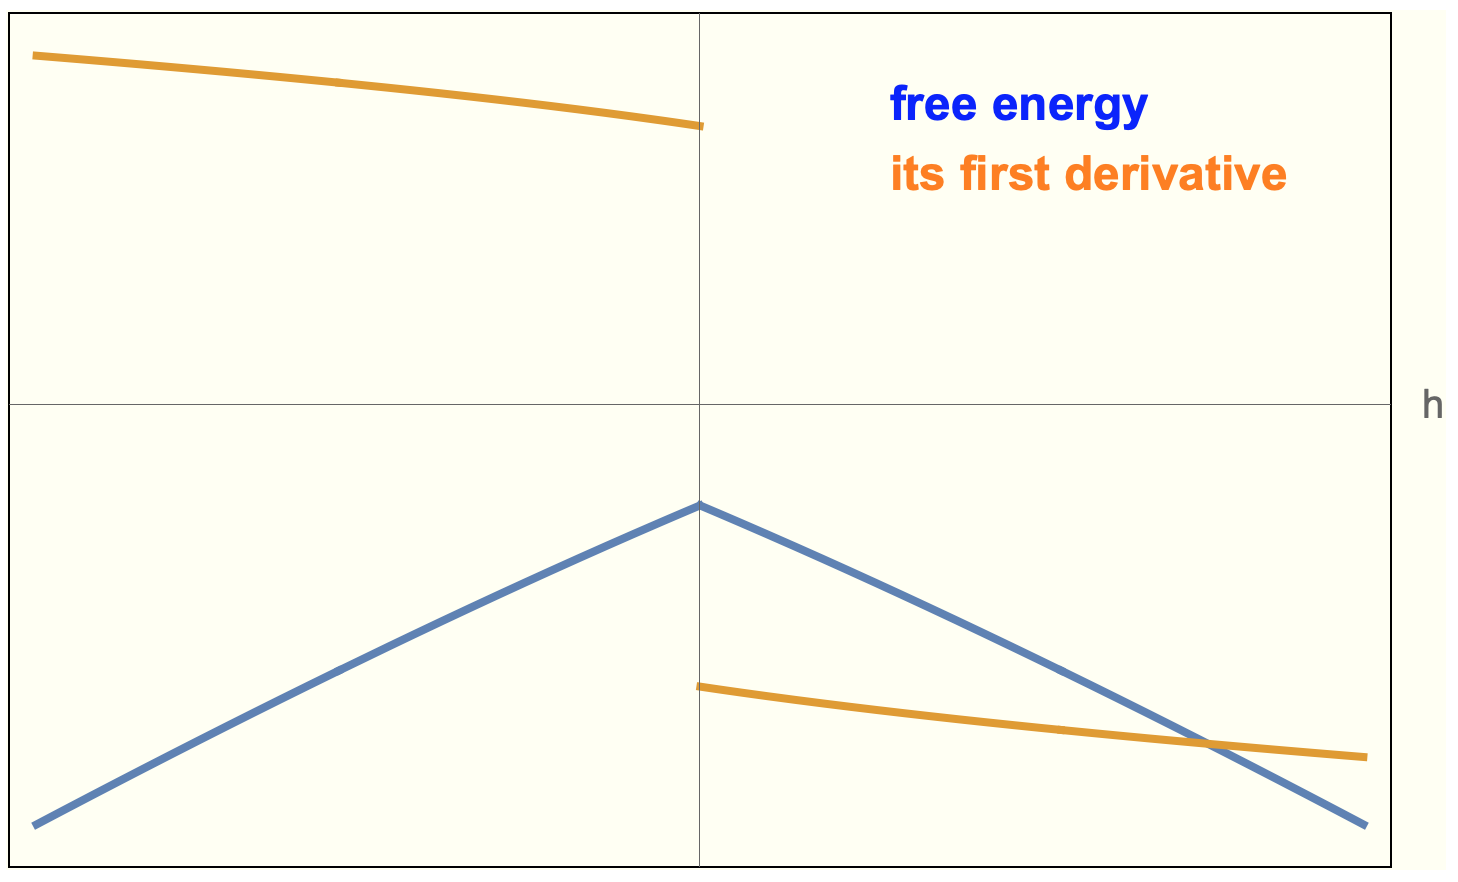
\includegraphics[scale=.28]{first_order_phase_transition.png}\end{aligned}\quad
	(c)\begin{aligned}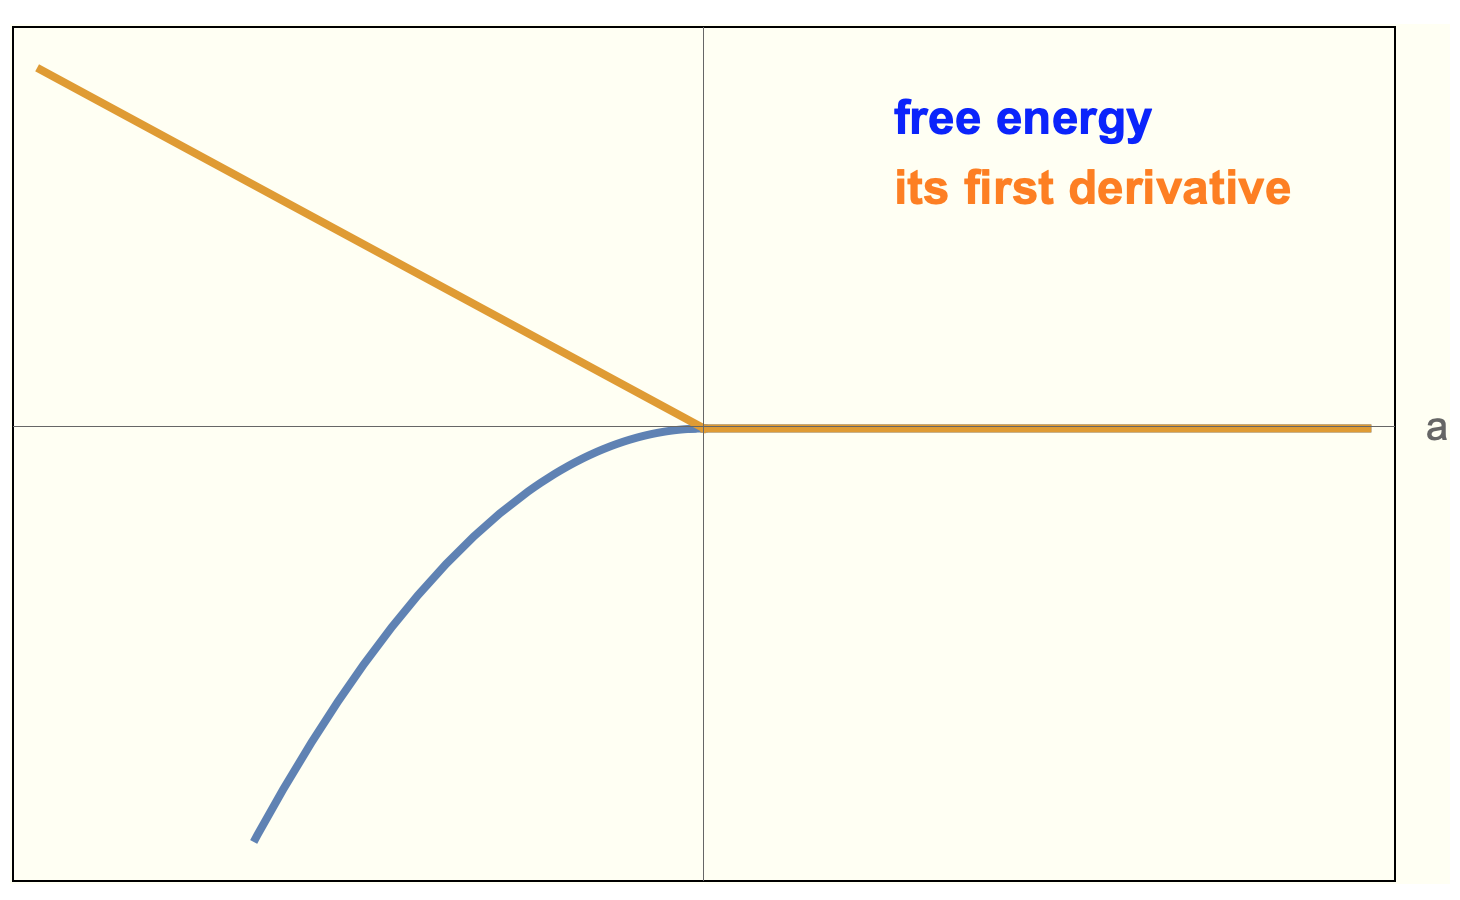
\includegraphics[scale=.28]{continuous_phase_transition.png}
	\end{aligned}
\end{gather*}
	\caption[Phase transitions in the Landau formalism]{\label{fig: landau potential and phase transitions}\textbf{(a)} The Landau potential $a M^2+M^4-hM$ and its minima with respect to the magnetization $M$ for various values of the phenomenological variable $a$ and the external magnetic field $h$. We see that there is no ordered phase at $h=0$ if $a\ge 0$, i.e. the minimum is at $M=0$. If there is  external magnetic field, i.e. $h\ne 0$, then there is a net magnetization $M$ which has the same sign as $h$ as we have the ferromagnetic coupling $-h M$. On the other hand, we still have a net magnetization $M$ even if $h=0$ as long as $a<0$; however, the minima are degenerate so we get a \emph{spontaneous symmetry breaking}, i.e. $M$ can take either positive or negative sign. However, even an infinitesimal $h$ lifts the degeneracy so the minima \emph{jumps} from one value to the other if $h$ is changed continuously from $h<0$ to $h>0$ at $a<0$ (this corresponds to the movement over last column): as the minimum moves discontinuously, we have an associated \emph{first order phase transition}. On the contrary, if we move from $a>0$ to $a<0$ at $h=0$ (this corresponds to the movement over middle row), the minimum changes from zero to a nonzero value continuously: there is a \emph{continuous phase transition} at $a=h=0$. \textbf{(b)} The landau potential at constant $a<0$ as a function of $h$. We see that its first derivative has a discontinuity, showing that the phase transition is indeed \emph{first-order}. \textbf{(c)} The landau potential at constant $h=0$ as a function of $a$. We see that both the function and its first derivatives are continuous, hence the phase transition is indeed \emph{continuous}.
}
\end{figure}

We would like to note that Landau formalism is actually incorrect for $d\le 4$ --- see footnote~\ref{footnote: upper critical dimension} --- and we should not use it for anything quantitative. However, the picture it depicts is actually qualitatively correct: if we take that the phenomenological constant $a$ to have a dependence \mbox{$a\sim T-T_c$}, the phases and the phase transitions described in \figref{\ref{fig: landau potential and phase transitions}} indeed matches the empirical phase diagram in \figref{\ref{fig: phase diagram}}.

\subsubsection{Universality, critical opalescence, and critical exponents}
Why did we review the phase diagrams in the previous section: what are we trying to achieve? Well, as the author, I'm trying to motivate conformal field theories but we are still not there yet! But if we go back to our original discussion, our motivation was to understand the nature of the phase diagrams, such as those in \figref{\ref{fig: phase diagram}}. We found out that in the case of uniaxial magnets, there is a continuous phase transition at the so-called \emph{critical point} (\mbox{$h=0$}, \mbox{$T=T_c$}) and there is a first order phase transition along the line which connects the critical point to the origin (\mbox{$h=0$}, \mbox{$0\le T< T_c$}). We might now ask how important our findings are: after all, uniaxial magnets (magnets whose magnetization can point only in $1$ dimension) are highly-idealized and we may \naively complain that these results do not have a wide range of applicability! However, this is simply not true! The description of and around the critical point is actually \emph{universal}, and whatever information we can acquire regarding the critical point of the uniaxial magnet immediately applies to the critical point of most fluids! This concept is called \emph{universality} and is related to the fact that \emph{same conformal field theory} describes the critical point of both the uniaxial magnets and the most fluids!

The concept of universality can be best understood in the framework of renormalization group, and we'll review that in the next section. For now, let us focus on the implications of universality instead of deriving it:
\begin{itemize}
\label{items: implications of universality}
	\item Critical phenomena, i.e. behavior observed at and around the critical points (i.e. continuous phase transitions) are \emph{independent} of the microscopic theory! In other words, \emph{local} properties of  different systems around their critical points are same! This is in contrast to the \emph{global} properties, i.e. the whole phase diagram, which varies from system to system!
	\item Critical phenomena depends on the \emph{dimensionality} of the space  and the \emph{symmetries} of the order parameter! In fact, we can define \emph{universality classes} based on these! For example, if the order parameter has $\Z_2$ symmetry,\footnote{$\Z_2$ symmetry refers to \emph{evenness} of a system; for instance, the function $x^2$ has $\Z_2$ symmetry because it is invariant under $x\rightarrow -x$.} then we call that \emph{Ising universality class} (why Ising, more below). For instance, both the density fluctuation $\rho$ of a fluid and the magnetization $M$ of a magnet has $\Z_2$ symmetry and fall under Ising universality class: they have identical critical behavior!
\end{itemize}

To summarize, phase diagrams of numerous materials include critical points which has continuous phase transitions, and the behavior of the system at and around the critical points can be categorized into a handful of different universality classes, which means understanding the critical behavior of one system helps us understand the critical behavior of bunch of irrelevant-looking other systems! \emph{But what exactly are we referring to by critical behavior?}

Let us investigate what happens to a fluid near its critical point: if we start with a constant volume of ethane and heat it, it will become opaque at the critical point! If we keep heating it so that it passes the critical point, it will become transparent again, see \figref{\ref{fig: critical opalescense}}. This phenomenon is called \emph{critical opalescence}. This becoming-opaque-at-critical-point feature is by no means special to ethane: we experimentally observe that fluids at their critical point become opaque in general!

\begin{figure}
	\centering 
	\begin{gather*}
		(a)\quad \begin{aligned}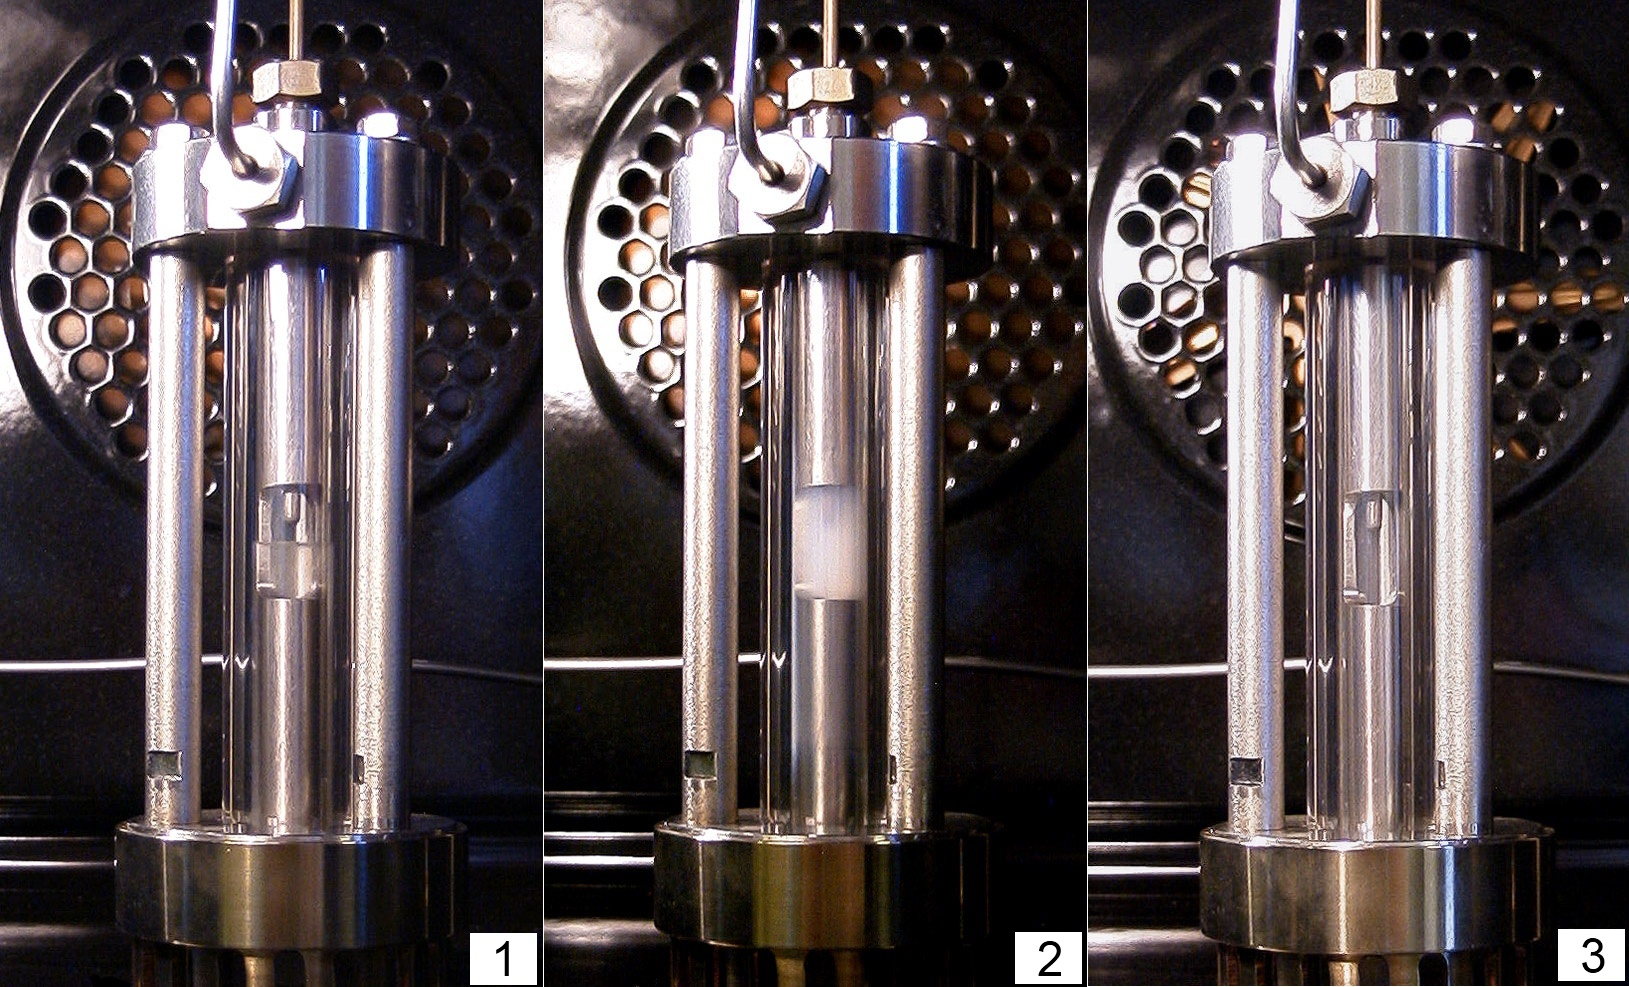
\includegraphics[scale=.8]{CriticalPointMeasurementEthane}
		\end{aligned}\\(b)\begin{aligned}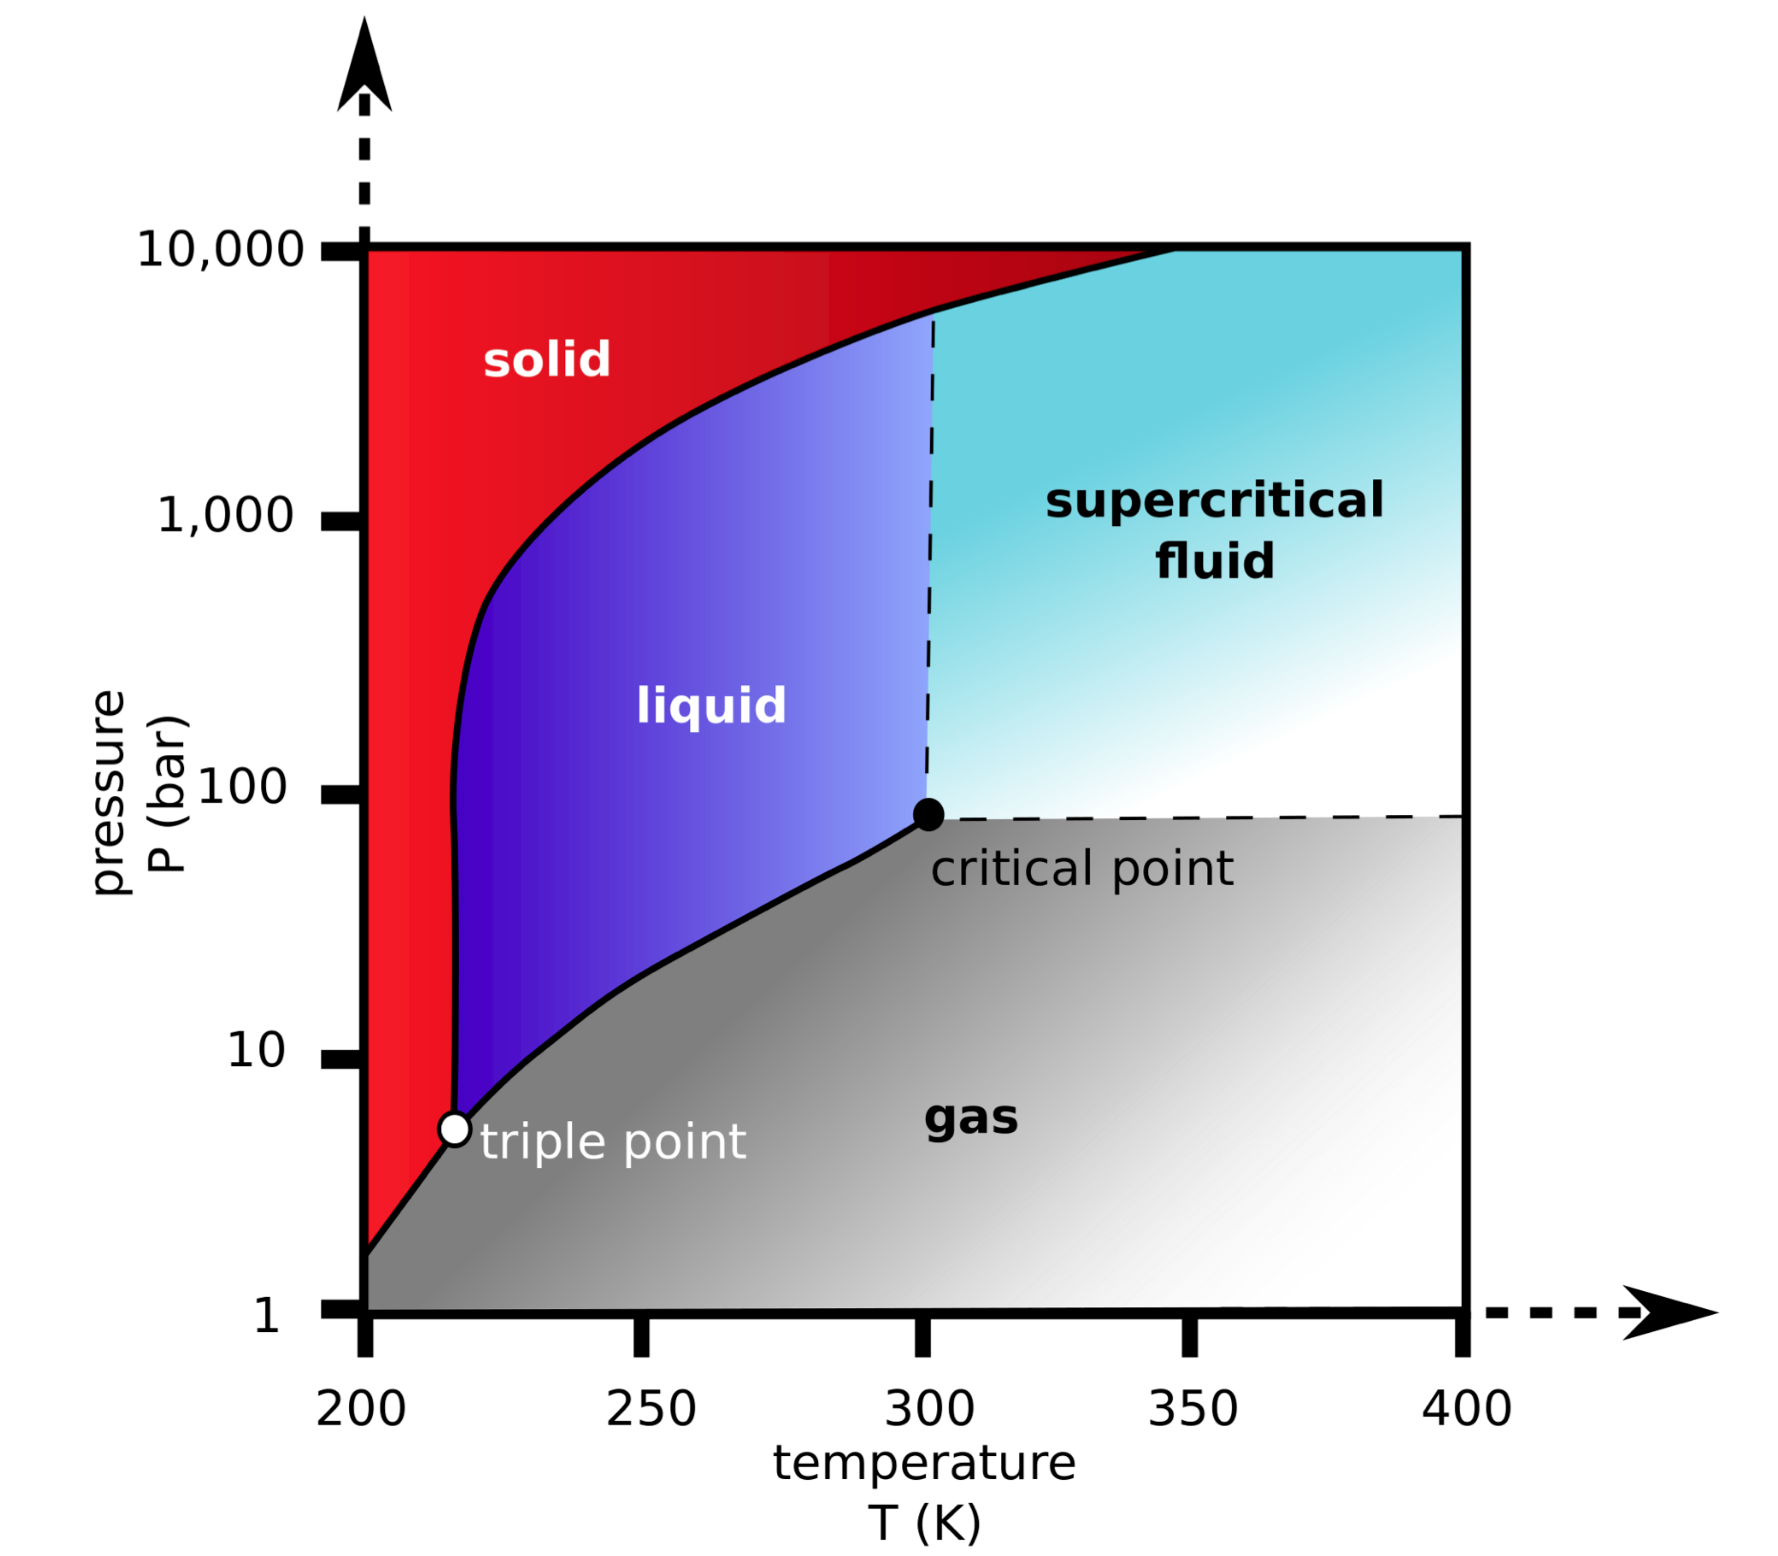
\includegraphics[scale=.2]{phase_diagram.png}\end{aligned}\quad
		(c)\;\begin{aligned}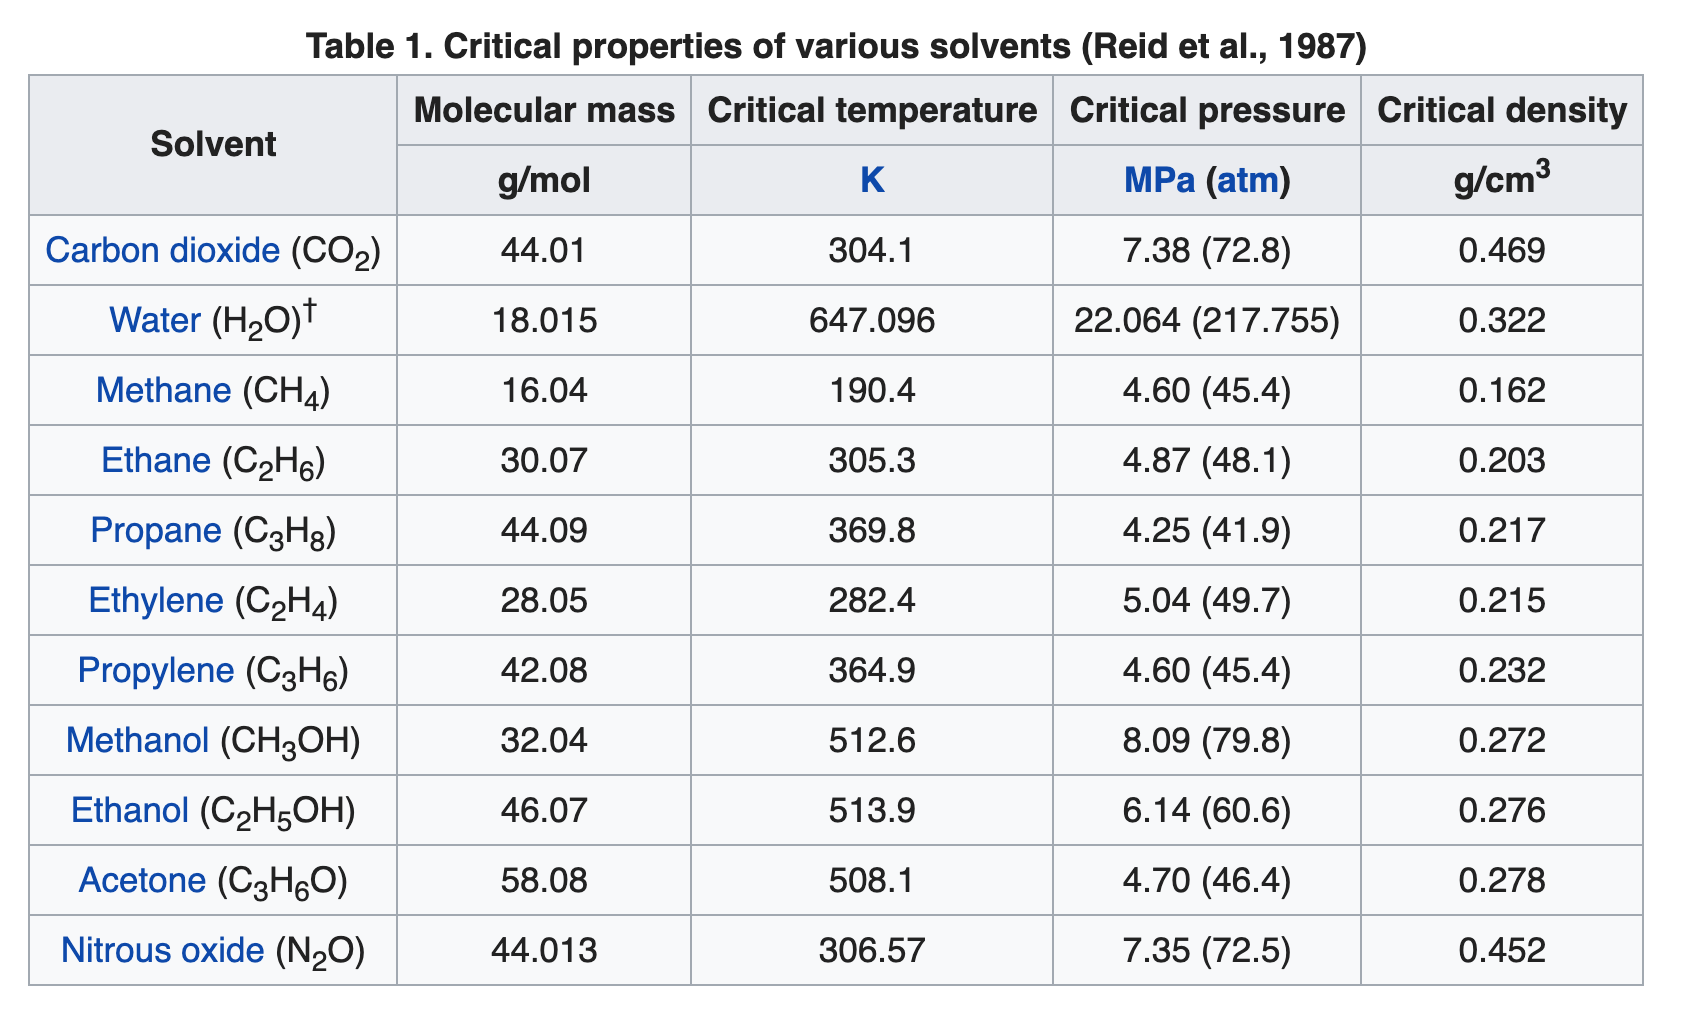
\includegraphics[scale=.3]{critical_table.png}
		\end{aligned}
	\end{gather*}
	\caption[Critical opalescense]{\label{fig: critical opalescense}
		\textbf{(a)} Ethane of constant volume being heated: when it passes the critical point, the critical opalescence is observed, i.e. it becomes \emph{milky}! \textbf{(b)} The critical point for liquids lie at the end of the evaporation line between liquid and gaseous phases. \textbf{(c)} The critical point of various solvents. Despite the difference in critical temperature and critical pressure, the same phenomenon of critical opalescence is observed in all fluids.
	}
\end{figure}

Why is that? At the simplest level, we can understand it intuitively by a phenomenological model of fluids. Let's assume that a scalar field $\rho(x)$ denotes the density of the fluid at position $x$.\footnote{As this is a phenomenological model, we are coarse-graining the microscopic details, so $\rho(x)$ can be thought of as an average density, i.e. number of molecules in the sphere of radius $\Lambda^{-1}$ centered at $x$ divided by the volume of the sphere. If we take $\Lambda\rightarrow0$, $\rho(x)$ becomes a constant and takes its mean value, which gets us back to the mean field theory (i.e. Landau framework). On the other hand if we take $\Lambda\rightarrow\infty$, we get rid of coarse-graining and get back to the microscopic theory (such as a lattice model). The analysis of the effect of the change in $\Lambda$ is precisely the RG framework which we will review in \secref{\ref{sec: review of RG}}.} By continuity of this field, we expect that the densities $\rho(x)$ and $\rho(y)$ are correlated if $y$ is around $x$: if the fluid is dense at a point $x$, it should be dense in its neighborhood as well.\footnote{Technically, there can be a considerable density difference between a point and its neighboring points: maybe a droplet has been spontaneously formed, or a density ripple has just passed. However, such changes depend on time and we are looking at \emph{equilibrium} values of the thermodynamic quantities, hence such differences should be averaged out. Of course, one might ask another question: can we get to the equilibrium in the first place? This is a rather important point because equilibration near a critical point is a non-trivial process.  In fact, the time to reach the equilibrium gets larger and larger as we approach the critical temperature: this phenomenon is known as \emph{critical slowing down}! This subtlety is tangential to our main point so we can assume for simplicity that we are \emph{sufficiently close to} the critical point to assume that we are at the critical point for most purposes, yet \emph{sufficiently away from} it so that we could get the equilibrium in a feasible time.} As $y$ gets further away from $x$, we expect the correlation to die down if the interactions in the fluid are short-ranged, hence we expect \emph{the correlation function}\footnote{
	In these notes, we are using Dirac's bra/ket notation in extremely abusive manner! In \equref{eq: correlation length}, it refers to the expectation value with respect to Boltzman weight  $e^{-\b H}/Z$ as the probability; hence, $\<A\>=Z^{-1}\int\cD\f A e^{-\b H[\f]}$ for the partition function $Z=\int\cD\f e^{-\b H[\f]}$. Thus, if $A=\f\f$, it becomes a correlation function of $\f$. Note that in the Landau framework we have the Landau potential $L$ instead of the microscopic Hamiltonian $H$. This path integral form is extremely similar to what we use in high energy physics for quantum fields: there, we use the bra/ket notation for the similar quantity $\<A\>=Z^{-1}\int\cD\f A e^{-S[\f]}$ for the vacuum generating function\footnotemark $Z=\int\cD\f e^{-S[\f]}$ and the Euclidean action $S$ --- note that we are setting $\hbar=1$ in these notes. For Lorentzian signature, we define the path integral through a Wick rotation. 
	
	We will use Dirac's bra/ket notation to denote conformally invariant structures as well, but there will not be any ambiguity: more on this later!
} \footnotetext{
\label{footnote: vaccum generating function}
If you haven't studied quantum field theory yet, the vacuum generating function $Z$ is the function which can be used to compute any correlation function we like (we do this by taking functional derivatives of $Z$). By LSZ formalism, one can then extract scattering amplitudes or decay rates from the correlation functions; in short, full knowledge of $Z$ is sufficient to extract most of what we are interested in computing in high energy physics.}  to have the form
\be 
\label{eq: correlation length}
\<\f(x)\f(y)\>\sim (x-y)^pe^{-(x-y)/\xi}
\ee 
where $\f(x)\equiv\rho(x)-\bar\rho$ is the \emph{fluctuation} in the density field and $\xi$ is called the \emph{correlation length}!\footnote{
It will not be important for the present discussion but let us give some further information on the correlation function $\<\f(x)\f(0)\>$ --- the correlation function $\<\f(x)\f(y)\>$  can be obtained from $\<\f(x)\f(0)\>$  through the translation invariance of it, i.e. $\<\f(x)\f(y)\>=\<\f(x-y)\f(0)\>$.

The exact analytic form of the correlations functions are not known in general (well, blame mathematicians not physicists) and are not really computable unless the model is exactly soluble (which is extremely rare). However, we can compute their asymptotic forms (either in weak coupling or in long distance separation by perturbation theory, or at the critical point by symmetry arguments). For fluids, we have
\bea[eq: two point function for a fluid]
\label{eq: two point function for a fluid - finite xi}
&\<\f(\bx)\f(0)\>\sim\frac{1}{\xi^{d-2}}\frac{e^{-\abs{\bx}/\xi}}{\left(\abs{\bx}/\xi\right)^{(d-1)/2}}\left(
1+\frac{(d-1)(d-3)}{8(\abs{\bx}/\xi)}+\cO\left(\frac{1}{(\abs{\bx}/\xi)^2}\right)
\right) && \text{ as }\abs{\bx}\rightarrow\infty\text{ and }\xi \text{ finite}
\\\label{eq: critical exponent eta}
&\<\f(\bx)\f(0)\>\sim\frac{a^\eta}{\abs{\bx}^{d-2+\eta}}&&\text{ as }\xi\rightarrow\infty
\eea
Here $d$ is the dimension of the space and $a$ is a microscopic length scale (such as lattice spaceing). See \cite{fisher1962theory} for details on the first formula. The second formula is the \emph{definition} of the critical exponent $\eta$: more on this below.

The Fourier transform of the two point function gives the \emph{structure factor} $S(\bk)$ which is proportional to the intensity of the light scattered through an angle $\theta$ off the fluid where $\abs{\bk}=\frac{4\pi}{\lambda}\sin(\theta/2)$ and where $\lambda$ is the wavelength of the incident light. At the critical point, this then means intesity$\sim\abs{\bk}^{\eta-2}$,\footnotemark\;indicating it diverges as $\abs{\bk}\rightarrow 0$ for $\eta<2$, explaining the critical opalescence \cite{Goldenfeld:1992qy}. For a detailed discussion, see \cite{levy2012phase}.
}
\footnotetext{
	This follows from dimensional analysis: \mbox{$
		\int d^dxe^{-i\bk\.\bx}\abs{\bx}^{-d+2-\eta}
		\propto\int\limits_0^\infty \abs{\bx}^{1-\eta}e^{-i\abs{\bk}\abs{\bx}\cos\theta}d\abs{\bx}\propto\abs{\bk}^{\eta-2}\int\limits_0^\infty y^{1-\eta}e^{-iy\cos\theta}dy$}
}

The correlation length is in general a function of the thermodynamic variables, such as the temperature. As we near a critical point by changing the temperature (or whatever the relevant variable is), the correlation length increases: in fact, at the critical point itself, the correlation length becomes infinity. Hence, the interactions in the fluid becomes long-ranged, and the fluctuations become rather strong, scattering various wavelengths of light and turning the substance into an opaque form!

To summarize, while investigating the critical behavior, we found out that the correlation length diverges at the critical point. In fact, we have a whole family of divergent quantities at the critical point, and it would be insightful for us to go over them briefly. However, to understand them better, let us first list what we have defined so far and define further quantities:\footnote{Wikipedia does a good job at defining and listing them, see \hyperref{https://en.wikipedia.org/wiki/Critical\_exponent}{}{}{https://en.wikipedia.org/wiki/Critical\_exponent}.}
\begin{multicols}{2}
	\begin{itemize}
		\item $t$ -- reduced temperature\footnote{When we say reduced for a thermodynamic quantity $x$, we mean $\frac{x-x_c}{x_c}$ where $x_c$ is its value at the critical point, e.g. reduced temperature $t\equiv\frac{T-T_c}{T_c}$.}
		\item $J$ -- source field (e.g. reduced pressure for fluids and the external magnetic field $h$ for magnets)
		\item $f$ -- free energy
		\item $C$ -- specific heat
		\item $\f$ -- order parameter (e.g. reduced density for fluids and magnetization $M$ for magnets )
		\item $\chi$ -- response function (e.g. compressibility for fluids and susceptibility for magnets)
		\item $\xi$ -- correlation length
	\end{itemize}
\end{multicols}

Observable parameters such as specific heat $C$ or compressibility $\chi$ of a fluid are in general complicated functions of thermodynamic variables; however, \emph{they show a universal behavior and diverge near a critical point as a power law:}
\be 
C\propto\abs{t}^{-\a}\;,\quad 
\chi\propto\abs{t}^{-\g}\;,\quad 
\xi\propto\abs{t}^{-\nu}\; 
\ee 
where the exponents $\a,\g,\nu$ are called \emph{critical exponents}!\footnote{
We have actually more critical exponents. If $t<0$, we can also define $\f\propto(-t)^{\b}$. Likewise, if $t=0$, we define $J\propto\f^{\de}$ and $\<\f(\bx)\f(0)\>\propto\abs{\bx}^{2-d-\eta}$ (see \equref{eq: critical exponent eta}).
}$^{,}$\footnote{The critical exponents $\a,\g,\nu$ have different values depending on $t>0$ or $t<0$.} These exponents form the set of parameters that describe the critical behavior.

Earlier, when we looked at the implications of universality in page~\pageref{items: implications of universality}, we stated that the critical phenomena are independent of the microscopic theory and that it depends only on the \emph{universality class} of the substance. What we meant there is precisely the values of these critical exponents: they \emph{are} universal! For instance, we list examples of several fluids whose critical point lie in \emph{Ising Universality Class} in \tabref{\ref{table: critical data of various fluids}}. Despite the wild differences in critical temperature, they all exhibit the same exact behavior around the critical point with the critical exponents
\be 
\label{eq: critical exponents for 3d Ising}
\a\approxeq0.11\;,\quad\b\approxeq0.33\;,\quad\g\approxeq1.24\;,\quad\de\approxeq4.79\;,\quad\eta\approxeq0.04\;,\quad\nu\approxeq0.63
\ee 
Note that these are the critical exponents in three dimensional space, hence are for \emph{3d Ising Universality Class}: universality class does depend on the dimension of space hence these numbers change if we change the dimension of the space.

\begin{table}
	\centering
	\caption[Critical data for various fluids]{\label{table: critical data of various fluids}Data of various fluids for their critical points at the end of liquid-vapor transition}
	\begin{tabular}{llll}
		\hline\hline 
		\textbf{Substance} & $\bm{T_c}$ (K)& $\bm{\rho_c} \;(kg/m^3)$ &\textbf{Source}
		\\\hline
		Deuterium (D$_2$O) & 644 & 356   &{D M Sullivan et al, 2000}
		\\
		Sulfur hexafluoride (SF$_6$) & 219  & 739 & {Haupt et al, 1999}
		\\
		Carbon dioxyde (CO$_2$) & 304 & 468 & {Damay et al, 1998}
		\\
		Difluoromethane (HFC-32) & 351 & 424 & {Kuwabara et al, 1995}
		\\
		Pentafluoroethane (HFC-125) &  339 & 570 & {Kuwabara et al, 1995}
		\\
		Dinitrogen (N$_2$) &126& 314&{Pestak et al,1983}
		\\
		Neon (Ne)&44&484&{Pestak et al,1983}
		\\\hline\hline 
	\end{tabular}
\end{table}

As we stated earlier, the uniaxial magnet at its Curie temperature with zero external magnetic field is also at the critical point described by Ising Universality Class, hence it exhibits exactly the same critical behavior with the same critical exponent. As we show in \figref{\ref{fig: curie temperatures}}, various magnets have different Cruie temperatures, but the divergence they exhibit is same.

\begin{figure}
	\centering
	$\begin{aligned}
		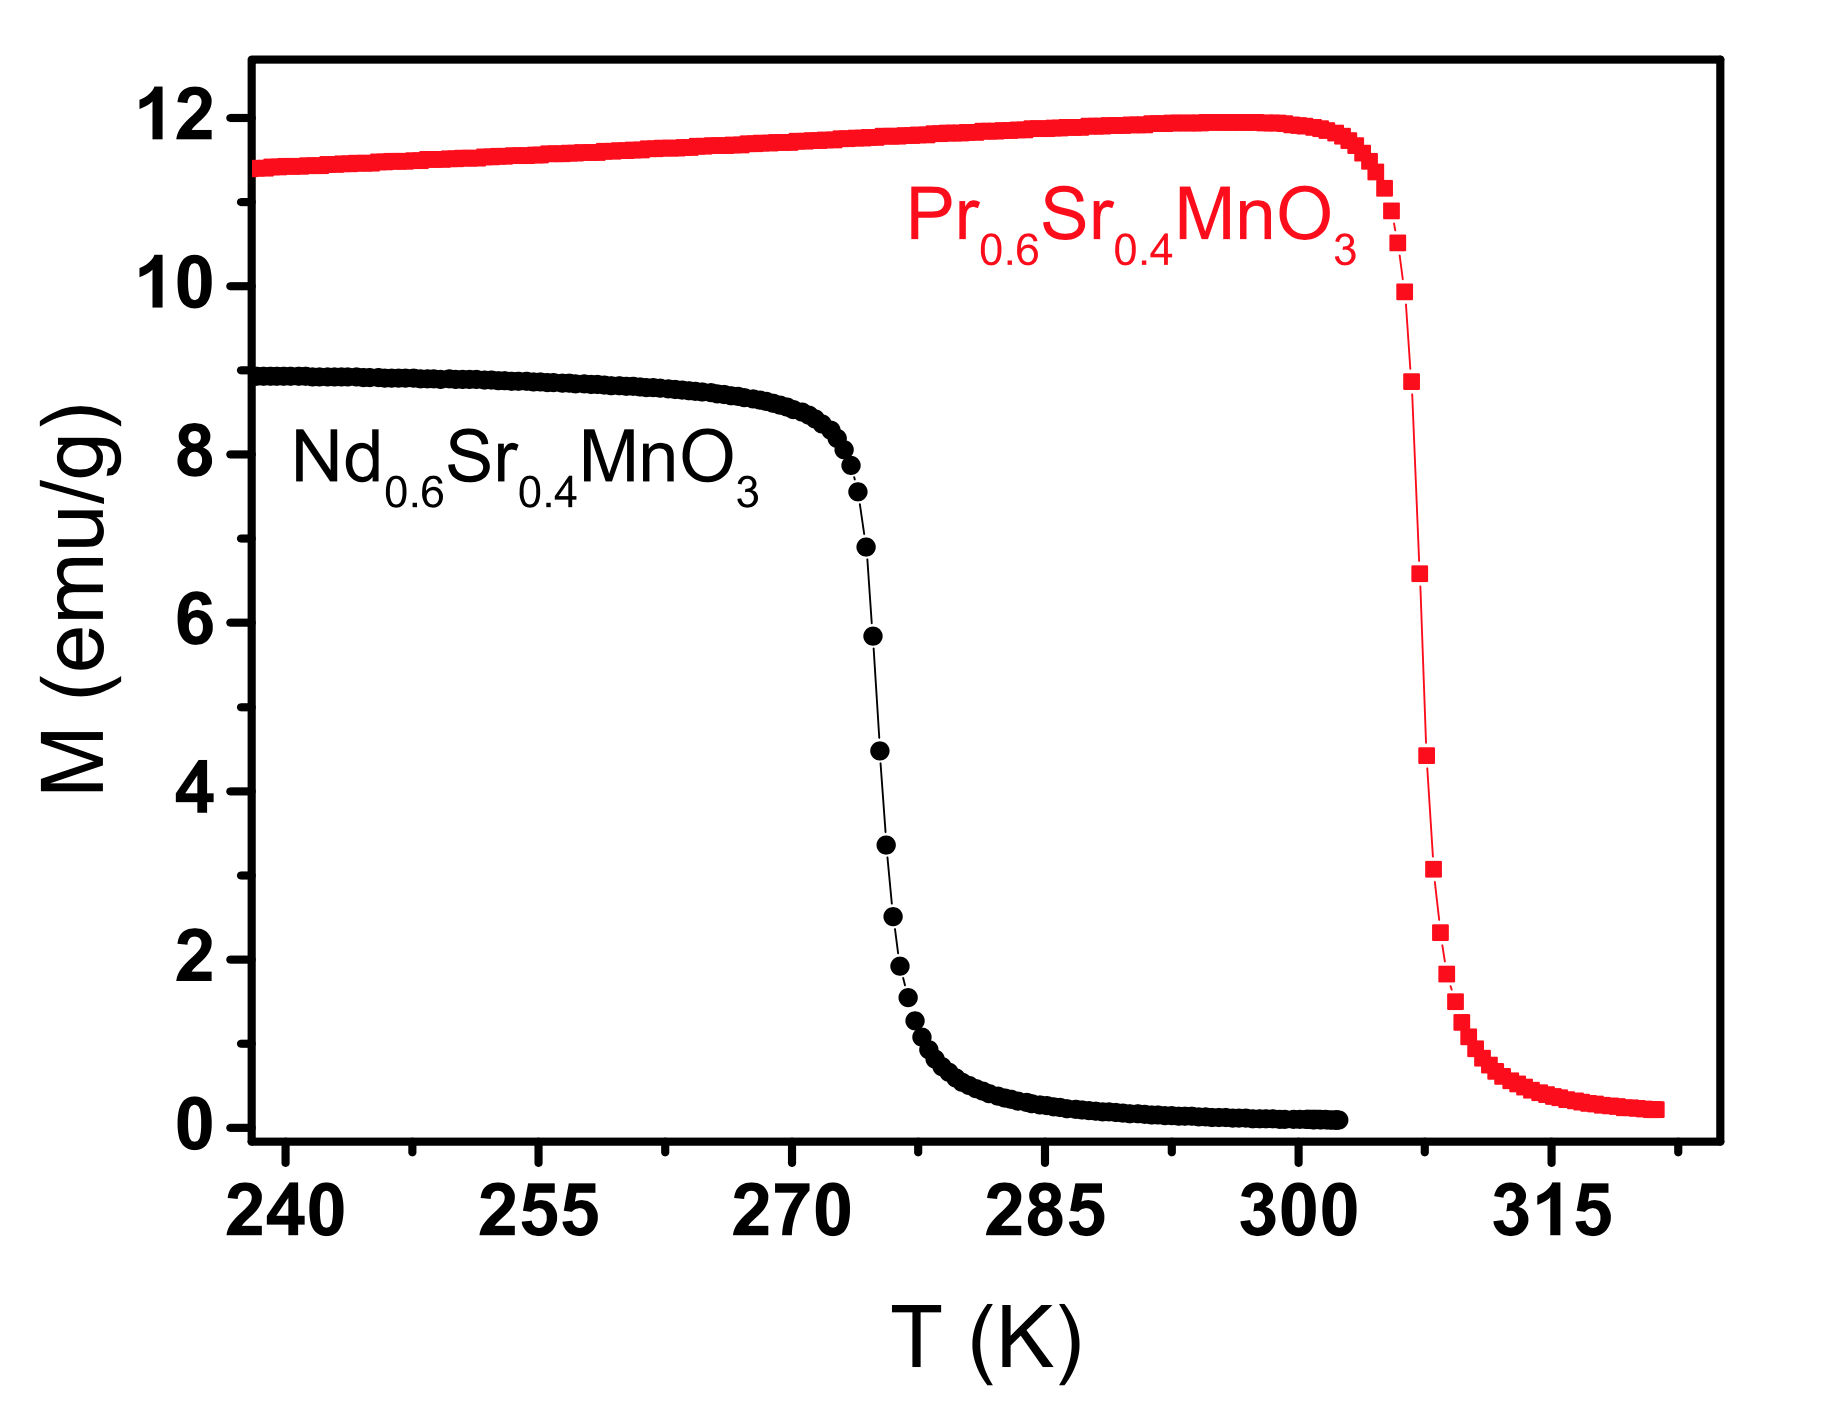
\includegraphics[scale=.22]{magnetGraph1}\\
		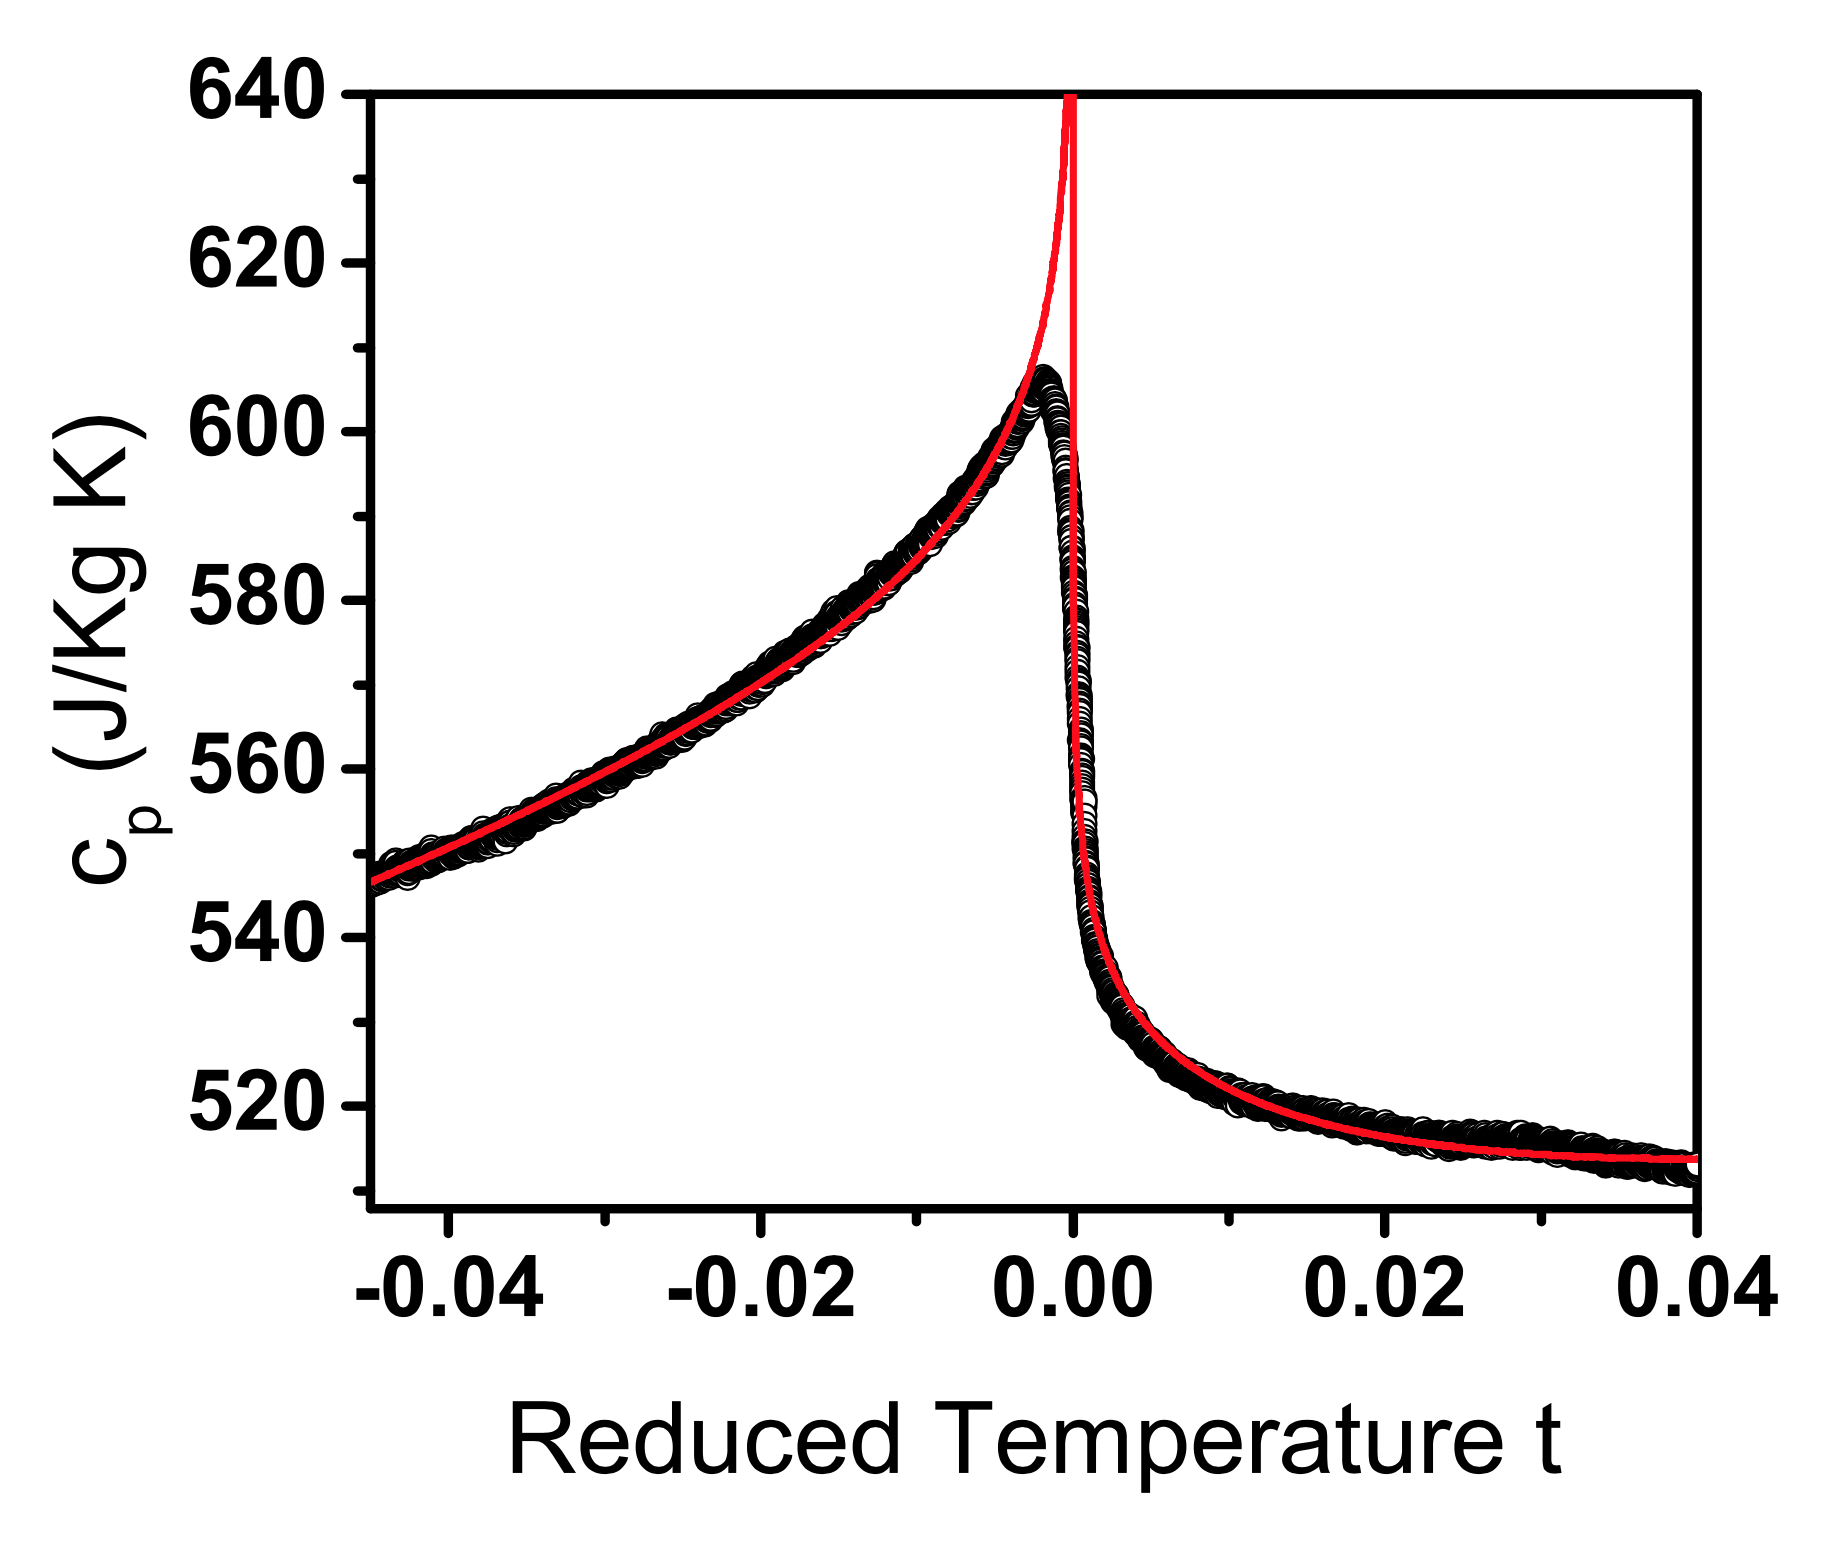
\includegraphics[scale=.22]{magnetGraph2}
	\end{aligned}\qquad\begin{aligned}
		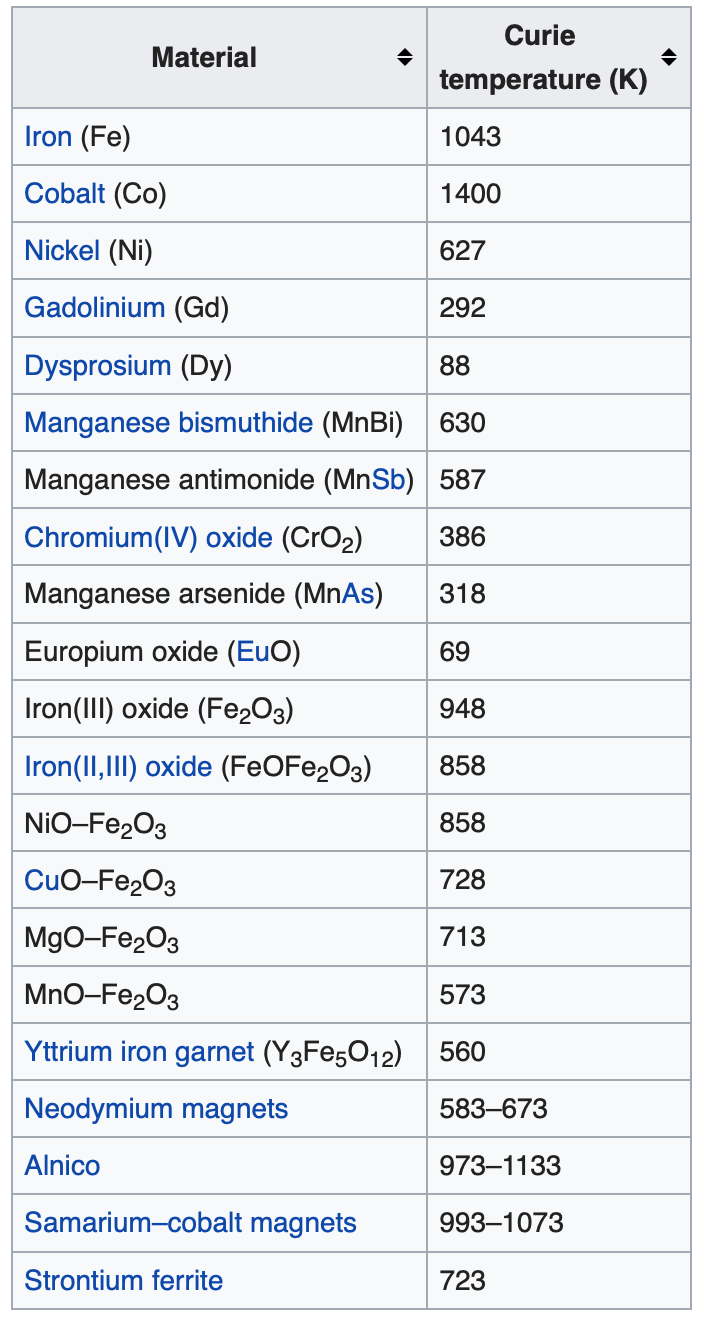
\includegraphics[scale=.5]{Curie}
	\end{aligned}$
	\caption[Uniaxial magnets near their Curie temperature]{\label{fig: curie temperatures}The behavior of magnets near their critical point. On the left, we see the transition from ordered to disordered phase (top) and the divergence of the specific heat (bottom) for magnets in $3d$ Ising Universality Class \cite{oleaga2015three}. On the right, Curie temperature (i.e. critical temperature for magnets) for various magnetic substances are listed, see Wikipedia and the references therein: \hyperref{https://en.wikipedia.org/wiki/Curie\_temperature}{}{}{https://en.wikipedia.org/wiki/Curie\_temperature}.}
\end{figure}

\subsubsection{Summary}
We are now at page~\thepage\;but haven't really motivated why conformal field theories are worth studying in statistical physics, apart from mentioning its name here and there. We will get to that in the next section, but before that, let's finish setting the scene by summarizing our discussion so far.
\begin{itemize}
	\item Matter has different phases (duh!) and all phases can be shown in an $n-$dimensional diagram called \emph{phase diagram} where axes are thermodynamic variables such as temperature, pressure, magnetization, etc.
	\item Phase diagrams have \emph{non-analyticities} in them, which divide them into different regions (phases). These non-analyticities may (but usually do) include a phase-transition which ends at a critical point.
	\item Phase transition lines are usually associated with a \emph{first-order phase transition}, i.e. at least one of the first derivatives of the free energy is discontinuous! Such phase transitions can be explained by spontaneous symmetry breaking, but this \emph{does not have to} be the case! For instance, in magnets, this is the case: above and below the transition line are two different ground states of the potential due to breaking of the $\Z_2$ symmetry in the order parameter (magnetization $M$). In contrast, two sides of the evaporation line in fluids (liquids and gaseous) have the same Euclidean symmetry.\footnote{It is interesting to note that all phases of matter are described by the same microscopic Hamiltonian (and the same partition function), but they may have different symmetries. For instance, in solids, the translation symmetry is broken (atoms are locked in specified positions in a lattice), so the symmetries of the fluid changes over the melting line. As a side note, a corollary of this is that we expect the melting line to extend indefinitely (unlike the evaporation line) because solids have a different symmetry group than liquids and that cannot change analytically! In contrast, liquids and gaseous already have the same symmetry group and it is perfectly fine for the evaporation line to end at a point, i.e. critical point.
}
	\item Critical points at the end of phase transition lines have \emph{continuous phase transition}:\footnote{I'm not sure if there are exceptions, i.e. if there are endpoints of some transition lines where no continuous phase transitions are associated with those points.} the correlation length at such points diverge! The critical \emph{surfaces} does not have to be points (despite we have been talking about critical \emph{points} so far), for instance, in $^{4}$He, there is a superfluid transition along the so-called $\lambda-$line and the phase transition along the whole line is a continuous phase transition, see \figref{\ref{fig: lambda line}}.
	
	\item The behavior of systems around their critical points are independent of the microscopic details of the system but rather on the symmetries and the dimensionality of the space. This in effect divides critical phenemona into \emph{universality classes}: understanding the critical behavior of one system is sufficient to understand the critical behavior of all systems in the same universality class (e.g. understanding the behavior of a uniaxial Nickel magnet at its Curie temperature is sufficient to understand the behavior of compressibility of water or heat capacity of carbon dioxide at their critical points)!
\end{itemize}
In the next section, we will see how these results relate to conformal field theories!

\begin{figure}
	\centering 
		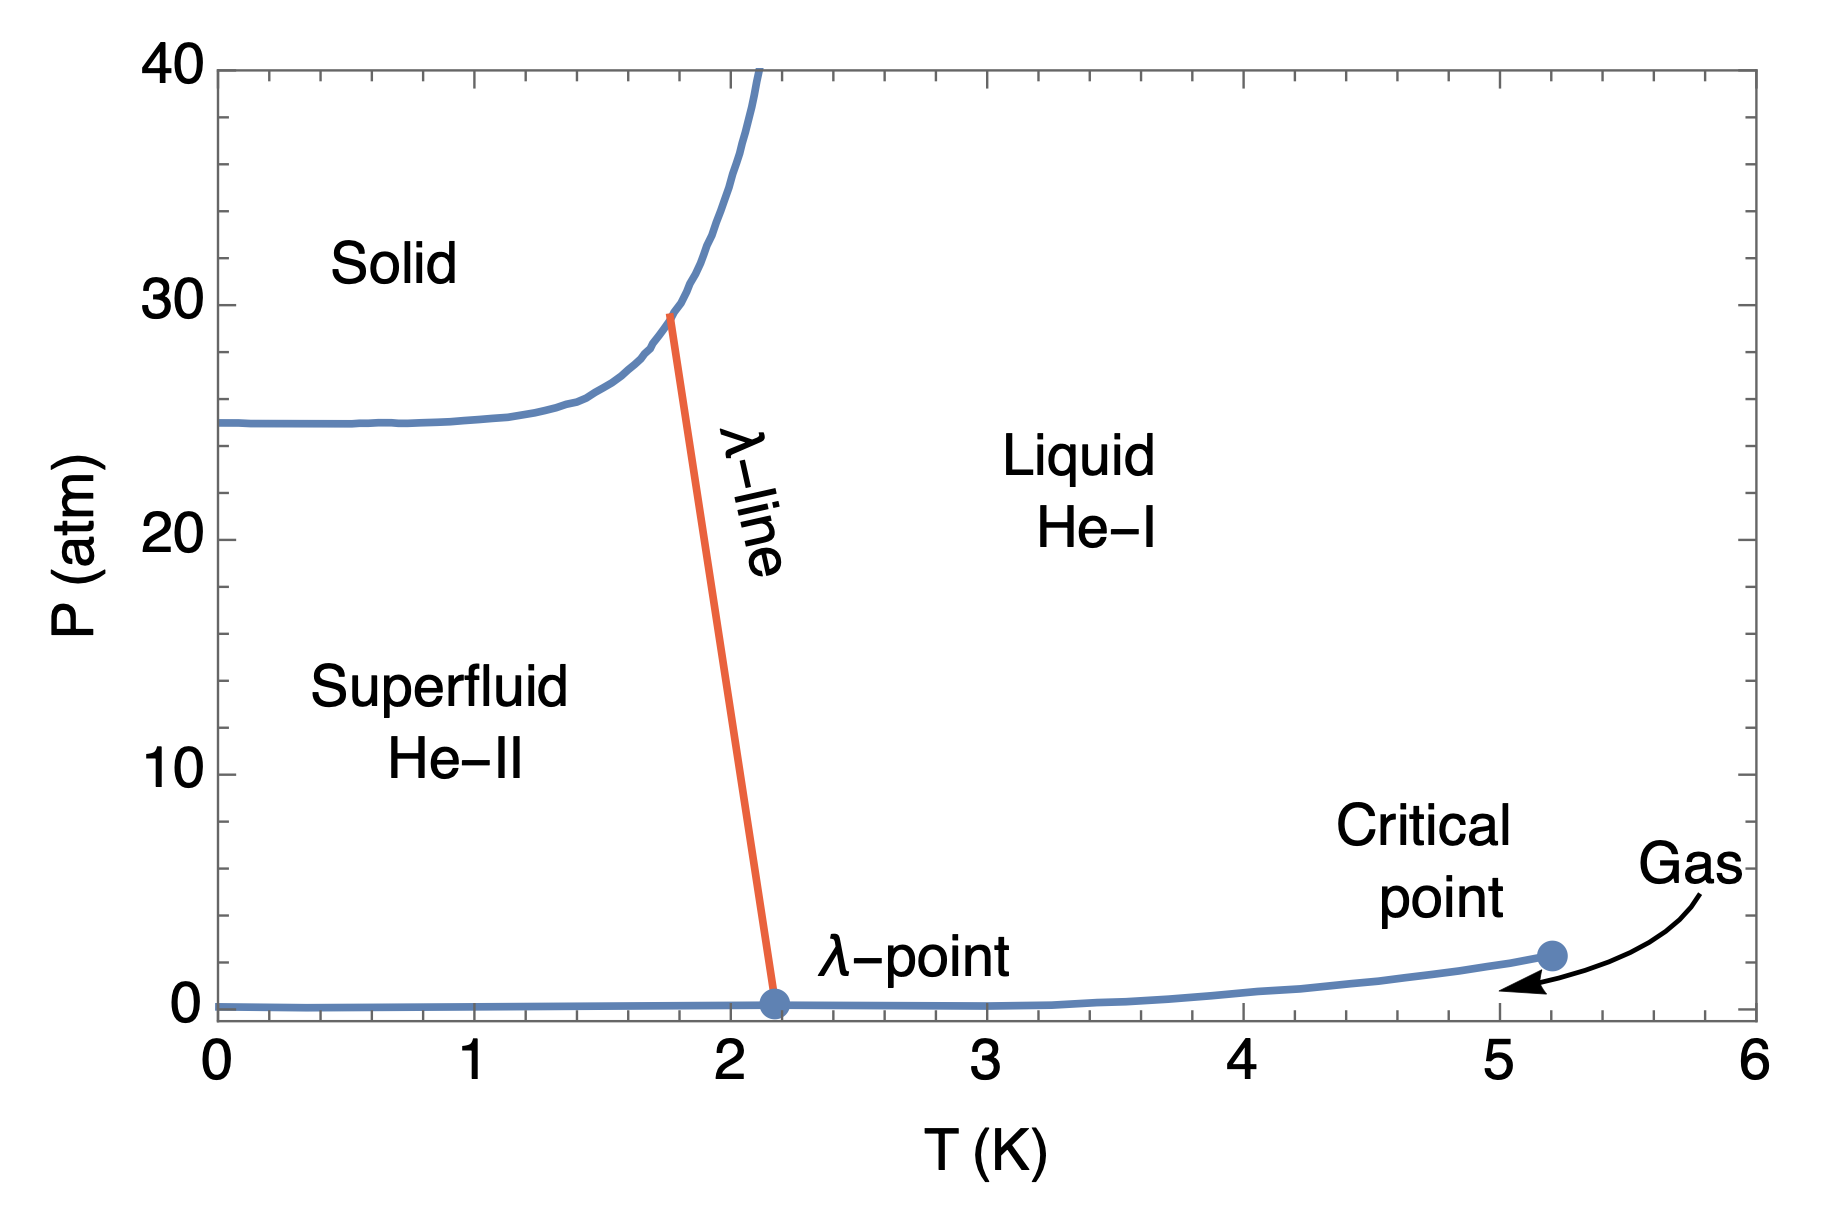
\includegraphics[scale=.3]{lambda_transition.png}
	\caption[Example of  a critical line: $\lambda-$line of  $^4$He]{\label{fig: lambda line}An example of critical line: the phase transition for $^4$He along its whole $\lambda-$line is a continuous phase transition. Figure taken from \cite{Chester:2019ifh}.}
\end{figure}






\subsection{Connecting critical phenomena to conformal field theories}
\subsubsection{A brief review: renormalization group formalism}
\label{sec: review of RG}
In the previous section, we concluded with the universality of the critical phenomena and how the correlation length diverges at the critical point. In this section, we will try to see why this is so and how this relates to conformally invariant theories.

As we stated earlier, the concept of universality can be best understood in the framework of renormalization group flows but I'll assume that the reader may not be familiar with it so I'll briefly summarize the main points of it qualitatively.

Let's remember our phenomenological model for the free energy in \equref{eq: landau potential in path integral}
\be 
e^{-\b F(K_i)}=\int \cD\f e^{-\b L[K_i,\f]}
\ee 
This is a phenomenological model, so the field $\f(x)$ is coarse-grained below a certain length scale, say 1 micrometer. This means we cannot resolve anything below 1 micrometer but do so above it. 

We have seen that the critical phenomena (such as critical opalescence in fluids) happen at a rather macroscopic scale, so let's coarse-grain all the fluctuations of the order parameter $\f(x)$ between 1 micrometer and 1 millimeter. To do so, we separate \emph{all functions} $\f(x)$ as those which only fluctuate above 1 millimeter (call them $\f_l(x)$) and those which fluctuate between 1 millimeter and 1 micrometer (call them $\f_h(x)$).\footnote{Here $l$ and $h$ refer to low and high frequencies respectively. As a side note, it is actually a lot more straightforward to do this separation in Fourier space} As $\int\cD\f$ is a path-integral, it becomes $\int\cD\f_h\int\cD\f_l$,\footnote{For anyone not familiar with the path-integrals, this may seem odd: we divided the whole integration to two parts, so they may expect $\int\cD\f\rightarrow\int\cD\f_h+\int\cD\f_l$. One intuitive (yet not necessarily rigorous) way to see that this isn't the case is to consider the fact that the general function $\f$ has both low and high frequency parts so it is not like $\int_a^bdx=\int_a^0dx+\int_0^bdx$ but rather like $\int dxdy=\int dx\int dy$.} hence we now have
\be 
e^{-\b F(K_i)}=\int \cD\f_l e^{-\b L'[K_i,\f_l]}
\ee 
for 
\be 
e^{-\b L'[K_i,\f_l]}=\int \cD\f_h e^{-\b L[K_i,\f]}
\ee 
If all possible terms allowed by the symmetries of the Hamiltonian are included in the effective potential $L$, then $L'$ should not have any new terms; hence we can write $L'[K_i,\f_l]=L[K_i',\f_l]$, thus we have
\be 
e^{-\b F(K_i)}=\int \cD\f e^{-\b L[K_i,\f]}
=\int \cD\f_l e^{-\b L[K_i',\f_l]}
\ee 
where the first integration is coarse-grained over 1 micrometer and second over 1 millimeter. Of course, there is nothing special about these values and we can generally write
\be 
\label{eq: free energy with Lambda}
e^{-\b F(K_i)}=\int_{\Lambda}\cD\f e^{-\b L[K_i(\Lambda),\f_\Lambda]}
\ee 
where the integration is coarse-grained over distances $\Lambda^{-1}$ and the phenomenological constants in the Landau potential are now functions of the parameter $\Lambda$.

What can we do with this parameter $\Lambda$? On one hand, we can try to take it to infinity (effectively removing any coarse-graining process): this indicates we are trying to probe the microscopic theory and our phenomenological model will eventually break down; indeed, in statistical physics, we cannot take $\Lambda$ bigger than the inverse lattice spacing, i.e. $a^{-1}$. In high energy physics, we do not have a natural microscopic length scale (assuming we are focusing on standard model without gravity) hence we may \naively try to take $\Lambda$ to infinity. In this limit, our theory may or may not fail; it is the experiments that ultimately would invalidate (or not) our models.\footnote{\label{footnote: normalizable vs nonnormalizable}
If our model is so-called \emph{nonnormalizable}, it will surely fail as we keep increasing $\Lambda$; in fact, we may be able to predict beyond which point our model is unreliable. An example of this is Fermi's  four-fermion theory of the weak interaction which breaks down around $\Lambda\sim 300$ GeV. On contrary, if our model is so-called \emph{renormalizable}, then it is self-consistent in the phenomenological sense and hence is insensitive to microscopic theory: we can safely take $\Lambda$ to $\infty$. \emph{However}, the resultant theory is \emph{not necessarily the correct model for the phenomena it is written to describe}. In other words, despite being self-consistent at any scale $\Lambda$, \emph{the predictions} of a renormalizable theory may diverge from the experimental values after a certain $\Lambda$, which indicates a modification of our model is necessary beyond a certain $\Lambda$. The fact that renormalizable theories cannot tell their regime of validity, along with the other fact that nonnormalizable theories necessarily break down beyond an energy scale, leave us with one firm conclusion: \emph{we can never write down a physical theory which is guaranteed to work at all length scales!}
} On the other hand, we can take $\Lambda$ to zero: this means we are \emph{integrating-out} all degrees of freedom, leaving us with the ultimate IR behavior of the theory!\footnote{
As is commonplace in high energy and statistical physics, we will refer the behavior of a a system at very low and very high energies as its IR and UV behavior, where they stand for infrared and ultraviolet (i.e. low and high frequency ligh).
}

The change of $\Lambda$ by \emph{integrating-out} high frequency modes\footnote{Equivalently coarse-graining low distance details.} as we have demonstrated above is called \emph{renormalization group flow}, i.e. RG flow.\footnote{In the full RG flow, we actually also rescale after coarse-graining, and do these infinitesimally so that there is \emph{indeed} a continuous flow of coupling constants under RG.} The main take-away of this argument is that under the change of the \emph{regularization parameter} $\Lambda$, the phenomenological parameters $K_i$ change, i.e. $K_i=K_i(\Lambda)$.

The RG flow as we have briefly introduced above does nothing by itself: it does not compute anything, nor does it give any obvious simplification. In practice, one \emph{combines} a computational technique with RG flow to \emph{improve} that technique; for instance, one can combine RG flow with the perturbation theory to yield \emph{RG improved perturbation}. We do not need to know anything about these in these notes.\footnote{How RG improves perturbation theory is a standard topic, and one can consult their favorite QFT book. In short, instead of having a perturbation expansion with the small parameter $g\log\left(\frac{p^2}{m^2}\right)$, we do a perturbation expansion with the small parameter $g_\mu$ which is computed by RG flow of the parameter $g$. The second expansion is improved because $\log$ terms can get large for large momenta $p^2$.
} For our purposes, all that matters is that the phenomenological constants $K_i$ in our Landau model changes with the regularization scale $\Lambda$. 

Let's try to extend this formalism from statistical mechanics to high energy theory: in a $d-$dimensional Euclidean QFT,\footnote{The argument is same for Lorentzian QFTs as well.} the vacuum generating function $Z$ is given as\footnote{See footnote~\ref{footnote: vaccum generating function} for a reminder on the vacuum generating function Z.} 
\be 
Z[K_i]=\int \cD \f e^{-\int d^dx\cL[K_i,\f(x)]}
\ee 
where $\f(x)$ collectively denotes all fields, and $K_i$ are usually called \emph{coupling constants}.\footnote{In general, the Lagrangian\footnotemark has the form
\be 
\label{eq: most general form of Lagrangian}
\cL[K_i,\f(x)]=\sum_i K_i\cO_i(x)
\ee 
where $\cO_i(x)$ are \emph{operators} in the theory and $K_i$ are coupling constants, i.e. terms that couple the operators to the Laplacian. The operators can be of various forms, simple examples are $\cO_1(x)=\f(x)$ and $\cO_2(x)=\f(x)^2$. If the theory is free or we are perturbing around a free theory, such operators are not really independent (I can imagine some readers already shouting \emph{``one is the square of the other!''}). However, if the theory is strongly coupled, it may not be possible to write down $\cO_i(x)$ simply as $\f(x)$ or $\f(x)^2$; the very same operators that were $\f(x)$ and $\f(x)^2$ in the weak coupling regime can get radically different in the strong coupling regime: we will see an example of that in \emph{the 3d Ising model} below.
}\footnotetext{In these notes we are abusing the language and refer both to the Lagrangian and the Lagrangian density as Lagrangian for short, which is a fairly common practice in the field.} We do not have a natural regularization parameter here as we did in the Landau theory (or inverse lattice spacing $a^{-1}$ as in statistical mechanics), so the integration is \naively over all length scales. However, this is too ambitious: as we stated in footnote~\ref{footnote: normalizable vs nonnormalizable}, we can actually never write down a theory which is \emph{guaranteed} to work at all length scales (according to our current understanding). Thus we have two choices: if our Lagrangian is \emph{nonnormalizable}, we already need a momentum cut-off $\Lambda$ because our model is guaranteed to fail above a certain threshold. If our Lagrangian is \emph{renormalizable}, then in principle we do not need a cut-off for consistency,\footnote{There are infinities if we don't regularize our integral, but in a normalizable theory these infinities can be removed. So, in effect, even if we put a cut-off $\Lambda$, we can consistently take $\Lambda\rightarrow\infty$; but we do not need to put a cut-off in the first place (we can regularize the infinities in other ways, such as dimensional regularization).} though the model may still break down (i.e. cannot explain experiments) after a certain energy threshold $\Lambda$. In short, for both cases, it is logical to keep an arbitrary regularization scale $\Lambda$ in the integration, reminding us that we are not integrating over modes  with higher frequency than arbitrary $\Lambda$:
\be 
Z[K_i]=\int_\Lambda \cD \f e^{-\int d^dx\cL[K_i(\Lambda),\f_\Lambda(x)]}
\ee 
Such theories are called \emph{effective field theories}, and we just argued that all quantum field theories are in a sense effective field theories!\footnote{\label{footnote: decoupling principle}
A related concept here is \emph{the decoupling principle}. It basically states that if we have a very heavy particle in our model, its existence in low energies is only reflected through the modification of the coupling constants of lighter particles. In other words, in low energies, the heavy particles \emph{decouple} from the effective description of the phenomena (in the jargon, their propagators are said to be \emph{frozen}, or that they can be\emph{ integrated out}). As a corollary of the decoupling principle, we can never know certainly if there are heavier particles which have not been yet discovered by doing experiments at low energies; because if there are such particles, their contribution to the observables are indistinguishable from their absence with a different set of coupling constants of lighter particles.
}

Let's get back to our main take-away both in statistical mechanics and high energy physics: the coupling constants in the Lagrangian (or Hamiltonian in statistical mechanics) change as we change the regularization scale $\Lambda$. But what exactly does that mean?

To understand the situation better, let us consider a single scalar field $\f(x)$ in three space dimensions with the Lagrangian:
\be 
\label{eq: 3d scalar field}
\cL=\half(\partial\f)^2-\frac{m^2}{2}\f(x)^2-\frac{\lambda}{4!}\f(x)^4-h\f(x)
\ee 
We are describing a \emph{massive} scalar field which self-interacts with the interaction strength $\lambda$. We observe three things:
\begin{enumerate}
	\item We could have written $h(x)$ instead of $h$ and treat the magnetic field $h(x)$ as a classical background field (i.e. it does not have a kinetic term).\footnote{From QFT point of view, that makes much more sense as we can use $h(x)$ as a source term to take functional derivatives of the vacuum generating function $Z$ to construct correlation functions. Our main point here is not that so we are simplifying the situation for a clearer discussion.} Rather, $h$ is simply a coupling constant in this setting, such as $m^2$ and $\lambda$.
	\item The Lagrangian has $\Z_2$ symmetry (same symmetry with Ising Universality Class) if $h=0$, i.e. it is invariant under $\f(x)\rightarrow-\f(x)$.
	\item We could add other terms consistent with the $\Z_2$ symmetry to the Lagrangian, i.e. $\f(x)^6$. The absence of such terms are yet not warranted but we'll argue later that it is a consistent and reasonable omission.
\end{enumerate}
Let us now apply an RG transformation: as we discussed above, this will change the coupling constants (in this case $m^2$, $\lambda$, and $h$) as we iterate the RG flow. If we start with \emph{small} $m^2,\lambda,$ and $h$ for $d>4$,\footnote{In these notes, $d$ always denotes the dimensionality of the space unless stated otherwise.} we can show that $\lambda$ gets smaller with RG: we call such coupling constants \emph{irrelevant}.\footnote{\label{footnote: relevant vs irrelevant}More correctly, we call a coupling constant (or the direction it forms on the phase diagram) \emph{irrelevant for the point} $p$ if RG flow takes the coupling constant \emph{towards} $p$. For instance, for the point $\lambda=0$, the coupling constant $\lambda$ is irrelevant because RG takes $\lambda$ closer and closer to $0$. On the contrary, if the RG transformation takes the value \emph{away} from point $p$, then that direction is said to be \emph{relevant for the point }$p$. For instance, for the point $h=0$, the coupling constant $h$ is relevant because RG takes any nonzero $h$ further and further away from $0$. If RG moves a variable $x$ neither towards to nor away from a point $p$, then $x$ is said to be \emph{a marginal direction} for point $p$.

For the concept of being relevant and irrelevant to be mutually exclusive for a point $p$, the RG transform should not \emph{reach} to that point in finitely many iterations; otherwise, it can move towards the point $p$ in the first $n$ iterations and move away from it in the remaining iterations, making the direction both irrelevant and relevant! Thus, the points $p$ that we referred above should be \emph{fixed-points}: points that RG transformation reaches in \emph{infinitely} many iterations. Also, if we are \emph{exactly at} those fixed points, then we stay at them under RG, i.e. they are \emph{invariant points of RG flow}!


In summary, relevant and irrelevant directions are respectively the unstable and stable directions of the fixed point under perturbation.
} On the other hand, $m^2$ and $h$ are relevant coupling constants, i.e. they get larger under iterations of RG flow.\footnote{See footnote~\ref{footnote: relevant vs irrelevant}.} In the coordinate system where the coupling constants are axes, which is actually precisely the phase diagram we have been analyzing in the previous sections, relevant coupling constants form the directions that need to be tuned to reach the critical point; for instance, for $d>4$, $(h,m^2,\lambda)=(0,0,0)$ describes the critical Ising model ($m^2$ plays the role of the critical temperature, much like $a$ did in \equref{eq: Landau potential} for the Landau description of the Ising model)
and we need to tune $h$ and $m^2$ to reach this point ($\lambda\rightarrow 0$ by itself under RG). On the other hand, if $d<4$, things get a little bit complicated: $\lambda$ is also relevant now hence $(h,m^2,\lambda)=(0,0,0)$ no longer describes the Ising universality class: it now has 3 relevant directions hence 3 parameters need to be tuned (unlike the fluids or uniaxial magnet).\footnote{Remember that we should tune temperature $T$ and external magnetization $h$ for magnets and temperature $T$ and pressure $p$ for fluids.} However, if $d$ is \emph{very close to 4} (say $d=3.99$), then $\lambda$ is barely relevant and we can expect a new critical point close to $(0,0,0)$, which corresponds to Ising Universality class.\footnote{One motivation for this is called \emph{cross-over} phenomena. Basically it says that despite $\lambda$ is relevant, we still spend a lot of time around the critical point during RG (as $\lambda$ is barely relevant), hence we can effectively treat $\lambda$ as an irrelevant parameter. The end of section 5.4 of \cite{Cardy:1996xt} touches on this, in fact simply see the whole chapter for a thorough discussion.} In fact, in their 1971 paper titled \emph{Critical exponents in 3.99 dimensions} \cite{Wilson:1971dc}, Wilson and Fisher found such a point and computed the critical exponents as expansion of the small parameter $\e=4-d$. One can reach this critical point (1) by tuning $m^2/\lambda$\footnote{The precise value of this ratio to reach the critical point is not unique and depends on the chosen UV regularization of the theory \cite{Simmons-Duffin:2016gjk}.} so that one is on the \emph{critical surface} and then (2) by applying the RG flow which will take the system away from the Gaussian point and towards this new point: see \figref{\ref{fig: Wilson-fisher}} for the diagrammatic illustration of this procedure along with the RG flows on the phase diagram of the $3d$ scalar.

\begin{figure}
	\centering 
	$(a)\begin{aligned}
		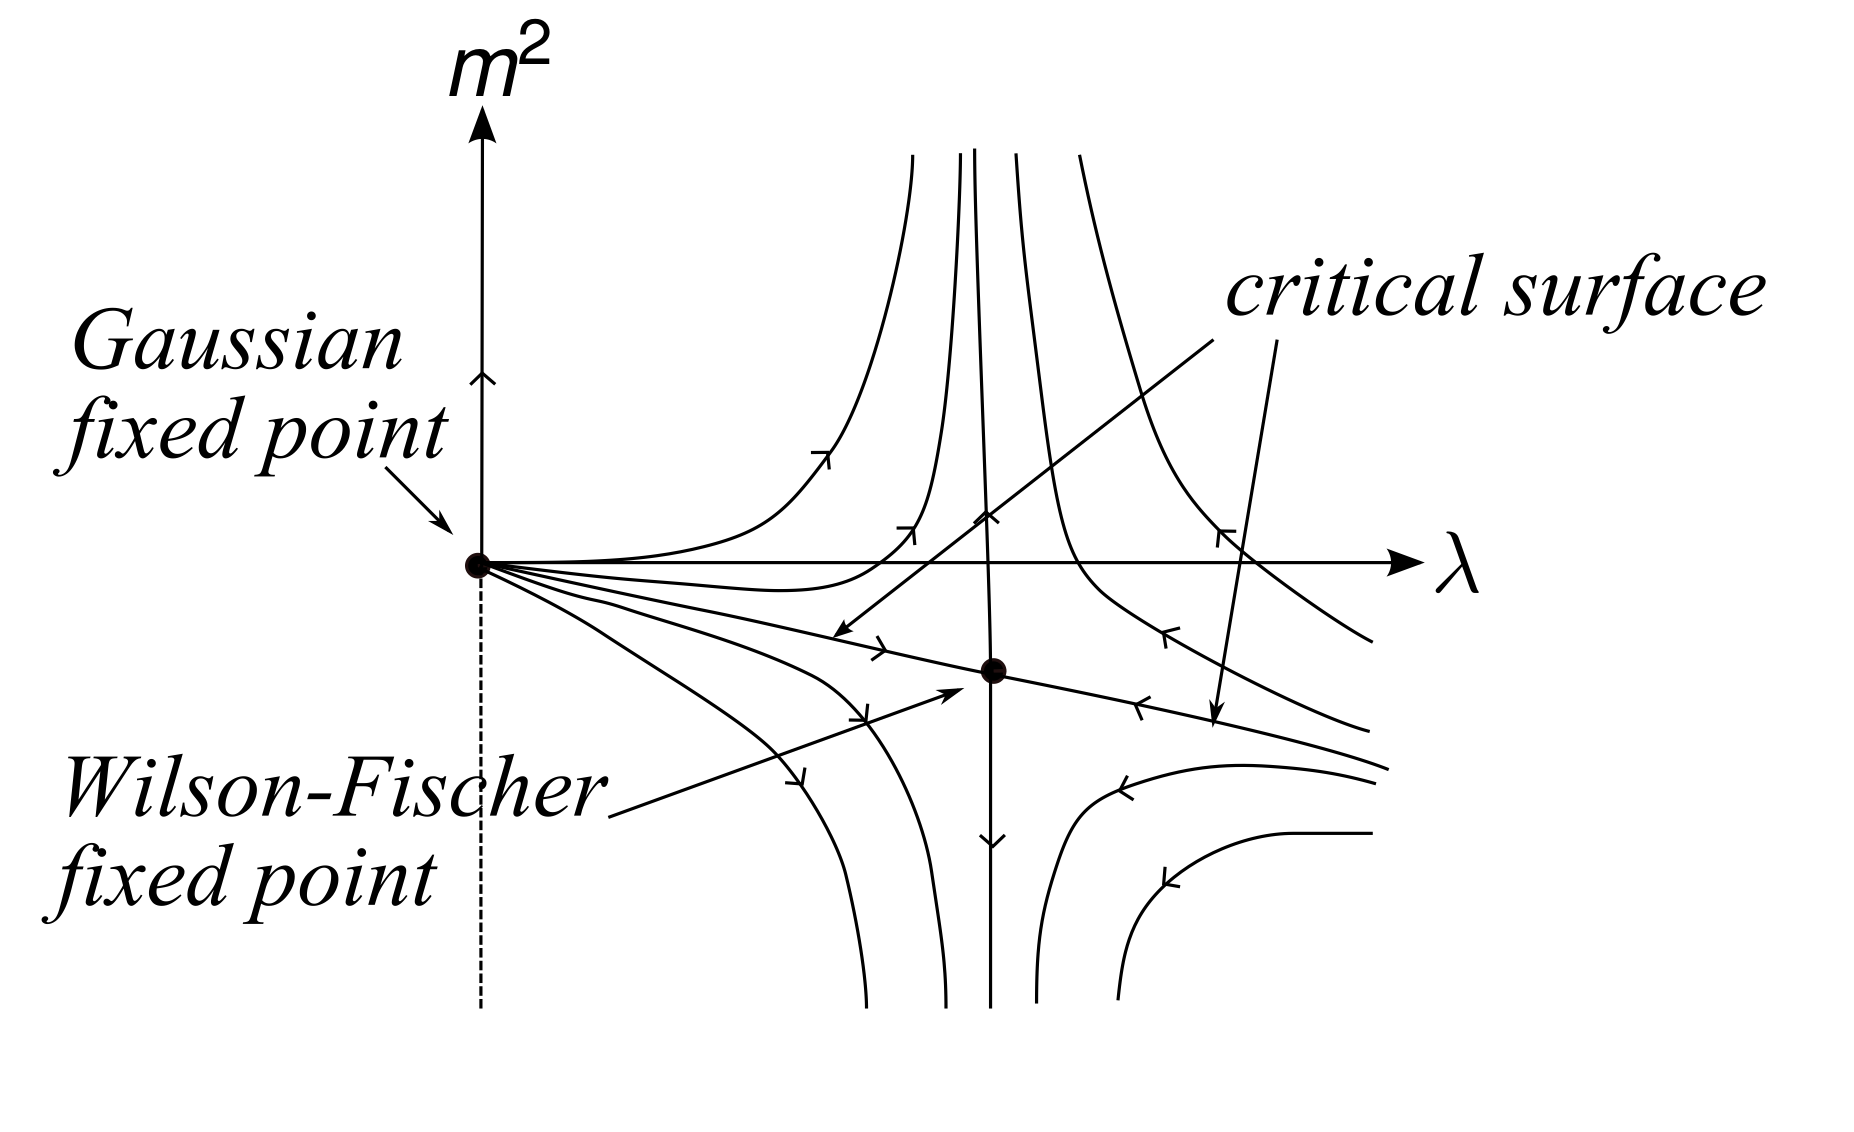
\includegraphics[scale=.26]{RG_flow_for_Scalar.png}
	\end{aligned}\quad 
	(b)\;\;
	\begin{aligned}
		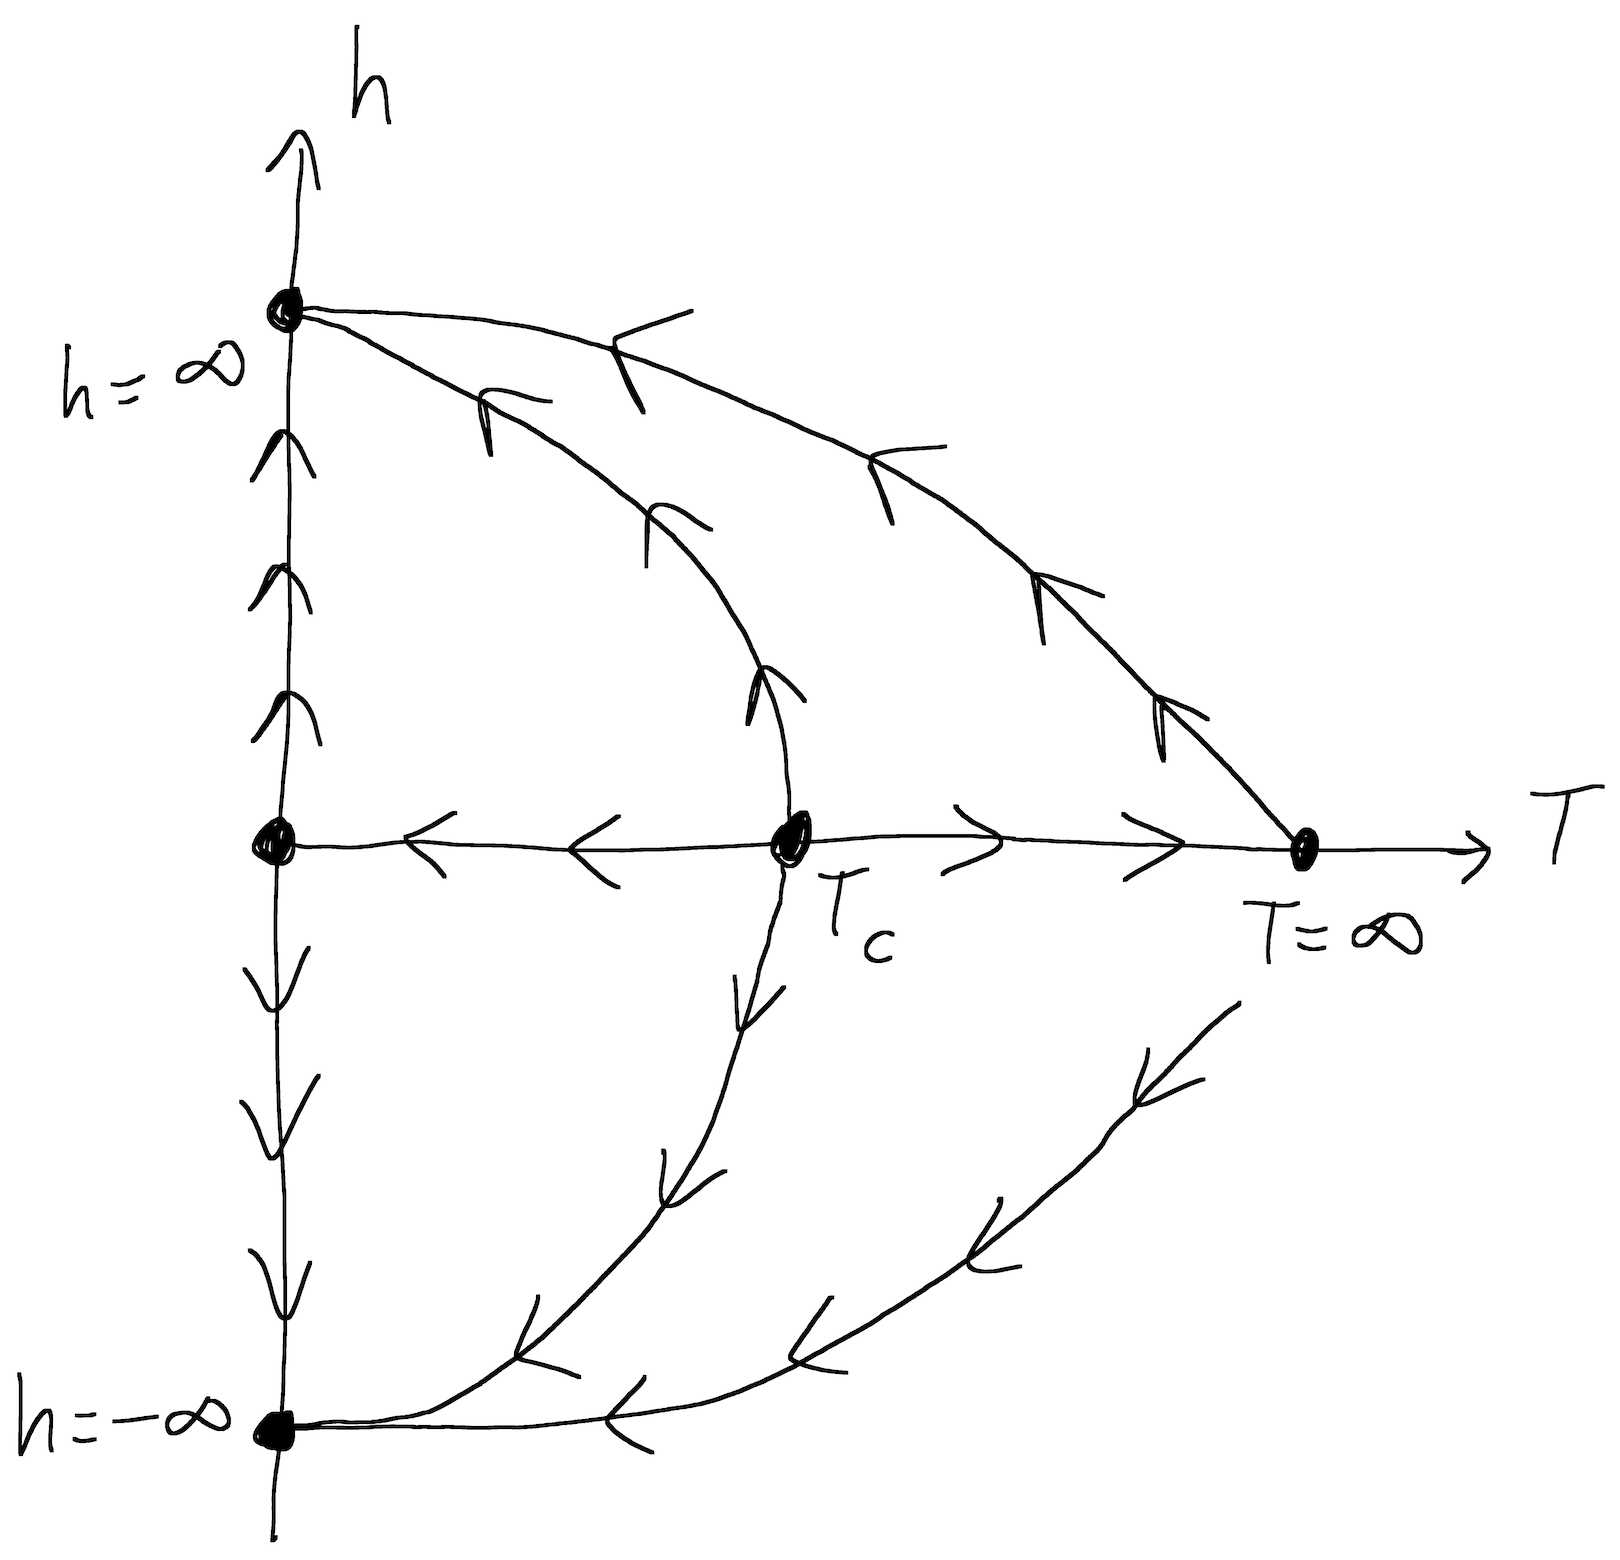
\includegraphics[scale=.2]{RG_flow_for_Magnet.png}
	\end{aligned}$	
	\caption[RG flows for the $3d$ scalar field and the uniaxial magnet]{\label{fig: Wilson-fisher}\textbf{(a)} Phase diagram of the $3d$ scalar field with $\Z_2$ symmetry, with the RG trajectories shown. We see that the coupling constants move towards four possible fixed points under RG transformation: two sinks at $m^2=\pm\infty$, one Gaussian fixed point, and one interacting fixed point called \emph{Wilson-Fischer fixed point}. \textbf{(b)} Phase diagram for uniaxial magnet , with the RG trajectories shown (see also \figref{\ref{fig: phase diagram}}). There are five fixed points: one Gaussian fixed point at $h=T=0$, two sinks at $h=\pm\infty$, one interacting fixed point at $\{T,h\}=\{T_c,0\}$, and one non-interacting fixed point at $T=\infty$.}
\end{figure}

Thus, in summary, the description of a system (the values of coupling constants) change by at which scale we look at the system (different regularization $\Lambda$), and the modification in the description of the system as we change our perspective can be shown as a flow in the phase diagram for the system: this is called \emph{RG flow} and \figref{\ref{fig: Wilson-fisher}} illustrate this for a scalar field and uniaxial magnet.

Let's comment more on \figref{\ref{fig: Wilson-fisher}a}. We observe that there are four fixed points for the RG flow; \emph{the Gaussian fixed point}, i.e. $\lambda=h=m^2=0$,\footnote{It is called so because the Lagrangian is then Gaussian.} two sinks\footnote{These fixed points are called sinks because they do not have any relevant direction: a system never moves away from sink under RG flow!} at $m^2=\pm\infty$, and \emph{the Wilson-Fisher fixed point} at $(m^2,\lambda)=(m^2_c,\lambda_c)$. In comparison, \figref{\ref{fig: Wilson-fisher}b} has five fixed points: one Gaussian, two sinks, one critical fixed point (at Curie temperature), and one so-called discontinuity fixed point at $T=\infty$. We review types of different fixed points in \tabref{\ref{table:classification of fixed points}} at the end of this section.

Let's take a step back and review our situation: we stated above that the $3d$ scalar theory at Wilson-Fisher fixed point is in $3d$ Ising Universality Class, but what exactly is the Lagrangian for this theory? Can we compute the critical exponents analytically and exactly? Even before all these, what exactly do we know about this point?

Our questions are rather valid and to the point (pun intended), but the answers will be disappointing. We remind the reader that we started \emph{around} the Gaussian fixed point $m^2=\lambda=h=0$, and said that Wilson and Fisher found a new fixed point nearby. This procedure is in fact no coincidence: we have no way to map out the RG flow exactly and completely, and we have no way of doing actual computations (like literal computation of the path integrals and such) unless we are nearby the Gaussian fixed point. Thus, necessarily, we start around the Gaussian fixed point and look for new fixed points as Wilson and Fisher did.

The previous paragraph is rather disturbing: it basically means we somehow stumbled upon the Wilson-Fisher fixed point, and maybe there are a lot more fixed points that are unbeknownst to us! Indeed, by the conventional way of doing things (which I'll list below), there is no way we can guarantee that we do not have new fixed points, and hence there is no guarantee that Wilson-Fisher fixed point is the correct one to describe the $3d$ Ising Universality Class. The more modern\footnote{This adjective may be unfair to other methods, but with my limited knowledge this is how I see it.} way of mapping the fixed points of a phase diagram is in fact to \emph{look for} conformal field theories with correct number of relevant operators and the correct symmetry group (more on this below). For instance, it is shown in \cite{Kos:2014bka} by conformal bootstrap techniques that \emph{``...3D Ising CFT is the only $\Z_2-$symmetric CFT in 3 dimensions with exactly two relevant operators...''}, which indicates that if the Wilson-Fisher fixes point is describing the $3d$ Ising CFT, then there can be no other fixed points with two relevant operators which describe a $\Z_2-$symmetric CFT in the whole phase diagram!\footnote{There is a always a chance that there is a fixed point with scale symmetry without conformal symmetry, but this is quite unlikely: we'll elaborate on this later.}

Before detailing this conformal bootstrap approach, we need to fully appreciate why this approach is powerful \emph{and necessary} in the first place! To do so, let's give some general remarks and comment on a few points:
\begin{itemize}
\label{items: problems with strongly coupled systems}
	\item Strongly coupled quantum field theories (or statistical models) are not soluble!\footnote{Of course, this is a generic statement and there are exceptions. However, to my knowledge, they are either in low dimensions (such as 1d or 2d models) or have additional symmetries (such as supersymmetry of conformal symmetry). \draftnote{Put references here}} Not only do we not have the required mathematical tools to solve them, but also do we not have the mathematical framework to \emph{hope} to solve them in future!\footnote{We are talking about the impossibility of finding an algorithm to solve them \emph{generically} because of the undecidable nature of the mathematical problem (see footnote~\ref{footnote: decidability}).}
	
	
	\item If we cannot analytically solve the problem, we can try numerically solving it on a computer! For that, we put the theory on a lattice (we need a discretization to employ the computer) and simulate its behavior. The branch of the physics that adopts this approach is called \emph{lattice simulations}.\footnote{\draftnote{Add some sources here}} Despite its relative success, this approach is limited because (a) the computing power is limited and (b) the complexity of the problem can be rather high to utilize this approach!\footnote{For instance, the problem of solving $3d$ Ising model on the lattice is shown to be an \emph{NP-complete problem} in 2000 \cite{istrail2000statistical}; basically meaning that it is not feasible in practice to try to solve this model on a lattice!}
	
	\item We can solve free theories.\footnote{Gaussian path-integrals are the only path-integrals we can compute exactly. \draftnote{This is certainly true in standard statistical mechanics and QFT context but I wonder if there are exotic functions which can be analytically computed as well, maybe I can look into that!}} As we cannot solve strongly coupled theories, we can assume weak-coupling and do perturbation theory: this is basically what we do for most of the standard model!\footnote{We are rather lucky that the couplings of the electroweak theory (describing, electric, magnetic, and weak interactions) are rather small at the typical energies we observe the universe, so that we can use perturbation theory to describe the world successfully! }
	
	\item If we cannot take the coupling constants to be small, we can try to vary other parameters and try to find a free theory this way. For instance, instead of considering a scalar field $\f(x)$, we can consider $N$ copies of it: most of the time the theory is free if $N\rightarrow\infty$; we can then (1) do an expansion around that free theory, (2) compute corrections order by order in $1/N$, (3) assume that truncation at some order is fine, (4) take $N=1$ (or whatever the original number of copies) at the end. This procedure is called \emph{large N expansion}, see \cite{Moshe:2003xn} for a 200-page review of this concept!
	
	\item Another parameter that we can vary to approach a free theory is the dimension of the space itself! As we noted above, there exists a fixed point (Wilson-Fisher fixed point) if $d<4$ and this fixed point merges with the Gaussian fixed point as $d$ approaches $4$. As we know how to deal with the Gaussian fixed point, we can take $\e=d-4$ to be small so that the Wilson-Fisher fixed point is close enough for us to use our Gaussian fixed point knowledge to analyze that critical point (and this is how that critical point was discovered in the first place)! This approach is called \emph{epsilon expansion}, and in a sense similar to large N expansion: we expand in $\e$, compute first few terms, truncate the expansion, and take $\e\rightarrow1$ to get the critical point of $3d$ Ising model.\footnote{There is a whole bunch of literature on the validity of this approach and how to improve it. \draftnote{Add references}}
\end{itemize}

The items above show how desperate our situation actually is as theoretical physicists! Nevertheless, do not despair! We can still make progress in the realm of strongly coupled theories by realizing that fixed points are actually scale-invariant, hence they enjoy a higher symmetry than the rest of the phase diagram!

Let me expand on the scale invariance. Under RG transformation, the correlation length $\xi$ scales linearly, i.e. it behaves as $\xi\rightarrow l \xi$. Thus, at the fixed points of the RG transformation, $\xi$ is either $0$ or $\infty$. As a corollary, \emph{any point at the phase diagram where the correlation length diverges is a fixed point of the RG flow!} Hence, by our discussion in the previous section we can conclude that the critical phenomena happen at some of the fixed points of the RG flow! \emph{ In short, understanding the nature of fixed points and the emergent scale invariance is invaluable to understanding critical phenomena!}


Let us end our scandalously lightening review of  RG flow and turn to the relation to the conformal field theories in the next section; but before that, we present \tabref{\ref{table:classification of fixed points}} as a general reference: it contains a brief categorization of fixed points according to their dimensionality and the value of correlation length, see Table~9.1 of \cite{Goldenfeld:1992qy} for the original/better version of it.

\begin{table}
	\scriptsize
	\caption{\label{table:classification of fixed points}Classification of fixed points}
	\centering
	\begin{tabular}{lllll}
		\hline\hline
		\textbf{\# of relevant directions} & \textbf{$\xi$}&\textbf{Type of fixed point}&\textbf{Physical Domain}&\textbf{Explanation}\\\hline
		0&0&Sink&Bulk phase&\begin{minipage}{.4\textwidth}
			No relevant directions, hence trajectories only flow to them: they correspond to \emph{stable bulk phases}, and the nature of the coupling constant characterize the phase; e.g., in $3d$ Ising model with nearest neighbor ferromagnet interaction in external field $h$, there are two sinks at \mbox{$h=\pm\infty$\&$T=0$}, indicating the stable bulk phase is a net magnetization in all temperatures, whose sign is determined by sign of $h$.
		\end{minipage}
		\\\hline
		1&0&Discontinuity FP&Plane of coexistence&
		\begin{minipage}{.4\textwidth}
			Correspond to points on a phase boundary and describe \emph{a first order phase transition} where an order parameters exhibits discontinuous behavior (\emph{We note that the interpretation of RG transformations near first order phase transformations is delicate }and this explanation is rather simplified, see \cite{Sokal:1991ui} for a careful discussion). E.g., all points on the line \mbox{$h=0, T<T_c$} in a ferromagnet flow to a discontinuity FP at \mbox{$h=0,T=0$}. This FP is unstable towards the sinks. Lastly, this is the only fixed point where one of the eigenvalues of the real space RG flow is $l^d$.\footnotemark
		\end{minipage}
		\\\hline 
		1&0&Continuity FP&Bulk phase&
		\begin{minipage}{.4\textwidth}
			Represents \emph{a phase of the system}, e.g. \mbox{$h=0, T=\infty$} which attracts all points on the line \mbox{$h=0,T>T_c$} in a ferromagnet. Phases described by this FP are unstable towards a sink.
		\end{minipage}
		\\\hline 
		2&0&Triple point&Triple point& Nothing interesting.
		\\\hline
		2&$\infty$&Critical FP&Critical manifold& \begin{minipage}{.4\textwidth}We explained this whole section.\end{minipage}
		\\\hline
		Greater than 2&$\infty$&Multicritical point&Multicritical point&\begin{minipage}{.4\textwidth} Higher-dimensional generalization of what we have explained this whole section.\end{minipage}
		\\\hline
		Greater than 2&0&Multiple coexistence FP&Multiple coexistence& Nothing interesting.
		\\\hline\hline
	\end{tabular}
\end{table}
\footnotetext{Let $l$ be a coarse-graining factor and $d$ is the dimension of the system. If one of the eigenvalues of the RG flow near a critical point is $l^d$, then that critical point is either a first-order or a discontinuity fixed point! All other fixed points have $y<d$ for the eigenvalue $l^y$, see Table~\ref{table:classification of fixed points}. This is called \emph{Nienhuis-Nauenberg criterion}, see \cite{Nienhuis:1975zs} for further details.}


\subsubsection{Dimensional counting  and scale invariance}

Let us consider the most generic form of the Lagrangian we gave in \equref{eq: most general form of Lagrangian}, i.e. $\cL[K_i(\Lambda),\f(\Lambda,x)]=\sum_i K_i(\Lambda)\cO_i(\Lambda,x)$. The action then reads
\be 
S=\sum_i\int_\Lambda d^dx K_i(\Lambda) \cO_i(\Lambda,x)
\ee 
where $\Lambda$ is \emph{the momentum cut-off}, i.e. the regularization parameter.\footnote{As we stated earlier, we need this parameter in statistical mechanics and in nonnormalizable quantum field theories. For renormalizable qft models, we can take it to infinity self-consistently but let's keep it for the sake of argument.} If we scale $x\rightarrow l^{-1}x$, then the lower limit $\Lambda^{-1}$ gets scaled as well, hence we get
\be 
\int_\Lambda d^dx K_i(\Lambda) \cO_i(x)=\int_{l^{-1}\Lambda} d^d(l^{-1} x) K_i(\Lambda) \cO_i(\Lambda,l^{-1} x)
\ee 
If we further scale $\Lambda\rightarrow l \Lambda$, we then obtain the relation
\be 
K_i(\Lambda) \cO_i(\Lambda,x)=l^{-d}K_i(l\Lambda)O_i(l\Lambda,l^{-1} x)
\ee 

In general, the coupling constants' functional form can be rather complicated; after all, this is what determines the flows in \figref{\ref{fig: Wilson-fisher}}. However, near critical point, we can \emph{linearize} the action of RG flow to leading order, hence the coupling constants takes a homogeneous form:\footnote{We call a function homogeneous in its $n^{\text{th}}$ argument if it satisfies $f(\dots,a x_n,\dots)=a^kf(\dots,x_n,\dots)$.}
\be 
\label{eq: scaling of coupling constant}
K_i(l \Lambda)=l^{[K_i]}K_i(\Lambda)
\ee 
where $[K_i]$ is called the \emph{mass dimension} of $K_i$.\footnote{Actually, we are glossing over an important detail here. When we linearize RG flow, it takes the form of a matrix equation, i.e. 
	\be 
	\begin{pmatrix}
		K_1\\K_2\\\vdots
	\end{pmatrix}'
=M	\begin{pmatrix}
	K_1\\K_2\\\vdots
\end{pmatrix}
	\ee 
The coupling constants themselves do not simply scale as in \equref{eq: scaling of coupling constant} individually, but rather their combinations as eigenvectors of $M$ does so. In fact eigenvalues of $M$ determines how they'll scale as well, i.e. their mass-dimensions! However, as this detail is not really necessary for the main discussion, I'll assume in the text that $M$ is diagonal hence $K_i$ can satisfy \equref{eq: scaling of coupling constant}.
} This then indicates $ \cO_i(\Lambda,x)=l^{[K_i]-d}O_i(l\Lambda,l^{-1} x)$.
This equation suggests that $\cO_i$ also transforms homogeneously if we write it in terms of right variables. Instead of writing it as $\cO(\Lambda,x)$, let us write it as $\cO(\Lambda,\Lambda x)$ for the energy scale $\Lambda$ and the dimensionless parameter $\Lambda x$. Thus
\be 
\label{eq: mass dimension of an operator}
\cO_i(l\Lambda,\Lambda x)=l^{d-[K_i]}\cO_i(\Lambda,\Lambda x)
\ee 
Clearly $\cO_i(\Lambda,\Lambda x)$ is a homogeneous function in its first variable: $\cO_i(l\Lambda,\Lambda x)=l^{[\cO_i]}\cO_i(\Lambda,\Lambda x)$ for the \emph{mass dimension} of the operator $\cO_i$. We then conclude
\be 
\label{eq: relation of mass dimensions}
[K_i]+[\cO_i]=d
\ee 

In footnote~\ref{footnote: relevant vs irrelevant}, we categorized coupling constants by their relevance around the critical point, i.e. whether they need to be tuned or not. There, we said that an irrelevant coupling constant vanishes by RG flow aroung the Gaussian fixed point. We see from \equref{eq: scaling of coupling constant} and \equref{eq: relation of mass dimensions} that we can determine the relevance of coupling constants by the scaling dimension of the operator that accompanies them:
\be 
\cO\text{ is called }\left\{\begin{aligned}
\text{ a relevant}\\
\text{ an irrelevant}\\
\text{ a marginal}
\end{aligned}\right\}\text{ operator if}\left\{\begin{aligned}
[\cO_i]<d\\
[\cO_i]>d\\
[\cO_i]=d
\end{aligned}\right\}.
\ee 
Therefore, we can ignore all irrelevant operators $\cO$ in the Lagrangian if we are interested in studying the critical behavior, because their contribution goes to zero as we near the critical point. This is precisely why we truncated higher order terms, i.e. $\f^6$, in \equref{eq: 3d scalar field}.\footnote{There is an important detail that we are glossing over: \emph{dangerously irrelevant operators}. Some operators cannot be just dropped even though their contribution vanishes as we approach the critical point. This is simply because the partition function $Z$ (or vaccum generating function in high energy physics) may not be analytic in that limit. To understand this, let's consider $Z=Z[K_r,K_i,K_d]$ for relevant $K_r$, irrelevant $K_i$, and dangerously irrelevant $K_d$ coupling constants. Under RG, $K_r$ gets bigger so we keep it there. On the contrary, $K_i\rightarrow 0$, hence we can replace it with $0$: $Z=Z[K_r,0,K_d]$. Similarly, $K_d$ goes to zero as well, but we cannot replace it because the function $Z$ is \emph{not analytic} around $K_d=0$. Instead, it behaves like this: \be 
\lim\limits_{K_d\rightarrow0}Z[K_r,0,K_d]=\lim\limits_{K_d\rightarrow0} \frac{1}{K_d^\a}Z'[K_r]
\ee 
for some parameter $a>0$. In short, an irrelevant coupling constant is called \emph{dangerously irrelevant} if the partition function is singular as that term vanishes.

This detail is not really important for our current discussion so we will omit any subtlety related to this.
}

Around the Gaussian fixed point (i.e. the free theory), we can write down operators in terms of the fundamental field in the Lagrangian; for instance, we can take\footnote{In QFT, we should actually define our operators after normal ordering, i.e. \mbox{$\cO_2(x)=:\f(x)\f(x):$}, \mbox{$\cO_3=:\f(x)\f(x)\f(x):$}, etc. This is to ensure that we can put multiple operators at the same spacetime point without any divergence (by normal ordering, we are actually removing the divergence). For instance, the correlator \mbox{$\<\f(x)\f(x)\>=\infty$} whereas \mbox{$\<:\f(x)\f(x):\>=0$}. This detail is not important for the main discussion in the text.}
\be 
\cO_1=\f\;,\quad \cO_2=\f^2\;,\quad \cO_3=\f^4\;,\quad
\cO_4=\f^{6}\;,\quad \cO_5=T_{\mu\nu}=g_{\mu\nu}\cL+\partial_\mu\f\partial_\nu\f
\ee 
where $T_{\mu\nu}$ is the stress tensor of the theory and $\cL$ refers to the Lagrangian in \equref{eq: 3d scalar field}.\footnote{The computation of the stress tensor is most conveniently done by changing the Euclidean/Lorentzian metric to an arbitrary one $g_{\mu\nu}$ and then variate the Lagrangian with respect to it, i.e. $T^{\mu\nu}\equiv\frac{2}{\sqrt{g}}\frac{\delta\left(\sqrt{g}\cL\right)}{\delta g_{\mu\nu}}$ for $g=\abs{\det(g_{\mu\nu})}$.} As the Lagrangian includes a term $(\partial\f)^2$ without a coupling constant in the front,\footnote{This is how we normalized our field $\f$ in the first place, which is rather conventional.} \equref{eq: relation of mass dimensions} indicates $[\partial\f]=d/2$, hence $[\f]=\frac{d-2}{2}$, thus this gives us
\be 
\label{eq: mass dimensions aroung Gaussian fixed point}
[\cO_1]=\frac{d-2}{2}\;,\quad [\cO_2]=d-2\;,\quad [\cO_3]=2d-4\;,\quad [\cO_4]=3d-6\;,\quad [\cO_5]=d
\ee 
We see that $\cO_1$ and $\cO_2$ are always relevant and that the stress tensor is always marginal. On the contrary, $\cO_3$ ($\cO_4$) is relevant only if $d<4$ ($d<3$), indicating that we were right to drop $\cO_4$ around $d=4$ to get the Wilson-Fisher fixed point at page~\pageref{fig: Wilson-fisher}.

The mass dimensions of the operators play critical role (pun intended) in the explanation of the critical phenomena. The critical exponents given in \equref{eq: critical exponents for 3d Ising} can in fact be extracted from the mass dimension of the two coupling constants, hence from the mass dimensions of the accompanying operators by \equref{eq: relation of mass dimensions}. Indeed, for Ising Universality Class, we can write down\footnote{\draftnote{Add references for scaling relations.}}
\be 
\label{eq: critical exponents in terms of operator mass dimensions}
\a=\frac{d-2[\e]}{d-[\e]}\;,\quad
\b=\frac{[\s]}{d-[\e]}\;,\quad
\g=\frac{d-2[\s]}{d-[\e]}\;,\quad
\delta=\frac{d-[\s]}{[\s]}\;,\quad
\nu=\frac{1}{d-[\e]}\;,\quad
	\eta=2[\s]-d+2
\ee 
where $\sigma$ and $\epsilon$ are standard symbols used for the relevant operators in the conformal field theory that describes the critical point of Ising Universality Class.

A careful reader may have noticed a tension between the two statements we have made:
\begin{enumerate}
	\item The critical exponents listed in \equref{eq: critical exponents for 3d Ising} ($\a\approxeq0.11,\de\approxeq4.79,\dots$) can be extracted from the scaling dimensions of the operators via \equref{eq: critical exponents in terms of operator mass dimensions}, i.e. $	\a=\frac{d-2[\e]}{d-[\e]}$, $\delta=\frac{d-[\s]}{[\s]}$, etc.
	\item The mass dimensions of the operators are given by \equref{eq: mass dimensions aroung Gaussian fixed point}, i.e. $[\cO_1]=\frac{d-2}{2}$ and \mbox{$\quad [\cO_2]=d-2$}.
\end{enumerate}
Clearly, the second point ensures that the critical exponents computed from them are \emph{rational} numbers; for instance, if we take $\s=\cO_1$ and $\epsilon=\cO_2$, we compute $\a=\frac{4-d}{2}$ and $\de=\frac{d+2}{d-2}$, which do not match the experimental values!

Well, we can resolve the problem by noting that Gaussian fixed point describes Ising universality class only if $d>4$ and the experimental values are computed at $d=3$. Indeed, if we were to do experiments at higher dimensions, we would confirm that the critical exponents are rational values! However, for $d=3$, the correct critical point is Wilson-Fisher critical point, and the experiments indicate that the mass dimensions of the operator should become irrational: \emph{we say that the operator gets an anomalous dimension if its mass dimension do not match its value at free theory}, see \tabref{\ref{table: ising universality class as dimension changes}}.

\begin{table}
\caption[Ising Universality Class as a function of dimension of the space]{\label{table: ising universality class as dimension changes}The behavior of the Ising Universality Class as we change the dimension of the space from $4$ to $3$. As we described in \secref{\ref{sec: review of RG}}, the Gaussian fixed point describes the Ising Universality Class for $d\ge 4$, and Wilson Fisher fixed point emerges as we continuously decrease $d$, which takes over the description of the Ising critical point. As this fixed point is strongly coupled (unlike Gaussian), the relevant operators $\sigma$ and $\epsilon$ get anomalous dimensions $\g_{\sigma}$ and $\g_{\epsilon}$, and can no longer be related as $\f^2$ and $\f$ were, i.e. $[\e]\ne2[\sigma]$.}
\hrule\hrule
\begin{equation*}
	\begin{aligned}
		\text{Spacetime dimension }d: &&4\rightarrow &\;3\\
		\text{Fixed point}: &&\text{Gaussian}\rightarrow&\text{ Wilson-Fisher}\\
		\Z_2\text{-odd operator }\cO_1: &&\f(x)\rightarrow&\;\sigma(x)
		\\
		\Z_2\text{-even operator }\cO_2: &&\f(x)^2\rightarrow&\;\epsilon(x)
		\\
		\text{Mass dimension of }\cO_1,\text{ i.e. }[\cO_1]:&&\frac{d-2}{2}\rightarrow&\;\frac{d-2}{2}+\gamma_\sigma
		\\
		\text{Mass dimension of }\cO_2,\text{ i.e. }[\cO_2]:&&d-2\rightarrow&\; d-2+\gamma_\epsilon
	\end{aligned}
\end{equation*}
\hrule\hrule 
\end{table}

Let's try to understand \emph{anomalous dimensions}. To do that, we need to go back to \equref{eq: mass dimension of an operator} and try to understand it physically. We have
\be 
\{x,\Lambda\}\rightarrow\{l^{-1}x,l\Lambda\}\quad\Rightarrow\quad\cO_i(\Lambda,\Lambda x)\rightarrow l^{d-[K_i]}\cO_i(\Lambda,\Lambda x)
\ee 
Let's understand this for $l=10$, $x=10$mm, and $\Lambda^{-1}=1\mu$m: we are redefining our rulers such that we now call a millimeter what we used to call 10 millimeters, and we are also dropping all the details between $1\mu$m and $10\mu$m in the original scale. With the new rulers, our coarse-graining cut-off is exactly same $\Lambda^{-1}=1\mu$m; so effectively, we zoomed-out from the system (lost some fine-details) but rescaled our rulers such that the system measures same in the new setting. So we should \emph{see} the system same, albeit a little-bit blurred.

There is no guarantee that the operators would look same under such a blurring change; in fact, we do not expect them to look so! However, at the critical point, we have \emph{scale-invariance}, i.e. the system look \emph{exactly same} if you zoom-out, i.e. we do not get blurring with the above prescription. And as we linearized the action of RG \emph{around a fixed point}, it makes sense that the operator $\cO(\Lambda,\Lambda x)$ remain same upto an overall factor in this prescription, at least in the leading order.

How about the fixed point itself, i.e. what happens exactly at the fixed point? Well, we stated that we reach the fix point only after \emph{an infinite number of RG iterations}, so it should not depend on $\Lambda$. Another way to see this is that $\Lambda$ describes the scale at which we look at the system, and the system is \emph{scale-invariant} at the critical point, so it does not depend on $\Lambda$: the operator $\cO(a,b)$ should beacome $\cO(b/a)$ at the critical point for $\cO(\Lambda,\Lambda x)$. But this means, we have
\be 
\cO(\lambda x)=\frac{1}{\lambda^{\De_{\cO}}}\cO(x)
\ee 
via \equref{eq: mass dimension of an operator}. Here, $\De$ is called \emph{the scaling dimension} of the field.

As is customary for scale-invariant and conformal invariant theories, we will use the Greek letter $\De$ to denote the scaling dimension. The free theory (which is itself scale-invariant) has the so-called \emph{engineering scaling dimensions}, these were what we presented in \equref{eq: mass dimensions aroung Gaussian fixed point}. For a scalar field, as we saw there, we have
\begin{subequations}
\be 
\De_{\text{free scalar}}=\frac{d-2}{2}
\ee 
which follows from setting the mass dimension of its kinematic term to $d$, i.e. $[(\partial\f)^2]=d$. In contrast, the kinematic term for a \emph{fermionic field} and gauge fields are $\overline\psi\slashed{\partial}\psi$ and $\left(\partial_{[\mu}A_{\nu]}\right)^2$ hence\footnote{In these notes we follow the conventions $A_{[x}B_{y]}=\half A_xB_y-\half A_yB_x$ and $A_{\{x}B_{y\}}=\half A_xB_y+\half A_yB_x$.}
\be 
\De_{\text{free fermion}}=\frac{d-1}{2}\;,\quad 
\De_{\text{gauge vector}}=\frac{d-2}{2}
\ee  
We can also define the antisymmetric tensor $F\equiv\partial_{[\mu}A_{\nu]}$, for which we have 
\be 
\De_{\text{antisymmetric tensor}}=\frac{d}{2}
\ee 
\end{subequations}

These \emph{engineering scaling dimensions} are valid at Gaussian fixed point, but they get modified when we move to another fixed point, especially if the theory at that fixed point is strongly coupled! Then we define \emph{anomalous dimension} (denoted by $\g$) as
\be 
\De_{\cO}=\De_{\cO_{\text{free}}}+\g_{\cO}
\ee 
For instance, the operators $\sigma$ and $\epsilon$ of $3d$ Ising model have the values\footnote{See \cite{Kos:2014bka} for the computations of these values by conformal bootstrap.}
\be 
\De_{\sigma}\sim\half+0.018\;,\quad \De_{\epsilon}=1+0.413
\ee 
where the former two values are engineering scaling dimensions\footnote{As $\s\sim\f$ and $\e\sim\f^2$ around the free theory, their engineering scaling dimensions are $[\s]=\frac{d-2}{2}$ and $[\e]=d-2$.} and the latter two are the anomalous dimensions. As a corollary of the above discussion, we can immediately say that \emph{the fact that the anomalous dimension of the operators $\s$ and $\e$ are large indicates that the $3d$ Ising Model is strongly coupled and hence we cannot hope to describe it by traditional methods such as perturbation theory}.

How come do we get anomalous dimensions $\gamma$? I am not asking the dynamics how $\gamma$ emerges, but rather how come it is consistent that we can have irrational values for scaling dimensions of operators $\cO$, yet we can have dimensionless action, i.e. $[\cL]=d$? Indeed, if we consider the following relation at the critical point\footnote{It is important that we are precisely at the critical point so that neither the integral limits nor the operator $\cO(x)$ does have any regulator $\Lambda$ dependence.}
\be 
\int d^dx\left(\frac{\partial\cO(x)}{\partial x}\right)^2=&\int d^d(\lambda y)\left(\frac{\partial\cO(\lambda y)}{\partial (\lambda y)}\right)^2=\int d^d \lambda^{d-2}\left(\frac{\partial\cO(\lambda y)}{\partial y}\right)^2
\\
=&\int d^dy \lambda^{d-2-2\De}\left(\frac{\partial\cO( y)}{\partial y}\right)^2
\ee 
which forces $\De=[\cO]$, i.e. that the scaling dimension is equal to the mass dimension, which is always rational. What went wrong?

Scaling dimension should not be equal to mass dimension.  To see that, consider the two-point correlation function $\<\f(x)\f(0)\>$. By dimensional analysis, it has the mass dimension $[\<\f(x)\f(0)\>]=d-2$; at the critical point, we then expect the scaling behavior
\be 
\<\f(\bx)\f(0)\>\sim\frac{1}{\abs{\bx}^{d-2}}
\ee 
\emph{But the definition of the critical exponent $\eta$ follows from} $\<\f(\bx)\f(0)\>\sim\abs{\bx}^{-d+2-\eta}$ \emph{hence this \naively indicates that we always have }$\eta=0$, which clearly contradicts the empirical evidence!

The resolution to this problem is related to a common misconception. It is often stated that 
\emph{there is no length scale at the fixed point of RG flow, hence there is no length scale at the critical point as well}. This statement is incorrect! The correct statement is this: \emph{the physics near and at the critical point is governed by the long-range physics and is independent of the microscopic details; nevertheless, we still need the microscopic length scale for consistency}. Therefore, the operator $\cO(x)$ actually has a a dependence on the microscopic scale $a$: $\cO=\cO_a(x)$. If we \emph{scale all our rulers by} $\lambda$, so that we call $\lambda$ meters what we used to call 1 meter, then both $a$ and $x$ get scaled and we obtain $\cO_{\lambda a}(\lambda x)=\lambda^{-[\cO]}\cO_{a}(x)$. On the contrary, if we simply scale $x$ as a parameter, then we get $\cO_a(\lambda x)=\lambda^{-\De_{\cO}}\cO_a(x)$. Thus, we can consistently have\footnote{See \equref{eq: two point function for a fluid}.} 
\be 
\<\f_a(x)\f_a(0)\>=\frac{a^\eta}{x^{2[\f]+\eta}}\;,\quad 
\<\f(x)\f(0)\>=\frac{1}{x^{2\De_\f}}
\ee 
for 
\be 
\f_a(x)=a^{\De_\f-[\f]}\f(x)\;,\quad\eta=2(\De_\f-[\f])
\ee 
With $\De_{\cO}=\De_{\cO_{\text{free}}}+\g_{\cO}$ and $[\cO]=\De_{\cO_{\text{free}}}$, we see that $\eta$ is simply twice the anomalous dimension $\g$.

What is this microscopic length scale $a$? We really do not need to know! Indeed, $a$ does not show up anywhere in our equations and affects nothing about the computations: this is why it is stated that the physics at critical point is independent of the microscopic details. We detailed this subtlety just to make sure that the concept of anomalous dimension makes sense to the reader: indeed, if we did not have $a-$dependence at the critical point, we could not have any anomalous dimension. Nevertheless, as $a$ is only there to make sure dimension counting checks out,\footnote{
It is worth stressing the importance of the remarkable conclusion of this discussion. The critical phenomena is observed at lengths of $\xi$, say of the order of microns or larger, and the microscopic length scale $a$ is of the order of an atom. So \naively, the ratio $\frac{a}{\xi}$ is sufficiently small that we can replace it by $0$. However, if we do this, $a$ does not appear in any final formula hence we cannot get any anomalous dimension: \emph{so the critical phenomena is an area of physics where we cannot get rid of an extremely small parameter ($\frac{a}{\xi}$) if we would like to describe the phenomena correctly!} This is rather remarkable, and shows how incorrect the often-heard statement \emph{``the only important length scale near the critical point is the correlation length''} really is!

There is contradiction between \emph{physics being independent of microscopic details} and \emph{we cannot get rid of microscopic length scale $a$}. Mathematically speaking, if we have a function $f\left(a,\xi\right)$ and we would like to take $a\rightarrow 0$, we need the function to be regular around $a\sim 0$. If it has the form $\lim\limits_{a\rightarrow0}a^{-\sigma}g(\xi)$, then we cannot take $a=0$ in $f(a,\xi)$. The situation is simply this: we only need $a$ as an overall factor to fix dimensions; it does not interfere with the rest of the expression!

The first explicit recognition of such a case (that a function has the form $f(a,\xi)\lim\limits_{a\rightarrow0}a^{-\sigma}g(\xi)$ so that one cannot discard $a$) is probably the calculation of how a converging shock wave is focused (see the footnote in page 197 of \cite{Goldenfeld:1992qy}). In \cite{barenblatt1996scaling}, there is an extensive study of such problems and their solutions, accomplished by making the explicit hypothesis that anomalous dimensions exist combined with numerical methods. \emph{Historically, however, the problem of anomalous dimensions in critical phenomena was discovered and solved apparently without knowledge or recognition of these other phenomena: this is rather interesting because Landau had the first-hand knowledge of anomalous dimensions in both the critical phenomena and the problem of the converging shock wave but apparently he made no reference to a connection between them!}

Finally, we would like to note that, rather ironically in a sense , we do not need the microscopic length scale $a$ if we are away from the critical point: as the correlation length $\xi$ is finite there, that does the work to fix the dimensions, see \equref{eq: two point function for a fluid - finite xi} for an example!

} we'll forget about it in the rest of these notes: we will stick to $\f(x)$ with its scaling dimension $\De_\f$.


This concludes our discussion of dimensional counting and scale-invariance. We'll summarize these findings in the next section.

\subsubsection{Summary}

\begin{itemize}
	
	\item Renormalization group flow formalism allows us to look at a system from different scales, and compute how its behavior change as we go from UV scales to IR scales. 
	
	\item With the RG, we observe that the behavior around fixed points are solely determined by the relevant directions, hence we expect a \emph{universal scaling} around the critical point!\footnote{For a qualitative understanding, let us consider a system close to criticality. The trajectories of the systems on the critical manifold remain on the critical manifold and flow to the fixed point. On the other hand, if the system is slightly off the critical manifold, it will approach to the critical point during part of the RG, but will ultimately repelled from the critical manifold and flow away because of the unstable directions due to relevant operators.
		
		Independent of the initial position off the critical manifold, the system will first flow toward the critical point because the only singularities of the flow field are the fixed points themselves! Likewise, independent of where they are off the critical manifold, they will be eventually repelled with the same eigenvalues because it is the same unstable directions that cause the behavior! \emph{The fact that it is the same eigenvalues which drive all slightly off-critical systems away from the fixed point is the origin of  universality!} \cite{Goldenfeld:1992qy}}
	
	\item Fixed points of RG have scale-invariance, hence operators at that point satisfy the equation
\be
\cO(\lambda x)=\lambda^{-\De_{\cO}}\cO(x) 
\ee
where $\De_\cO$ is called \emph{scaling dimension} of the operator $\cO$.
\item Scaling dimensions of \emph{relevant operators}, whose scaling dimension is less than $d$, determine the critical exponents if that fixed point is associated with a critical phenomena. In Ising model, we have two relevant operators $\s$ and $\e$ and we can write critical exponents as $\a=\frac{d-2\De_e}{d-\De_\e}\;,
\b=\frac{\De_\s}{d-\De_\e}\;,$ etc.

\item We can compute scaling dimensions of the operators if we have a free theory, i.e. the  scalar operator $\f$ has the scaling dimension $\De_{\text{free scalar}}=\frac{d-2}{2}$.

\item If the theory is strongly coupled, then scaling dimension of operators diverge from their values at free theory; the difference is called \emph{anomalous dimension}: $\De_{\cO}=\De_{\cO_{\text{free}}}+\g_{\cO}$.

\item There is no analytic and exact way to solve strongly-coupled theories. We usually do several approximations or expansions: \emph{discretization on a lattice}, \emph{large $N$ expansion}, \emph{$\e-$expansion}, etc.\footnote{See the bullets listed in page~\pageref{items: problems with strongly coupled systems} and the next one for further details. \draftnote{Maybe put some resources here}}  These methods may or may not yield reliable and robust results.

\item The alternative (and relatively recently developed) approach is to use \emph{conformal bootstrap program}. It uses rigorous self-consistency and symmetry conditions to solve the landscape of CFT's for a given universality class. We'll detail this program in the following chapters.

\item Why use conformal symmetry for critical phenomena? This follows from IR equivalence: many CFTs are in the same universality class as a lot of physically-relevant critical phenomena, and solving the CFT is sufficient to understand, say, the divergence of the heat capacity of water near its critical point: see \figref{\ref{fig: ir equivalence}} for illustration of this for Ising Universality Class.

\begin{figure}
	\centering 
		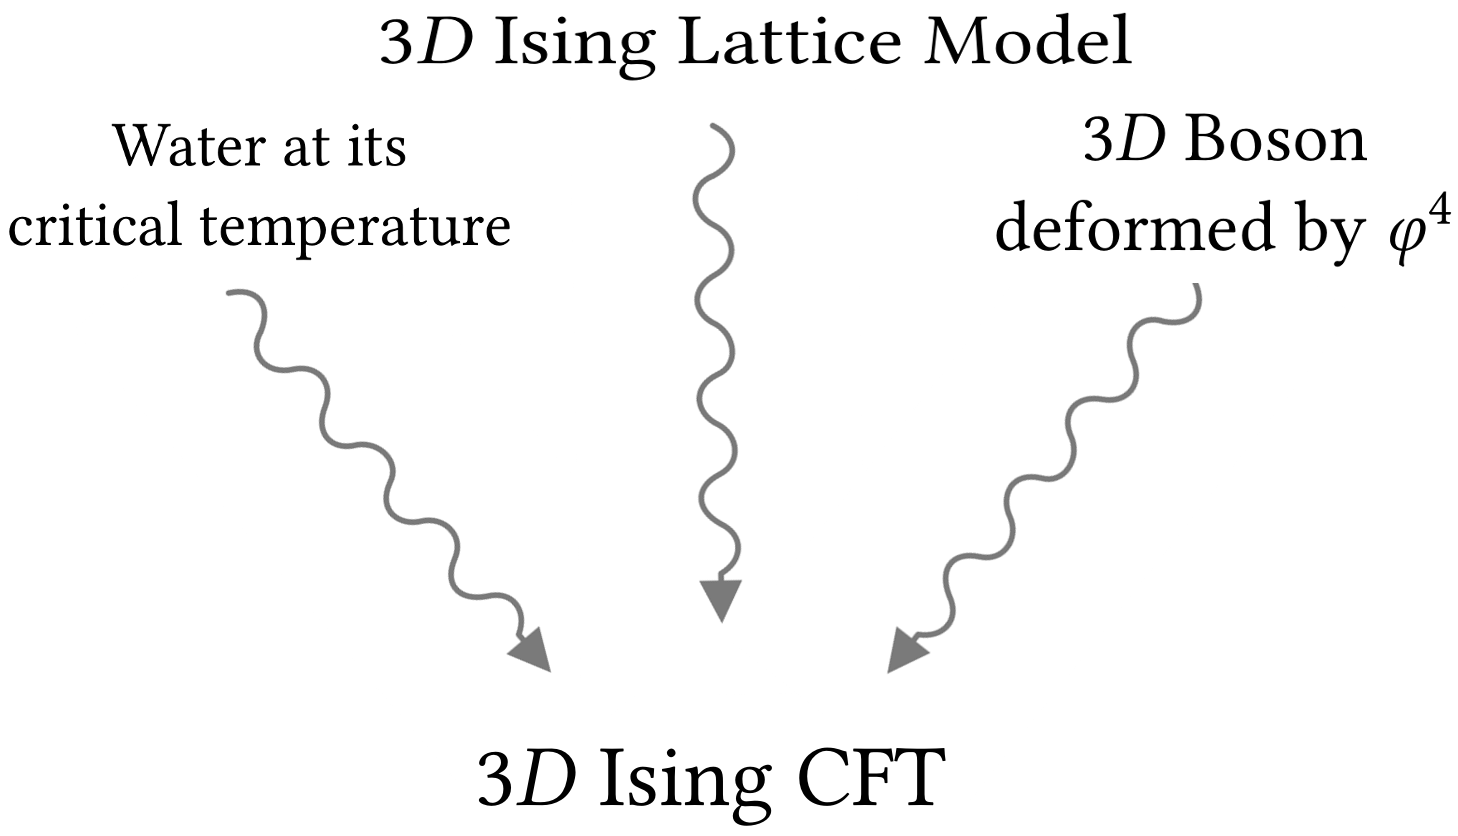
\includegraphics[scale=.16]{universality}
	\caption[IR equivalence]{\label{fig: ir equivalence}Many different phenomena at microscopic scales are described by the same conformal field theory at macroscopic scales; i.e. they fall in the same universality class! This is called \emph{IR equivalence}.}
\end{figure}

\item How do we know that we have \emph{conformal symmetry} at fixed points? Technically, all we know is that we have \emph{scale symmetry} at the fixed points and \emph{not all scale invariant theories are conformally invariant}! There are strong motivations to anticipate conformal invariance (we'll discuss these), but for now, we can take a simpler approach: we \emph{will assume} that the critical point is described by a conformal theory, compute the critical data, and check with the experiments to see if they agree!

\end{itemize}

\subsection{Using CFTs beyond statistical physics}

In the previous sections, we have used the problems in statistical mechanics to motivate the usage of \emph{conformal field theories}; indeed, as we have seen there, it is essential to understand conformal field theories to describe and compute critical data for a huge collection of phenomena.\footnote{To be fair, what is essential is to understand \emph{scale invariant theories}, which as we have already stated are not necessarily conformally invariant. Nevertheless, this is almost always the case and we'll motivate this later.} What made the study of conformal field theories all the more powerful was the concept of universality: we can divide critical phenomena into a handful of different universality classes and understanding one CFT is sufficient to understand all the problems in the same universality class. The most prominenet example of this is the $3d$ Ising universality class; solving this CFT is sufficient to understand
\begin{enumerate}
	\item Liquid-vapor transitions, e.g. water at its critical point
	\item Uniaxial magnetic systems, e.g. an idealized Nickel magnet
	\item Binary mixtures, e.g. polymer solutions 
	\item Coulombic systems, e.g. solvophobic electrolytes
	\item Micellar systems, e.g. the process of aggregation of certain surfactant molecules in dilute aqueous solutions
\end{enumerate}
Please see the section 3.1.1 of \cite{Pelissetto:2000ek} for details on these cases alongside several resources. 

Of course, there are several other universality classes and they can be used to explain yet other whole sets of phenomena in statistical mechanics, solid state physics, or chemistry; for instance
\begin{itemize}
	\item The three-dimensional XY universality class (describes the superfluid transition of $^4$He along the $\lambda-$line\footnote{See \figref{\ref{fig: lambda line}}.} among others)
	\item The three-dimensional Heisenberg universality class (describes Curie transition in isotropic ferromagnets such as Ni and EuO, among others)
\end{itemize}
where further details can be found in the latter reference, i.e. $>100$ page review \cite{Pelissetto:2000ek}.

For a practicality-minded reader, these should be more than enough as reasons to study conformal field theories. However, young researchers (especially in high energy physics) are often amazed by speculative theories or effective models in high energies, rather than low-energy phenomenological models with applications in \emph{trivial} branches, such as chemistry.\footnote{
The tone in this sentence may be uncalled for, but as a young (?) researcher in high energy physics, I'd like to make this (self-)criticism: unfortunately, we can be too focused on high energy theories and a one-theory-to-rule-them-all model that would explain whole physics and that can be best understood only in high energies. Thus, we tend to feel that things at lower energies (and branches that explain them) are secondary to what we are studying; after all, we can (?) derive them from the high energy models. This is why (for someone who thinks that way) chemistry would be labeled trivial. Of course, I'm making these comments based on my own observations, which actually form a small subset of high energy physicists, making my generalization unwarranted.

For a second, let's assume that my comment has some truth in it, i.e. some young high energy physicists do actually overemphasize the roll of high energy physics and do see some of the other branches rather trivial. Within this assumption, it is then a nonzero chance that you, the reader, may feel the same way. So I'd like to address this and hope that it is beneficial to you in case you were unaware of it.

The point is that \emph{high energy physics can be used to explain all low energy phenomena} is an assumption, and is not really back-up. It is found on \emph{constructionism}, that one can construct macroscopic behavior from the knowledge of microscopic model, but constructionism is actually not valid: there are \emph{emergent phenomena}, concepts that only emerge at long distances and cannot be explained by short distance physics. Anderson famously discusses this in his seminal paper \emph{More Is Different} in 1972, and points to the difference between \emph{reductionism} and \emph{constructionism}: we can indeed reduce low energy rules to some fundamental laws in high energy physics, but we cannot start from the fundamental laws in high energy physics and construct low energy phenomena. I strongly urge the reader to check that article if they haven't already: see \cite{Anderson:1972pca}.
} Therefore, I'd like to mention some other areas where conformal field theories are relevant.\footnote{The list is in no means complete.}
\begin{itemize}
	\item String theory, M-theory, or similar mathematically advanced models in general
	\item Flate space holography
	\item Quantum field theory
	\item AdS/CFT
	\item Cosmology
\end{itemize}

The first two items are really related to $2d$ CFTs: we know that string theory is a two dimensional conformal field theory on its worldsheet, and a scattering amplitute in four dimensional lorentzian spacetime can be related to a $2d$ Euclidean conformal field theory which lives at the null infinity of the Lorentzian space.\footnote{
This is a relatively new field and the correspondence is not really that well-established, see \cite{Pasterski:2016qvg} which roughly initiated the current research on this area. For an earnest attempt at an introductory review, see section 2 of my paper \cite{Albayrak:2020saa}.
} Our focus in these notes will be on higher dimensional $d\ge 3$ CFTs, so we can ignore these motivations.

I wrote \emph{quantum field theory} as a motivation but it is rather ambiguous so let me unpack it. As we reviewed in \secref{\ref{sec: review of RG}}, any field theory can be subjected to RG flow, and its phase diagram shows the behavior of the model in general. Even if we are not interested in critical phenomena, the fixed points are still relevant because they are like landmarks on the space of all field theories; in fact, most theories flow from a CFT at UV to another CFT at IR, see \figref{\ref{fig: UV completion}}.\footnote{This statement is probably an exaggeration. First of all, the end-points of \emph{any} QFT has to be scale invariant, but some of them are simply trivial (i.e. the correlation length $\xi=0$) and are called \emph{topological} as there is no propagating degree of freedom left in them.\footnotemark The rest have massless degrees of freedom, i.e. $\xi=\infty$, but only some of them are also conformally-invariant (there are examples of fixed points with scale invariance but not conformal invariance), and only a subset of them are interacting (hence interesting). As I do not know what are the respective ratios of these cases, I actually only made an optimistic assumption by saying \emph{most theories} in the text.} \footnotetext{
We should be very careful when we use the words trivial and topological at the same sentence! There can be many interesting non-trivial topologies, and that the theory is topological at the fixed point does not mean it doesn't have anything interesting in it. We just mean that we are not interested at those in these notes.} 
\begin{figure}
	\centering
	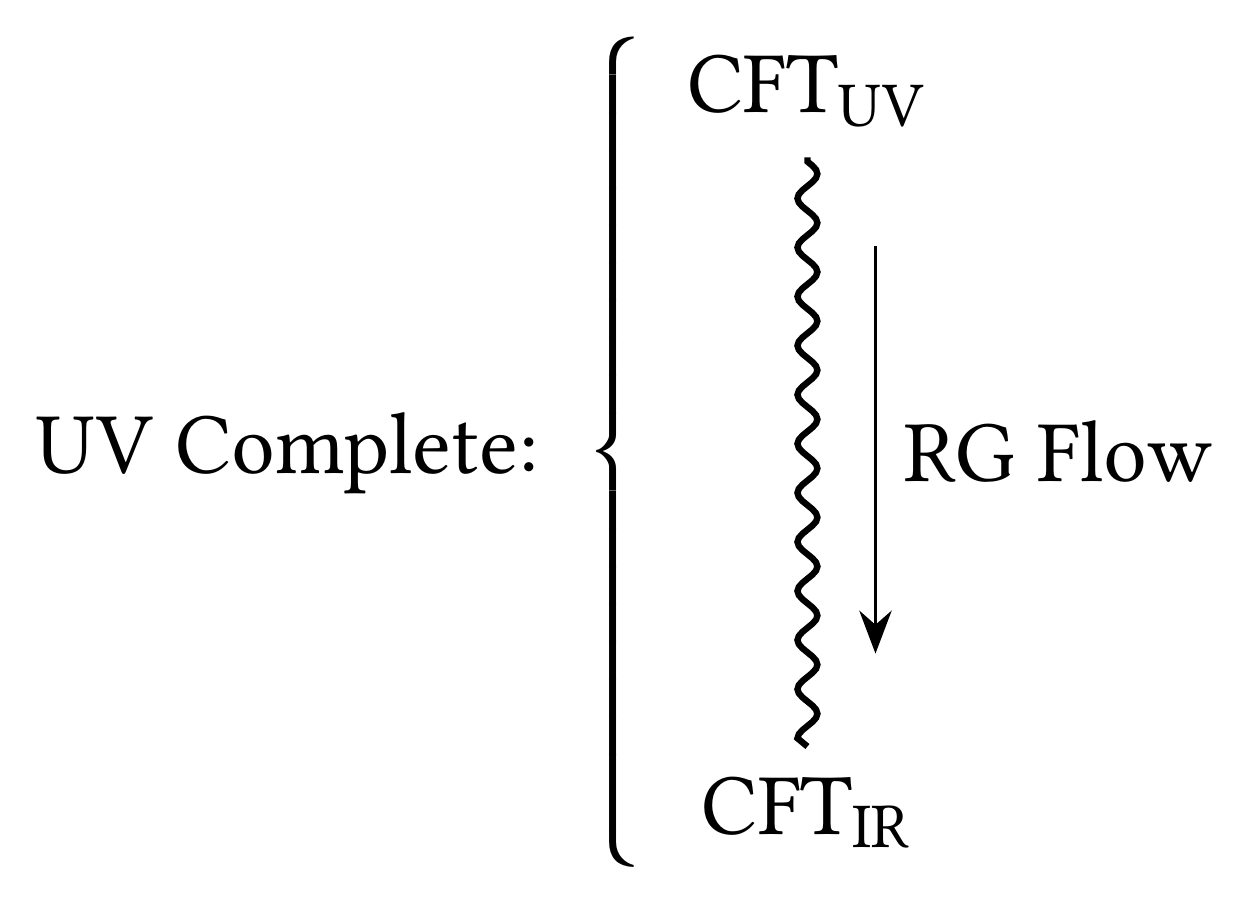
\includegraphics[scale=.35]{flow}
	\caption[End points of renormalization flow and conformal field theories]{\label{fig: UV completion}End points of renormalization flow and conformal field theories. All field theories flow from a fixed point at UV to another at IR, and fixed points are either described by a topological theory (i.e. $\xi=0$), a scale-invariant but not conformally invariant theory ($\xi=\infty$), or a conformally invariant field theory ($\xi=\infty$). Optimistically, we can assume that many cases of interest have CFTs at the end points of the RG flow.}
\end{figure}
More importantly, as we do not know how to solve strongly coupled field theories in general, we may try to expand them around CFTs;\footnote{\draftnote{I need to put some source here}} likewise, we can explain more than critical phenomena if we are close to a CFT. For instance, there is this concept called \emph{walking}, which is relevant if the theory is not scale invariant but near a fixed point,\footnote{The coupling constants are called \emph{running} as they change with scale (such as fine structure constant of Quantum Electrodynamics), and are constant if the theory is scale invariant. If the theory is almost scale invariant, the coupling constants barely change hence are called \emph{walking}!} and walking behavior is related to many things including  the electroweak phenomenology beyond the Standard Model in high energy physics and the so-called weakly first-order phase transitions in statistical mechanics.\footnote{See \cite{Gorbenko:2018ncu,Gorbenko:2018dtm} as rather introductory reviews.} Finally, a quantum theoretical model itself can be conformally invariant under various assumptions; for instance, $\SU(N)$ gauge theories with $N_f$ flavors of fundamental fermions can flow at IR to an interacting CFT for particular values of $N_f$, i.e. \emph{such gauge theories are expected to have a conformal window}, see \figref{\ref{fig: conformal_gauge}}.\footnote{For such gauge theories, Caswell \cite{Caswell:1974gg} and Banks \& Zaks \cite{Banks:1981nn} showed that there is a fixed point at the RG diagram (much like Wilson-Fisher fixed point in \figref{\ref{fig: Wilson-fisher}}, but for gauge fields instead of scalars) and that an interacting CFT lives there. This fixed point is called Caswell-Banks-Zaks fixed point, and is relevant for asymptotically free gauge theories; in particular, for the quantum field theoretical description of strong force (i.e. QCD$_4$) in its conformal window.

So what \emph{is} the conformal window? On one hand, $N_f$ is bounded from above by the requirement that the theory should have asymptotic freedom, hence $N_f\le 11N_c/2$. On the other hand, $N_f$ should be higher than some critical $N_c$ below which we get \emph{chiral breaking} which dynamically generates a length scale. The value $11/2$ above follows from perturbative computation of RG flow, and is sufficiently reliable. For $N_c$ however, we do not know any rigorous method\footnotemark, and there seems to be a disagreement to what that value should be; for instance, see Table~1 of \cite{DeGrand:2015zxa} for disagreeing results for $N_f=12$ QCD$_4$, and Table~5 of \cite{Gukov:2016tnp} for a similar situation in QED$_3$. For a conformal bootstrap approach to $4d$ CFTs at IR to which $4d$ gauge theories may flow, see \cite{Karateev:2019pvw}.

One may think that such considerations may be of theoretical importance but of little practical value; after all, we know that QCD$_4$ has three colors and six flavors, so $N=3$ and $N_f=6$; thus we do not need to consider anything else. This \naive perspective is however incorrect: as we have stressed earlier (see footnote~\ref{footnote: decoupling principle} for instance), all our theories are actually effective field theories and the effective number of flavors depend on which energy scales we are doing our experiments/computations (we can \emph{integrate-out} heavier generations). In addition, that we have found six flavors so far does not guarantee that we will not find more at higher energies, so it is advisable to fully analyze the phase diagram of $QCD$ for arbitrary values of flavor number (\draftnote{maybe I should put some references here for reasons for and against number of generations greater than 3}). Furthermore, modifications of the standard model (such as with supersymmetry) can bring further flavors, increasing the importance of considerations with higher flavor numbers (such as $N_f=12,16$, see \cite{Aoki:2011cmy}.)
} \footnotetext{To my knowledge, \emph{numerical conformal bootstrap program} is the only non-perturbative and sufficiently rigorous method for limited computational power (after all, we can always do lattice computations as well if we have large computational powers), if we are not in $2d$ and if we are not assuming other simplifications (such as supersymmetry). As we will detail later, the way conformal bootstrap tries to find $N_c$ is simple: it starts with a value of $N$, and looks for existence of conformal field theories. If $N<N_c$, we can not find any self-consistent CFT so bootstrap method should disallow all possible CFT candidates. By varying $N$, we can determine $N_c$. \draftnote{put some references here}
}To understand such concepts, we need to understand conformal field theories in higher dimensions.

\begin{figure}
	\centering 
	\begin{gather*}
		(a)\quad\begin{aligned}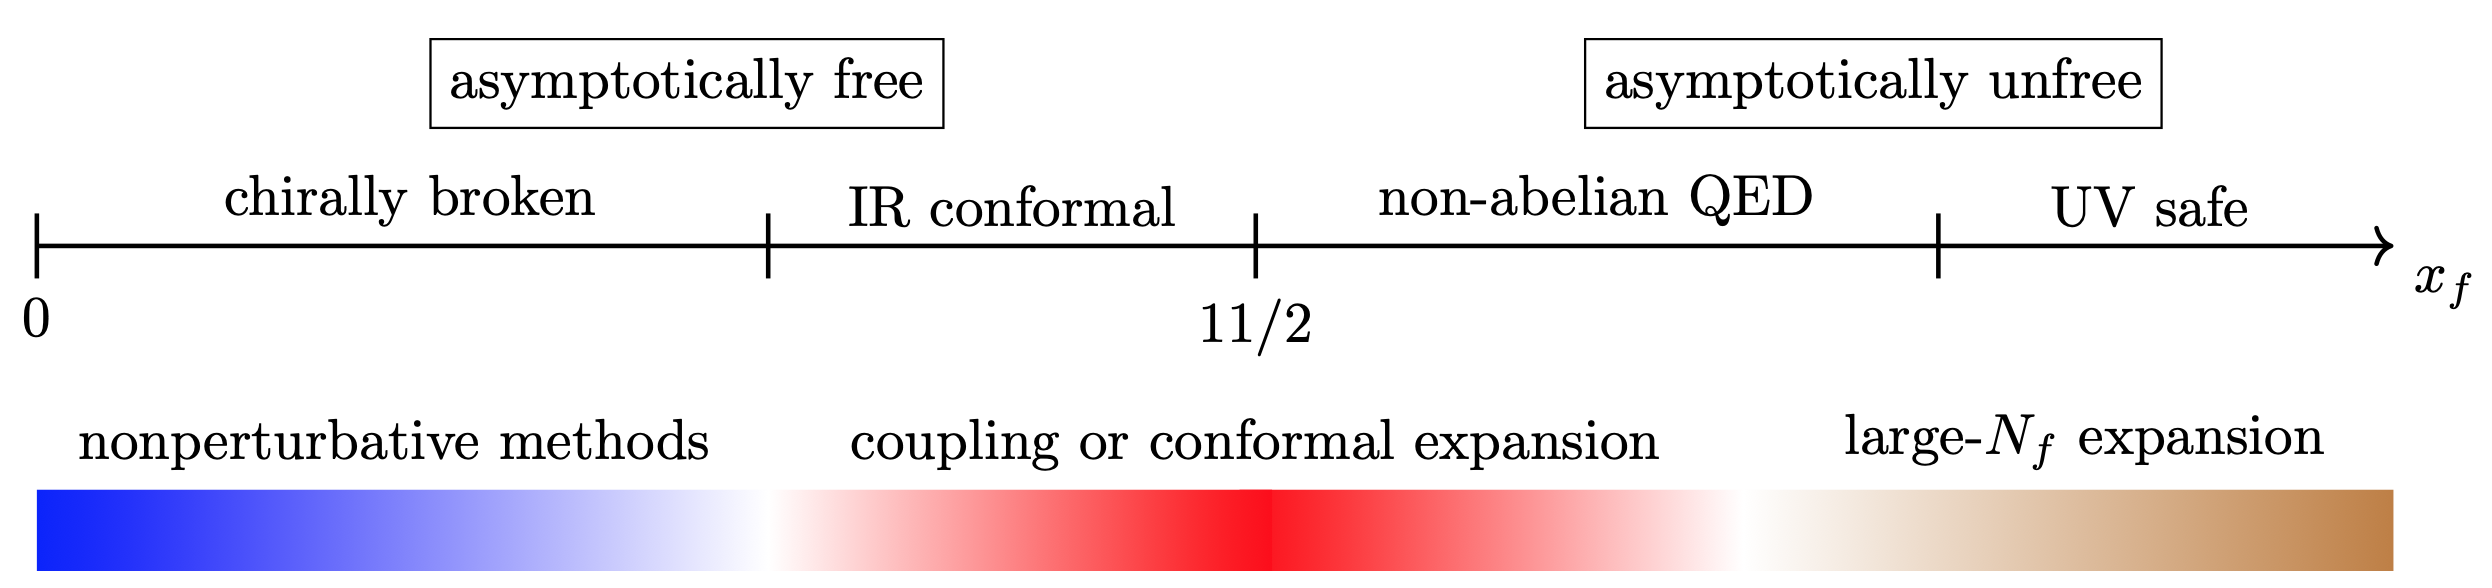
\includegraphics[scale=.315]{conformal_window.png}
		\end{aligned}\\[.2in](b)\quad\begin{aligned}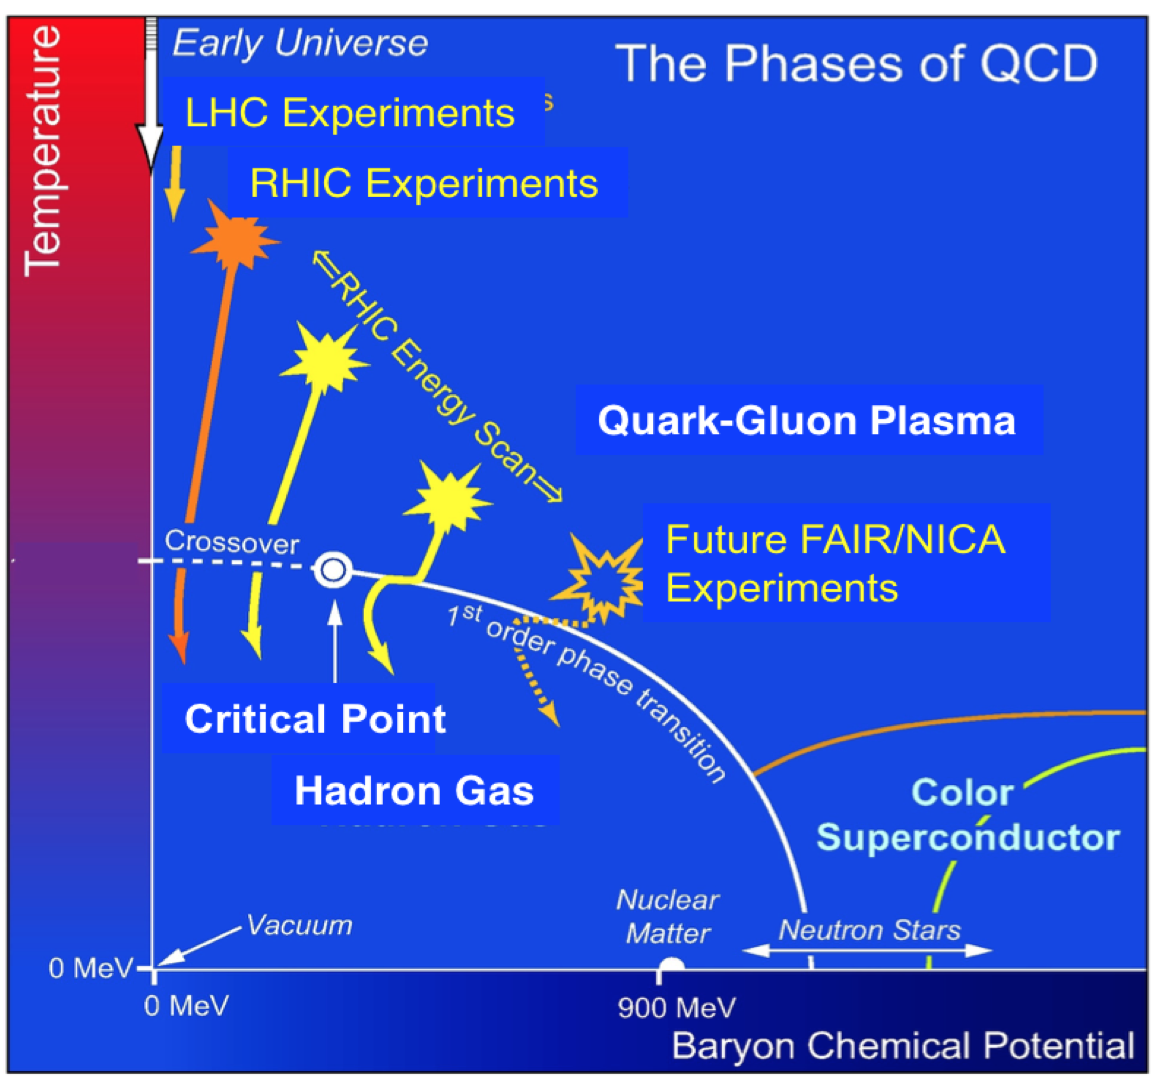
\includegraphics[scale=.6]{phase_QCD.png}\end{aligned}
	\end{gather*}
	\caption[Conformal symmetry in gauge theories]{\label{fig: conformal_gauge} \textbf{(a)} Conjectured IR phase structure for $\SU(N)$ gauge theories with $N_f$ flavors of fundamental fermions as $N,N_f\rightarrow\infty$ for fixed ration $x_f=N_f/N$, at zero temperature and zero chemical potential.  Figure taken from \cite{Lee:2020ihn}. \textbf{(b)} A schematic phase diagram for QCD$_4$ where the regions probed by different accelerator facilities are also indicated. We expect a CFT to describe the critical point and the critical manifold (the region that flows to critical point) at IR. Figure taken from \cite{Nayak:2020bjz}.}
\end{figure}

Another motivation to study conformal field theories is the infamous conjecture that there is a duality between scattering amplitudes in curved spacetime and the conformal field theory at the boundary of that space.\footnote{
More specifically, there is a correspondence between correlators in Anti de Sitter (AdS)\footnotemark in $d+1$ dimensions and the conformally invariant correlators at the boundary of that AdS \cite{Maldacena:1997re,Gubser:1998bc,Witten:1998qj}. This conjecture is often perceived as an outcome of string theory, but we can actually argue that we can arrive at this correspondence without using the string theory (at least intuitively). Penedones does a good job at pedagogically introducing this concept in \cite{Penedones:2016voo}; if you would like a more complete (yet also denser)  review, see \cite{Nastase:2007kj}.
} \footnotetext{If you have not heard of de Sitter (dS) space before, it is basically a Lorentzian version of the standard sphere in $d$ dimensions (which is Euclidean); so in a sense, it is the most symmetric space in the Lorentzian signature. AdS is almost same as dS, their only difference is the sign of the \emph{curvature} of the space. In short, flat Lorentzian space, AdS and dS are three most symmetric spaces with curvature $=0$, $<0$, and $>0$ respectively; see \tabref{\ref{table: comparison of spaces of maximal symmetry}} for a comparison of these spaces.} As we do not have the UV completion of quantum gravity,\footnote{It is often stated that \emph{we do not have a theory for quantum gravity}. This is misleading; at low energies, we know how to quantize gravity (and obtain the quanta graviton) and compute scattering amplitudes of these objects among themselves or with standard model particles. The problem is that this theory is nonnormalizable, hence predicts its own regime of validity (roughly, upto Planck scales). Thus, we \emph{have} quantum gravity but we do not know its UV completion. If we remember from footnote~\ref{footnote: normalizable vs nonnormalizable}, the situation is similar to Fermi's model of weak interactions: he had a theory for weak interactions, but it was not \emph{UV-complete}, i.e. it had to break after going higher than some energy (some energy $\sim 300$ GeV in his case).} AdS/CFT correspondence is an attractive toy model to work with the quantization of gravity in a controlled environment; indeed, AdS is simple enough to do actual computations of correlation functions of gravitons.

\begin{table}
	\centering
	\caption[Comparison of spaces with a maximal amount of symmetries]{\label{table: comparison of spaces of maximal symmetry}Comparison of spaces with a maximal amount of symmetries. The former two rows correspond to Euclidean spaces whereas the latter two do to Lorentzian spaces. It is known that not all curved spaces can be embedded in flat space; however, these spaces can actually be done so and the signature\footnotemark of the embedding space is given in the last column. See \cite{Nastase:2007kj} for a brief discussion of these points.}
	\begin{tabular}{cccc}
		\hline\hline 
		\textbf{Name of the space}&\textbf{Signature}&\textbf{Curvature}&\textbf{Signature of the embedding space}
		\\\hline
		Sphere&$(d,0)$&Positive&$(d+1,0)$\\
		Lobachevski&$(d,0)$&Negative&$(d,1)$\\
		de Sitter&$(d-1,1)$&Positive&$(d,1)$\\
		Anti de Sitter&$(d-1,1)$&Negative&$(d-1,2)$\\
		\hline\hline 
	\end{tabular}
\end{table}
\footnotetext{As an abbreviation, we write down signatures as $(p,q)$. This basically means that the metric of that space is given as $ds^2=\sum\limits_{i=1}^p dx_i^2-\sum\limits_{j=p+1}^{p+q}dx_j^2$.}

Lastly, we can mention cosmology as a motivation to study conformal field theories. By cosmological principle\footnote{The principle that states the universe is isotropic and homogeneous at sufficiently large scales. This is based on the standard model of cosmology, i.e. \emph{concordance model}, and it is calculated in \cite{Hunt:2008wp} based on this model that the inhomogeneities in the universe are below $<1\%$ for distances of $\gtrsim300$ megaparsec. The principle is widely accepted at the very least as a leading order approximation to the universe; however, this assumption is not necessarily warranted in short distances (see for instance \cite{Colin:2019opb} which claims that the principle is used incorrectly at too short distances in the analysis of supernovae data). In fact, even at large distances, there are certain examples that violate the principle, i.e. very large quasar groups that create inhomogeneities at cosmological scales (for instance \emph{Clowes–Campusano large quasar group} which is longer than $600$ megaparsec, see \hyperref{https://en.wikipedia.org/wiki/Large\_quasar\_group}{}{}{https://en.wikipedia.org/wiki/Large\_quasar\_group}). In summary, the principle is now accepted in general but may be ruled out in future, see the video \emph{New Evidence against the Standard Model of Cosmology} of Sabine Hossenfelder for a beautiful discussion of these points.
}, we expect the universe to be governed by FLRW dynamics.\footnote{FLRW stands for the initials of the scientists Friedmann, Lemaître, Robertson, and Walker. Basically, this is the most symmetric universe which expands over time, an approximate model of our own universe.} Hence, it has the metric
\be 
ds^2=-dt^2+a(t)\eta_{ij}dx^idx^j
\ee 
where $a(t)$ is called the expansion parameter. Note that $\eta_{ij}$ here stands for the spatial metric which we are taking to be flat.\footnote{In general, $\eta_{ij}$ could be the metric of a maximally symmetric $d-1$ space.} We define the conformal time $\tau$ as
\be 
d\tau=\frac{dt}{a(t)}
\ee 
hence the metric can be written as 
\be 
\label{eq: FRW metric in conformal time}
ds^2=a(\tau)^2\left(-d\tau^2+\eta_{ij}dx^idx^j\right)
\ee
We define the Hubble parameter $H(t)$ as 
\be 
H(t)=\frac{1}{a(t)}\frac{d a(t)}{dt}
\ee  

Let us now assume an inflationary cosmological model, which means that there was a time back in the early universe when there was a sustained period of accelerated expansion, i.e. \mbox{$\frac{d^2a(t)}{dt^2}>0$}. Let's assume that Hubble parameter had changed \emph{very slowly} and hence can be taken as a constant. This then implies
\be 
a(t)=e^{H(t-t_0)}
\ee 
which means $d\tau=e^{-H(t-t_0)}dt$, indicating that
\be 
\tau=-\frac{1}{Ha(\tau)}
\ee 
If we now insert this back to \equref{eq: FRW metric in conformal time}, we obtain
\be
\label{eq: dS metric}
ds^2=\frac{-d\tau^2+\eta_{ij}dx^idx^j}{H^2\tau^2}
 \ee 
But this is precisely the metric for de Sitter space in the so-called Poincar\'e frame!\footnote{\draftnote{add references here}} Thus, \emph{if universe is homogeneous, isotropic, spatially almost flat, and had expanded during an inflationary period with an almost constant Hubble constant, then the spacetime of the universe during that period is approximately given as de Sitter space!}\footnote{See \cite{Baumann:2018muz} for a detailed review of cosmology and these arguments.}

Well, how does this relate to conformal symmetries? As we review in \tabref{\ref{table: comparison of spaces of maximal symmetry}}, dS and AdS are almost same, and the boundary correlators of dS can also be explained by a CFT living there.\footnote{Unlike AdS, the CFT at the boundary of dS has to be a Euclidean CFT. One way to see this is to check the symmetries: the symmetry algebra of a conformal theory at a spacetime of signature $(p,q)$ is given as $so(p+1,q+1)$, and this should be the isometry of the space, which is roughly the last column in \tabref{\ref{table: comparison of spaces of maximal symmetry}}.} You can ask, then, why do we hear too much about AdS/CFT but not that much about dS/CFT? I'm no expert in this field but I guess we can name two sound reasons for that:
\begin{itemize}
	\item Just because the symmetries can be there does not mean they are not broken! For instance, conformal invariance is almost always broken in inflationary models\footnote{It is interesting to note that (contrary to conformal invariance) scale invariance remains an approximate symmetry in all inflationary models.} and only re-merges in slow-roll inflation\footnote{Inflation models where the \emph{potential energy} of the inflation dominates the \emph{kinetic energy}!} \cite{Baumann:2019ghk}, and even then, it is exact only in the limit where dynamic gravity decouples (so-called \emph{decoupling limit}). The interactions of slow-roll inflation beyond the decoupling limit are then controlled by the weakly broken conformal symmetry \cite{Arkani-Hamed:2015bza,Arkani-Hamed:2018kmz,Mata:2012bx}.
	
	\item Even if we had the symmetries intact, the relation between boundary CFT operators with the bulk fields\footnote{The combination ``bulk $x$'' refers to the quantity $x$ within the curved spacetime, whereas ``boundary x'' refers to the quantity $x$ at the boundary of the curved spacetime.} in AdS and dS are somewhat different. To understand this, let's rewrite \equref{eq: dS metric} again, but this time both for dS and AdS:
	\be
	ds^2=\frac{-d\tau^2+\eta^{\text{(dS)}}_{ij}dx_idx_j}{\tau^2}\quad\text{(dS)}\;,\qquad ds^2=\frac{dz^2+\eta^{\text{(AdS)}}_{ij}dx_idx_j}{z^2}\quad\text{(AdS)}
	\ee 
where $\eta^{\text{(dS)}}$ and $\eta^{\text{(AdS)}}$ are the boundary metrics respectively. We take $\eta^{\text{(dS)}}$ to be Euclidean for physical reasons (it is the metric for the spatial part of the universe), but we can take $\eta^{\text{(AdS)}}$ to be Lorentzian, meaning that a Lorentzian CFT lives at the boundary.
				
Now, we can see an intuitive difference between these two: In AdS, the CFT operators act as \emph{boundary conditions} on bulk fields; they determines bulk fields' values as $z\rightarrow 0$.\footnote{We get to the boundary as $z\rightarrow 0$.} On the other hand, the CFT operators act as \emph{final value conditions} on dS bulk fields; they determine bulk fields' value as $\tau\rightarrow 0$. We say \emph{final value condition} because, $-\infty<\tau<0$ and the CFT basically lives at the infinite future of the bulk fields. Thus it somehow makes sense to use CFT knowledge to fix the behavior of AdS fields to determine their time evaluation, but in dS, knowledge of CFT is already equivalent to the future knowledge of bulk fields, so it does not make a similar sense to use them.
\end{itemize}

Despite these reasons, CFT knowledge is essential in cosmology and the modern approach is to use it as much as possible to constraint ambiguities in the dS correlators. This approach is similar to \emph{conformal bootstrap program},\footnote{As we stated earlier, this program aims to classify and constraint conformal symmetries by non-perturbative tools such as analyticity or unitarity.} and is in fact named \emph{cosmological bootstrap program}, see \cite{Baumann:2019oyu,Baumann:2020ksv,Baumann:2020dch}.\footnote{I have been citing a lot of Daniel Baumann's papers in the last few pages. This is not just necessarily because of his papers' excellence (although they are really good): I really do not command the literature that well and am biased towards Baumann's work as I am working in his group.}

\section{What is conformal symmetry?}
\subsection{Invitation:  how Gallileon symmetry helps us derive the form for kinetic energy}
In these notes, we will analyze the effect of conformal symmetry in field theory. In the previous section, we have motivated why conformal symmetry is a relevant symmetry in many areas of physics and that it should be considered in field theories for various applications, but we did not touch on \emph{how} a symmetry can help us get any result. 

The presence of a symmetry puts many constraints on the mathematical expressions for various quantities, and we call these \emph{kinematic constraints}.\footnote{
To my knowledge, the difference between \emph{kinematic constraints} and \emph{dynamic constraints} is that the first set have to do with the motion without the source of the motion (at least in Newtonian mechanics), whereas the second set varies between different sources of motion. For instance, the relation $F=ma$ would be a kinematic equation whereas the equation $F\propto\frac{q_1q_2}{r^2}$ is a dynamic one as the former has to do with motion and is valid for any moving  object whereas the latter have to do with a particular interaction (electromagnetism) and is valid only for objects charged under this interaction. This definition generalizes beyond Newtonian physics as follows: \emph{kinematic things} (equations, constraints, data, etc.) have to do with the symmetries in the theory (hence independent of its internal details) whereas \emph{dynamic things} are model-dependent. For instance, the conservation of momentum is a kinematic constraint (i.e. it follows from the translation invariance of the theory), but conservation of parity is a dynamic constraint (it depends on which Lagrangian we choose for the model, hence model-dependent). 

I'm not aware how conventional the above nomenclature really is; furthermore, the difference between them is rather blurry in the modern perspective: take masslessness of electron for instance, it follows from gauge symmetry so one may claim it is a kinematic constraint; however, one can also argue that gauge symmetry is a property of chosen model, hence masslessness of photon is dependent on model after all. Clearly the distinction between kinematic and dynamic is not really unambiguous in such situations.

In CFT realm, the distinction between what is kinematic and what is dynamic will be somewhat more clear: anything that is fixed by conformal symmetry will be kinematic and what is left will be dynamic; for instance, three point correlators of three identical scalar operators have to have the form $\<\f(x_1)\f(x_2)\f(x_3)\>=\lambda (x_1-x_2)^{-\De}(x_2-x_3)^{-\De}(x_3-x_1)^{-\De}$. This form is a \emph{kinematic constraint} as it is fixed by the symmetry. In contrast, $\lambda$ represents \emph{dynamic data} as it is model-dependent and can't be fixed by symmetry alone.

In short, kinematic vs dynamic may/may not be a standard distinction so please take it as I have described in these notes (and blame me for any ambiguity). Even if I am be making it up, it is still consistent with the Newtonian terminology as anything that has to do with the motion (original meaning of kinematic) actually follows from the Galilean symmetry!
} In this section we will introduce and illustrate the concept of kinematic constraint with the simplest example of Galilean symmetry!

We start by the concept of kinetic energy: we observe that moving objects can exert force on other objects upon collision, i.e. move them as well, and hence they should have some kind of energy due to their motion: their \emph{kinetic} energy. We can reason that this should depend on the \emph{amount of matter} (hence the mass $m$) and on the \emph{velocity of matter} (hence $\vec{v}$), thus we say $E_k=f(m,\vec v)$ for an arbitrary function $f$.

How do we determine the function $f$? Well, we can reason kinetic energy is equal to work done on the object, and use work is the integration of force over distance, i.e. $E_k=-\De W=-\int\vec{F}\.\vec{dx}$. We can take $E_k=\De W$ as definition of work, but how about $\De W=\int\vec{F}\.\vec{dx}$? Where does this come from? Also, how do we solve this without $\vec{F}\.\vec{dx}=m\vec{v}\.\vec{dv}$ which follows from $\vec{F}=m\vec{a}$? 

Clearly using kinetic energy-work definition really cannot fix the form of kinetic energy unless we take Newton's second law and assume that the work is integration of force over distance. Well, if we are accepting $\De W=\int \vec{F}\.\vec{dx}$ to derive $E_k=m\vec{v}\.\vec{v}$, we could have accepted the latter in the first place, so this is not really a useful derivation.

Let us instead use Galilean symmetry to show that the form of kinetic energy is actually a kinematic constraint that we can derive without any other unwarranted assumptions as above.\footnote{
See \hyperref{https://physics.stackexchange.com/questions/535/why-does-kinetic-energy-increase-quadratically-not-linearly-with-speed}{}{}{https://physics.stackexchange.com/questions/535/why-does-kinetic-energy-increase-quadratically-not-linearly-with-speed} for a discussion of various derivations, including the one we'll detail below.
} Instead, we will only assume
\begin{itemize}
	\item Mass is invariant under Galilean transformations
	\item Temperature is  invariant under Galilean transformations
\end{itemize}
With these assumptions, we \emph{define} kinetic energy as the heat released once the object is brought to rest, thus it changes the temperature at a proportional rate to its kinetic energy, which we can reliably measure with a thermometer. By this definition, we can argue that the kinetic energy is \emph{additive} in mass, which we can also easily verify empirically; thus, $E_k=mf(\vec{v})$.

Let's now consider a thought experiment. We throw two identical balls of clay at each other with identical speeds, say $v$, in a train moving in the same dimension of the movement of clays with speed $v$ (see \figref{\ref{fig: Galilean}} for illustration.). For an observer in the train, the clays have initial and final kinetic energies as $(mf(\vec{v}),mf(\vec{v}))$ and $0$  respectively (note that clays merge at the collision). For an observer outside on the other hand, the initial and final energies read as $(mf(2\vec{v}),0)$ and $(2mf(\vec{v}))$. As the difference in initial and final energies have turned into heat, and as we assume the temperature is a Galilean invariant, both observers should measure same energy difference:
\begin{figure}
	\centering 
	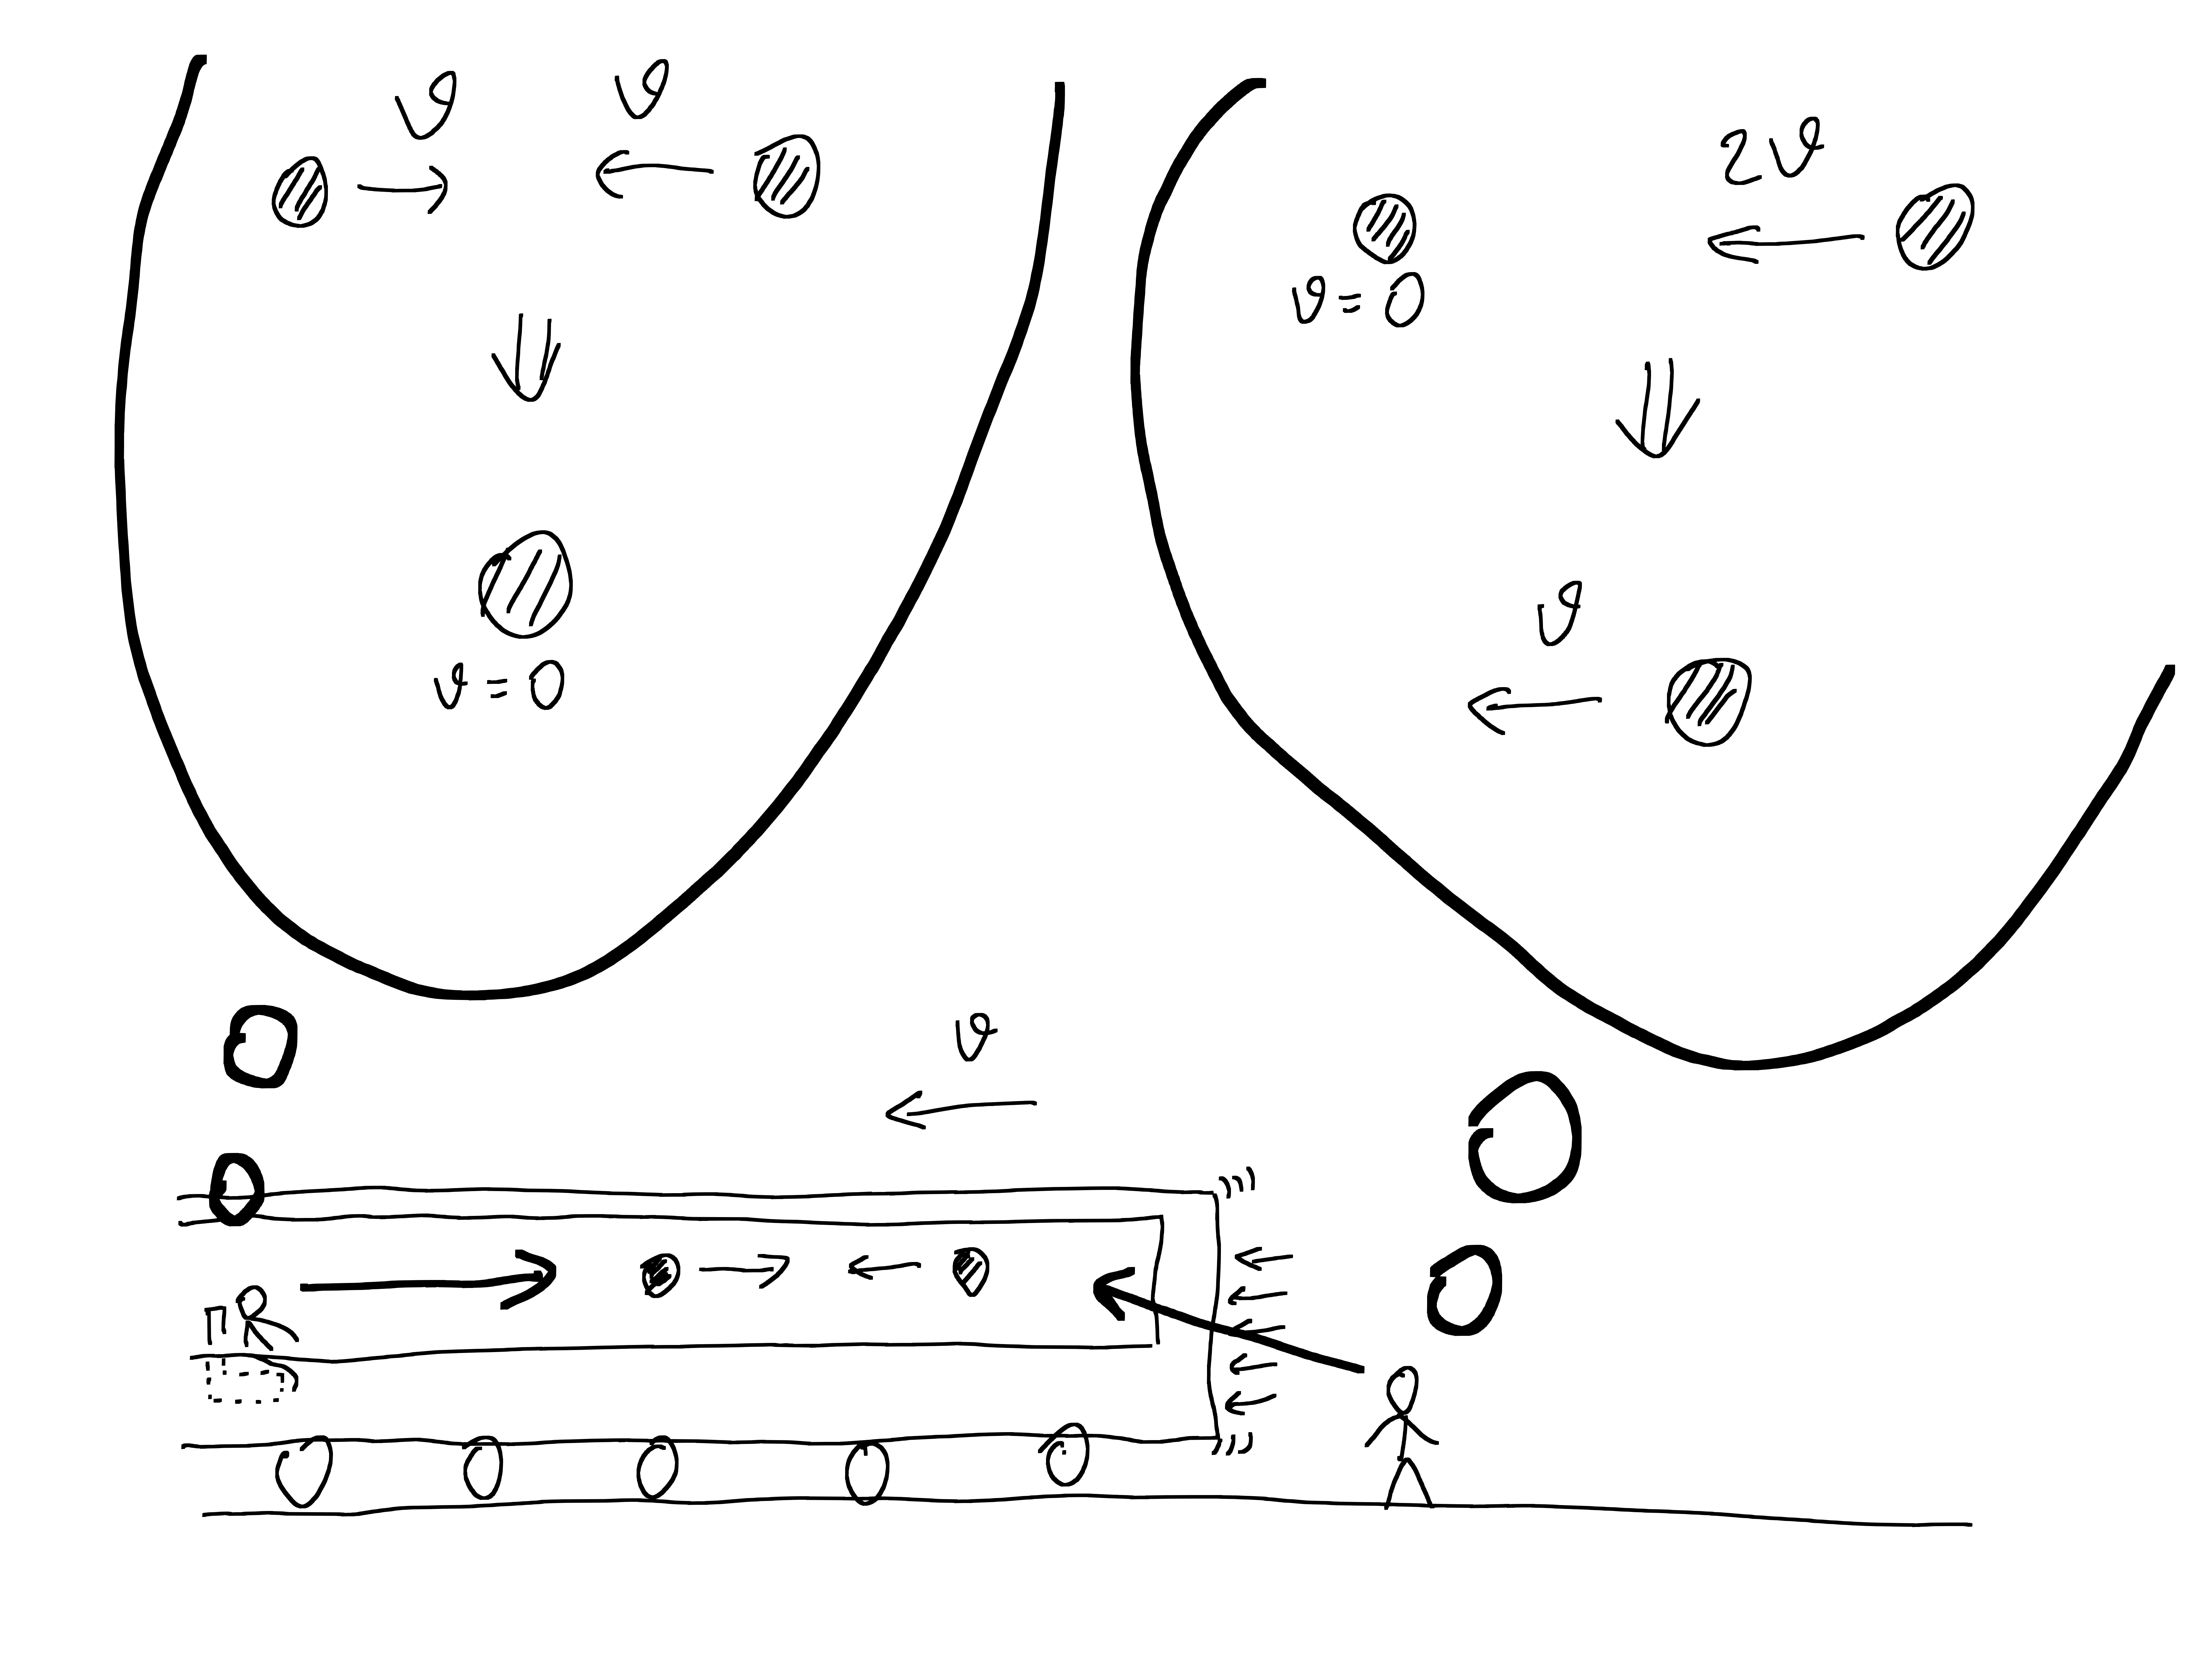
\includegraphics[scale=.05]{galilean.png}
	\caption[Constraint of Galilean symmetry on kinetic energy]{\label{fig: Galilean} Constraint of Galilean symmetry on kinetic energy. Two identical clays of mass $m$ and opposite velocities of speed $v$ collide to full stop in a train. Let $E=mf(v)$ be the formula for kinetic energy; the observer in train then observes $E_{\text{initial total}}=2mf(v)$ and $E_{\text{final total}}=0$. In contrasts, an outside observer observes  $E_{\text{initial total}}=mf(2v)$ and $E_{\text{final total}}=2mf(v)$. As the difference in energy is converted to heat (i.e. change in temperature) and as we assume that the temperature is Galilean invariant, both observers should observe same energy difference, leading to $f(2v)=4f(v)$, yielding that $f(v)\propto v^2$.}
\end{figure}
\be 
mf(\vec{v})+mf(\vec{v})-0=mf(2\vec{v})+0-2mf(\vec{v})
\ee 
which leads to $f(2\vec{v})=4f(\vec{v})$, yielding
\be 
E_k\propto m\vec{v}\.\vec{v}
\ee 
We can know consider the differential form of this equation, i.e. $dE\propto m\vec{v}\.\vec{dv}$ and use the relation $\vec{v}\.\vec{dv}=\frac{\vec{dx}}{dt}\.\left(\vec{a}dt\right)=\vec{a}\.\vec{dx}$, leading to $dE\propto m\vec{a}\.\vec{dx}$. We can then \emph{define} the force as the \emph{gradient of kinetic energy}, i.e. $\vec{F}=\vec{\nabla}E_k$, which gives us second law of Newton's law for free, i.e.
\be
\vec{F}\propto m\vec{a}
\ee 
The proportionality constants depend on our conventions and we can of course always normalize mass $m$ such that the above relation is an equality.

In this simple example, we see that assuming a symmetry brings actually a constraint to our equations: kinetic energy needs to be quadratic in velocity, which is true for any system with Galilean invariance! In the rest of the notes, we'll try to do a similar thing with conformal invariance: it will also bring various kinematic constraints which will in turn simplify the computation of numerous quantities in field theories! 

\subsection{Review: Galilean and Poincar\'e algebras}
As we have seen in the previous section, imposing invariance under a symmetry helps us constraint the physical formulae. However, to fully understand how symmetry is embedded in mathematical equations, we need to understand the concept of group and algebra, which we will briefly review here.

\subsubsection{Primer: groups, fields, and algebras}
\label{sec: review of groups, fields, and algebras}
Before we start, we may want to set the conventions and review the basics of groups, fields, and algebras. This subsection is tangential to the main direction of the notes, and can be skipped if the reader is confident in their knowledge in this area of math. In particular, this subsection can be summarized with the schematic relations shown in \figref{\ref{fig: group-field-algebra}}.
\begin{figure}
	\centering 
	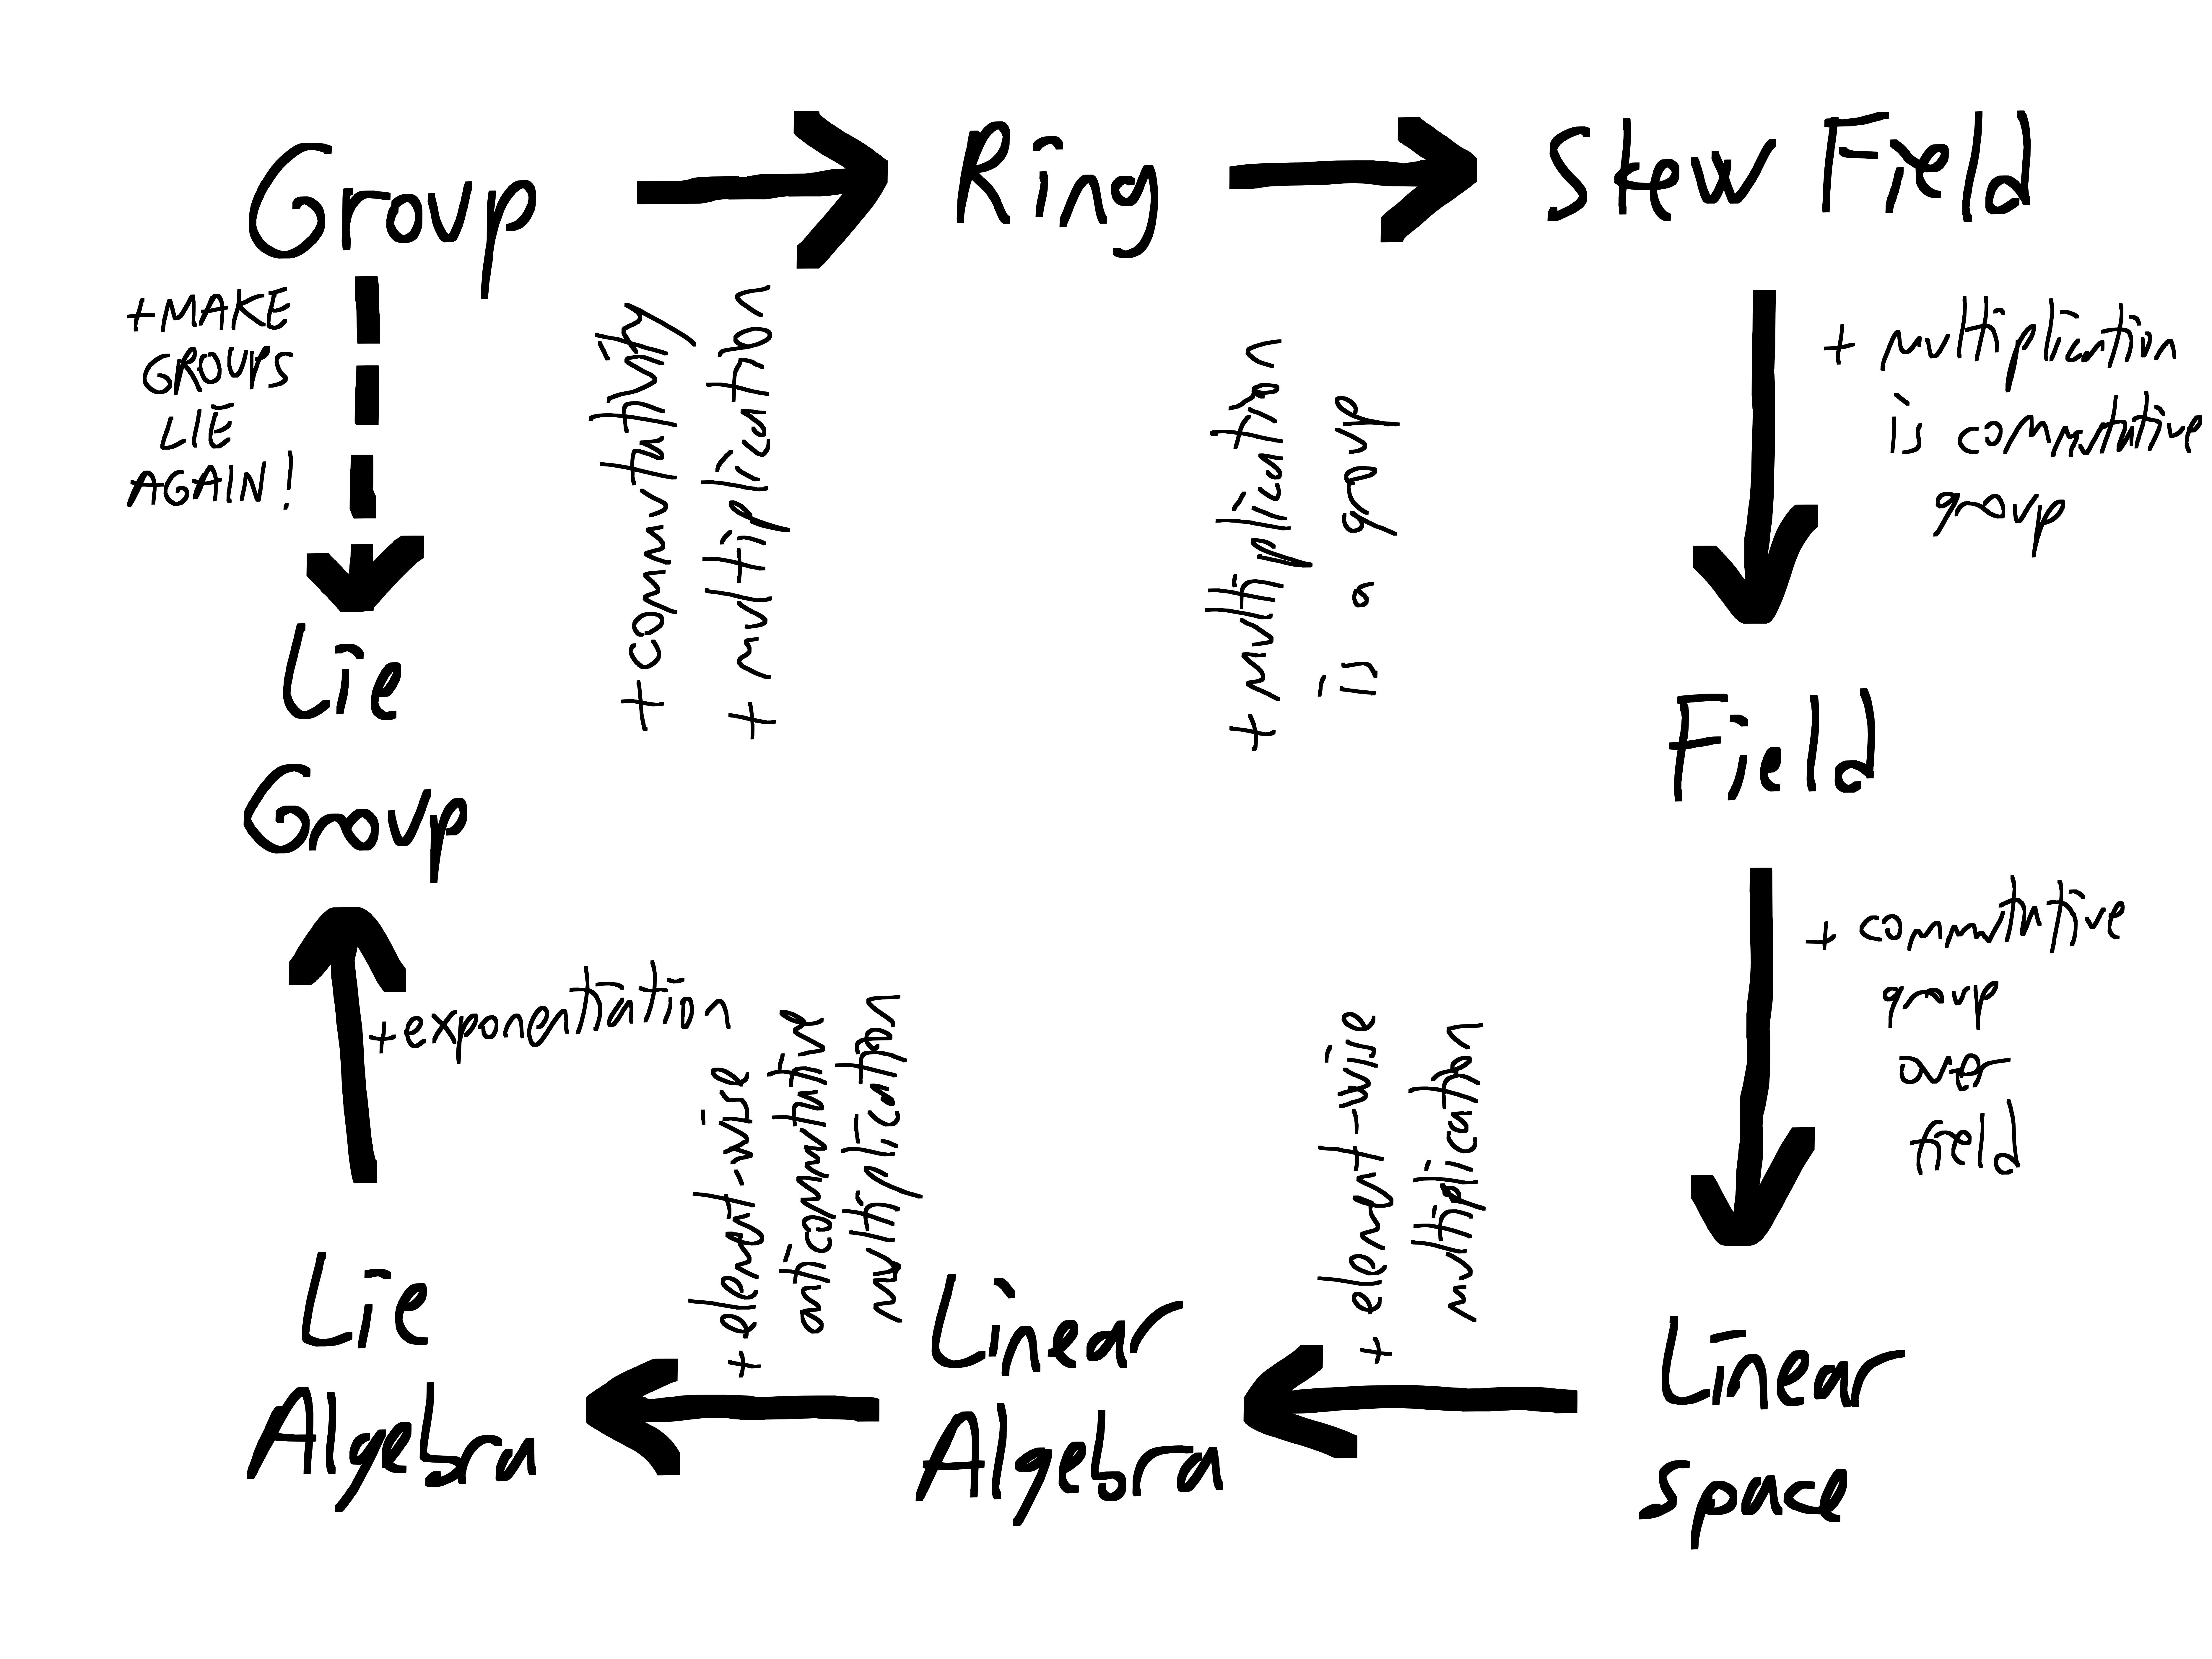
\includegraphics[scale=.05]{group-field-algebra.png}
	\caption[Schematic relation between groups, fields, and algebras]{\label{fig: group-field-algebra} Schematic relation between groups, fields, and algebras. Please see \secref{\ref{sec: review of groups, fields, and algebras}} for details.}
\end{figure}

\paragraph{Group:} A set of elements $g_i \in G$ such that
\begin{enumerate}
	\item there is a distinguished element $e$ such that $g*e=e*g=g$ for all $g$
	\item there is a mapping $g\to \hat g$ of G onto G such that $g*\hat g=\hat g*g=e$
	\item operator $*$ is associative: $g_1*(g_2*g_3)=(g_1*g_2)*g_3$
\end{enumerate}
where $e$ is usually called identity and $\hat g$ is usually called the inverse element, denoted as $g^{-1}$, and $a*b$ is denoted as $a b$. If $*$ is commutative, $a*b=b*a$ is usually denoted as $a+b=b+a$, and $\hat g$ denoted as $-g$. In this case $e$ is denoted as $0$.

$\abs{G}$ is the order of the group and is equal to the number of elements of $G$. One of the most important groups is the symmetric group  $S_n$, which is the set of all permutations of $n$ elements. In fact, in general, the collection of all transformations of a set $X$ (one to one mappings of $X$ onto itself) is a group.

Some common examples of groups include
\begin{itemize}
	\item $\C$ under addition, $\C\backslash\{0\}$ under multiplication
	\item The additive group of the ring $\Z$ (the set of integers) is called the infinite cyclic group.
	\item The additive group of the ring $\Z_n=\{0,1,\dots,n-1\}$ is the cyclic group of order $n$.
\end{itemize}

\paragraph{Ring (Commutative Group with multiplication):} Any commutative group with additional multiplication operation is called a ring; more precisely, the group $R$ is a ring if
\begin{enumerate}
	\item $R$ is commutative
	\item group operation is addition
	\item multiplication is defined in $R$ with respect to addition:
	\be 
	a(b+c)=ab+ac\;,(b+c)a=ba+ca
	\ee 
\end{enumerate}
The adjectives of the ring follows from the properties of the multiplication; for instance, if the multiplication is commutative (associative) the ring is called commutative ring (associative Ring).

The set $\Z$ (and the set $n\Z$, integers divisible by $n$) are rings under arithmetical addition and multiplication. The set $\Z_n=\{0,1,\dots,n-1\}$ is a ring under addition and multiplication module $n$. If $n$ is a prime number, it is also a field!

\paragraph{Skew field (Ring whose multiplication is a group):}  A ring $\kappa$ is a skew field if the set $\kappa\backslash \{0\}$ is a group under multiplication! They are also called division ring as division can be defined in these rings! For instance, quaternions form a noncommutative skew field. 

\paragraph{Field (commutative skew field):} A ring $\kappa$ is a field if the set $\kappa\backslash \{0\}$ is a commutative group under multiplication! For instance, $\R$ and $\C$ are fields. $\Z_n=\{0,1,\dots,n-1\}$ for $n$ prime is a also field. The main difference between a field and skew field is that multiplication is commutative in one and not in the other, i.e. $a*b\ne b*a$ for two quaternions but is so for complex numbers.

\paragraph{Linear space (A commutative group over a field):} $\cL$ is a linear space over $\kappa$ if
	\begin{itemize}
		\item  $\cL$ is a commutative group
		\item $\kappa$ is a field
		\item For all $(\lambda,x)\in (\kappa,\cL)$, there is $\lambda x\in \cL$
		\item $\lambda(x+y)=\lambda x+\lambda y$, $\lambda (\mu x)=\lambda \mu x$, $(\lambda+\mu)x=\lambda x+\mu x$
		\item $1x=x$ where $1$ is identity of $\kappa$
	\end{itemize}
Elements of linear spaces are usually called \emph{vectors}.\footnote{
We can remind ourselves following properties of vectors:
\begin{itemize}
	\item 
	Vectors $x_1,\dots,x_n$ are \emph{linearly independent} if $\sum\limits_{m=1}^{n}\lambda_mx_m=0 \Rightarrow \lambda_{1,\dots,n}=0$ for $\lambda_m\in \kappa$
\item A set $\{e_\a\}$ of vectors forms a \emph{basis} of $\cL$ if for any $x\in \cL$ we have a unique linear combination $x=\lambda_\a e_\a$.
	\item Any set of $n$ linearly independent vectors of $n-$dimensional linear space is a basis.
	\item \textbf{Dimension of $\cL$}: The maximal number of linearly independent vectors of a linear space $\cL$. If we can find arbitrary many independent vectors, $\cL$ is infinite dimensional.
\end{itemize}
} For instance $\mathfrak{M}(m,n,\ka)$ of all $m\x n$ matrices from a field $\ka$ is linear space over $\ka$, which is of dimension $m\x n$ We note that the relevant operations are element-wise addition (i.e. $M_1+M_2$) and multiplication by field elements (i.e. $cM$). For this linear space, we can always choose the basis as the matrices $e_{ij}=\delta_{ij}$.


\paragraph{Linear algebra (A commutative ring over a field $=$ A linear space with multiplication among its elements):}A linear space $\cL$ over a field $\ka$ is a linear algebra over $\ka$ if
	\begin{itemize}
		\item There is element-wise multiplication of $\cL$, hence $\cL$ is a ring
		\item $(\lambda x)y=x(\lambda y)=\lambda (xy)$ for $\lambda$ element of the field and $x,y$ element of the linear algebra
	\end{itemize}

In order to define a multiplication in a linear algebra $\cL$ of finite dimension, it is sufficient to give the product of its basis vectors:
	\be 
	e_i e_j=\sum\limits_k c^k_{ij}e_k
	\ee 
Here, $c^k_{ij}$ are called \emph{structure constants} of the algebra $\cL$.

The most common example for a linear algebra would be the space $\mathfrak(n,\ka)$ of all $n\x n$ matrices over the field $\ka$, which forms an associative and non-commutative lie algebra.\footnote{
In this algebra, the element-wise multiplication is simply the matrix multiplication, hence identity element is the identity matrix . As we can choose the basis $e_{ij}=\delta_{ij}$, the element multiplication reads $e_{ij}e_{km}=\delta_{jk}e_{im}$, which yields the structure constants $c^{rs}_{ij,km}=\delta_{ir}\delta_{jk}\delta_{ms}$.
}
	
	
\paragraph{Lie algebra (A linear algebra whose element-wise multiplication is anticommutative):}
A linear algebra $\mathcal{I}$ over a field $\ka$ is a \emph{Lie algebra} if 
	\begin{itemize}
	\item Multiplication in $\mathcal{I}$ is anticommutative.\footnote{If we have $\comm{X}{Y}=0$ for any elements $X,Y$ of a Lie algebra $\mathcal{I}$, then $\mathcal{I}$ is said to be \emph{commutative}.} They are denoted as $[X,Y]=-[Y,X]$ and are called commutator.
	\item Elements satisfy \emph{the Jacobi identity} $[X,[Y,Z]]+[Y,[Z,X]]+[Z,[X,Y]]=0$
\end{itemize}
The structure constants of a Lie algebra satisfy the identities
	\be 
	c_{ij}^k=-c_{ji}^k\;,\quad \sum\limits_{j} \left(c_{ij}^lc_{km}^j+c_{mj}^lc_{ik}^j+c_{kj}^lc_{mi}^j\right)=0
	\ee 
	Conversely, any algebra whose structure constants satisfy these conditions is a Lie algebra.
	
In general, we can obtain a \emph{Lie algebra} from any algebra $\cL$ over a field $\ka$ by choosing $[X,Y]=XY-YX$, if multiplication of $\cL$ is associative. With this construction, $\mathcal{i}$ has same elements with $\cL$.\footnote{A concrete example of this procedure is given by the set of all $n\times n$ matrices over the field $\ka$, i.e. $\mathfrak{M}(n,\ka)$, which is a Lie algebra over $\ka$. The commutation relations for its basis matrices $e_{ij}$ and the structure constants are given as
\be 
[e_{ij},e_{km}]=\delta_{jk}e_{im}-\delta_{mi}e_{kj}\;,\quad c^{rs}_{ij,km}=\delta_{ir}\delta_{jk}\delta_{ms}-\delta_{kr}\delta_{im}\delta_{js}
\ee 
} A simpler example is the set of vectors in a three-dimensional space is a Lie algebra under vector multiplication.

\begin{center}
	\bfseries\Huge 
	I have partially finished up until this point!
\end{center}

\subsubsection{Basics of exponential map: from Lie algebras to Lie groups}

\begin{itemize}
	\item what is a group?
	\item galilean transformations as a group
	\item Relativity and Lorentzian transformations
	\item Poincare group
\end{itemize}

\subsection{Scale and conformal algebras}
\begin{itemize}
	\item discussion of algebras from a pure mathematical point of view
\end{itemize}

\subsection{Conformal algebra in the framework of QFTs}
\begin{itemize}
	\item Killing equations and relevant discussion
\end{itemize}

\section{Review: Quantum Field Theory}
\subsection{some subsections}
\begin{itemize}
	\item quantum mechanics, ward identities, path integral, quantization,
	LSZ formalism, correlation functions
\end{itemize}
\subsection{Wigner's classication of operators: little group formalism}

\section{Conformal field theories}


% END
\bibliography{collectiveReferenceLibrary}{}
\bibliographystyle{utphys}
\end{document}